
\section{Object Identification and Event Selection}

In addition to the event cleaning and noise rejection requirements described in the previous section, events are selected using a cross object trigger path and are required to have at least one isolated photon with $\pt > 45 \GeV$ and $\met > 40 \GeV$. The selection is described in detail in the following sections.

\subsection{Vertex Selection}

 In the offline selection, the events are required to have at least one well identified vertex with a distance less than 24 \cm away from the nominal interaction point in $z$-direction and 2 \cm away in the $xy$-plane. The vertex corresponding to the origin of the hard-scattering process with the largest value of $\sum \pt^2$ of all associated tracks is assigned to be the primary vertex. Events required to have at least one good primary vertex (PV) where the PV must have more than 4 degrees of freedom and must be less than 24 cm away from the nominal interaction point in z and less than 2 cm away radially.

                                     
%%
\subsection{Trigger Selection}
\label{sec:trig}

The triggers used for the analysis are listed in Table~\ref{tab:triggers}. The main analysis trigger is seeded by events passing an OR of 20\GeV, 22\GeV single $e/\gamma$ Level-1 trigger. An OR of L1 seeds were originally used given that if higher then expected luminosity conditions were ever to be reached by the LHC, it was forseen that seed with the 20\GeV threshold was going to be prescaled. However the very high luminosity was never reached. 

The HLT selection requires the presence of a 30\GeV isolated photon within $|\eta|<1.4442$ and calorimetric \met $>$ 25\GeV. The trigger has further photon ID requirements such  H/E,  $\sigma_{i{\eta}i{\eta}}$, ECAL, HCAL and track isolation and $R_9$.

\begin{itemize}

\item {\bf H/E $<$ 0.10 :} Ratio of the energy deposited in the 
\item {\bf $\sigma_{i{\eta}i{\eta}} <$ 0.024 :} This variable characterizes the shape of the electromagnetic shower
\item {\bf $R_9 >$ 0.9 :} Ratio of the energy deposidted in a 3x3 square around the seed cluster to the energy of the supercluster.
\item {\bf ECAL Isolation $<$ 4.0 + 0.012 x $E_{T}$} 
\item {\bf HCAL Isolation $<$ 4.0 + 0.005 x $E_{T}$} 
\item {\bf Track Isolation $<$ 4.0 + 0.002 x $E_{T}$} 

\end{itemize} 

This trigger was implemented during the data parking program of Run2012D and recorded 7.63 \fbinv of integrated luminosity.

\begin{table}[!htbp]
\caption{ Triggers used for the main analysis and for the efficiency measurement.}
\begin{center}
\begin{tabular}{|l|}
\hline
{\bf Signal Trigger} \\ \hline
HLT\_Photon30\_R9Id90\_CaloID\_HE10\_Iso40\_EBOnly\_Met25\_HBHENoiseCleaned \\ \hline \hline
{\bf Efficiency Measurement / Monitoring Triggers} \\ \hline
HLT\_Photon30 (prescaled by 500) \\
HLT\_Photon30\_R9Id90\_CaloID\_HE10\_Iso40\_EBOnly (prescaled by 20) \\
\hline
\end{tabular}
\label{tab:triggers}
\end{center}
\end{table}

The efficiency of the Level-1 $e\gamma$ trigger has been measured by the EGM POG, and is shown in Fig.~\ref{fig:l1eff}. 


\begin{figure}[htb]
  \begin{center}
    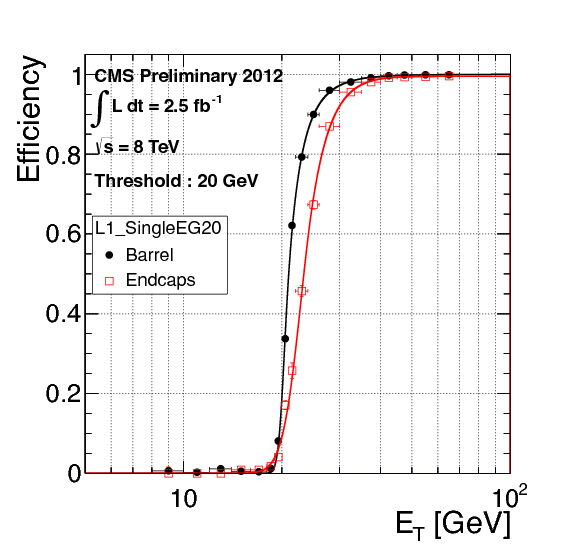
\includegraphics[width=0.48\textwidth,angle=0]{analysis_figs/EGEffVsPt.png}
    \caption{Efficiency of the 20$\GeV$ Level-1 single $e/\gamma$ trigger as a function of photon $\pt$.}
    \label{fig:l1eff}
  \end{center}
\end{figure}

Two prescaled control triggers are used to measure the HLT efficiency of the photon and $\met$ portions of main signal trigger seperately. The first control trigger is a 30$\GeV$ photon trigger with no isolation or identification selection. This trigger is used to measure the efficiency of the photon isolation and identification cuts in the main signal trigger by looking at the ratio:


\begin{equation}
  \frac{\text{passed (HLT\_Photon30 \&\& HLT\_Photon30\_Id \&\& Offline Photon Selection)}}{\text{ passed (HLT\_Photon30 \&\& Offline Photon Selection)}}.
\end{equation}

 The second control trigger is a copy of the main  signal trigger but without any $\met$ selection, and is used to meaure the efficiency online $\met$ selection by looking at the ratio:

\begin{equation}
  \frac{\text{passed (HLT\_Photon30\_Id \&\& HLT\_Photon30\_Id\_Met \&\& Offline Photon Selection)}}{\text{ passed (HLT\_Photon30\_Id \&\& Offline Photon Selection)}}.
\end{equation}

Offline selection implies that the offline reconstructed photons are  matched to the triggering online photon and passed Medium $e-\gamma$ POG ID/Isolation requirements and with an additional cut on $R_9 > 0.9$.  The results of the HLT efficiencies for the photon and $\met$ portions of the trigger are shown in Fig.~\ref{fig:hlteff} as a function of the photon \pt and particle flow $\met$, respectively. The efficiencies are fitted a to an error function and are applied to the simulated samples. The fit function used is:

\begin{equation}\label{eq:acc}
 	\frac{p_2}{2} \cdot \left( 1 + \text{Err}\left(\frac{x - p_0}{p_1 \cdot \sqrt{2}}\right)\right) %(\frac{\et - p_0}{p_1 \cdot \sqrt{2} })
\end{equation}

and the parameters are given in Table \ref{table:trigfits}.

\begin{table}[!h]
\centering
 \caption{The fit parameters for the trigger efficiency curves}
 \label{table:trigfits}         
 \begin{tabular}{|c|c|c|}
   \hline
   Parameter     &  Id Efficiency & Met Efficiency\\ 
   \hline
   \hline
  $p_0$ & 19.4 $\pm$ 7.1  &  28.2   $\pm$ 0.1 \\
  $p_1$ & 7.1 $\pm$ 4.5   &  25   $\pm$ 0.3 \\
  $p_2$ & 0.89$\pm$ 0.005 & 0.98 $\pm$ 0.003 \\
\hline          
 \end{tabular}
\end{table}

We have used a variable bin size in the efficeincy plots, to demonstrate that the fitted values represent the behviour in all energy ranges. We have further shifted the central values of the fits within their errors to estimate the unceratinty, and found it to be less than $0.05 \%$.

\begin{figure}[htb]
  \begin{center}
    \begin{tabular}{cc}
    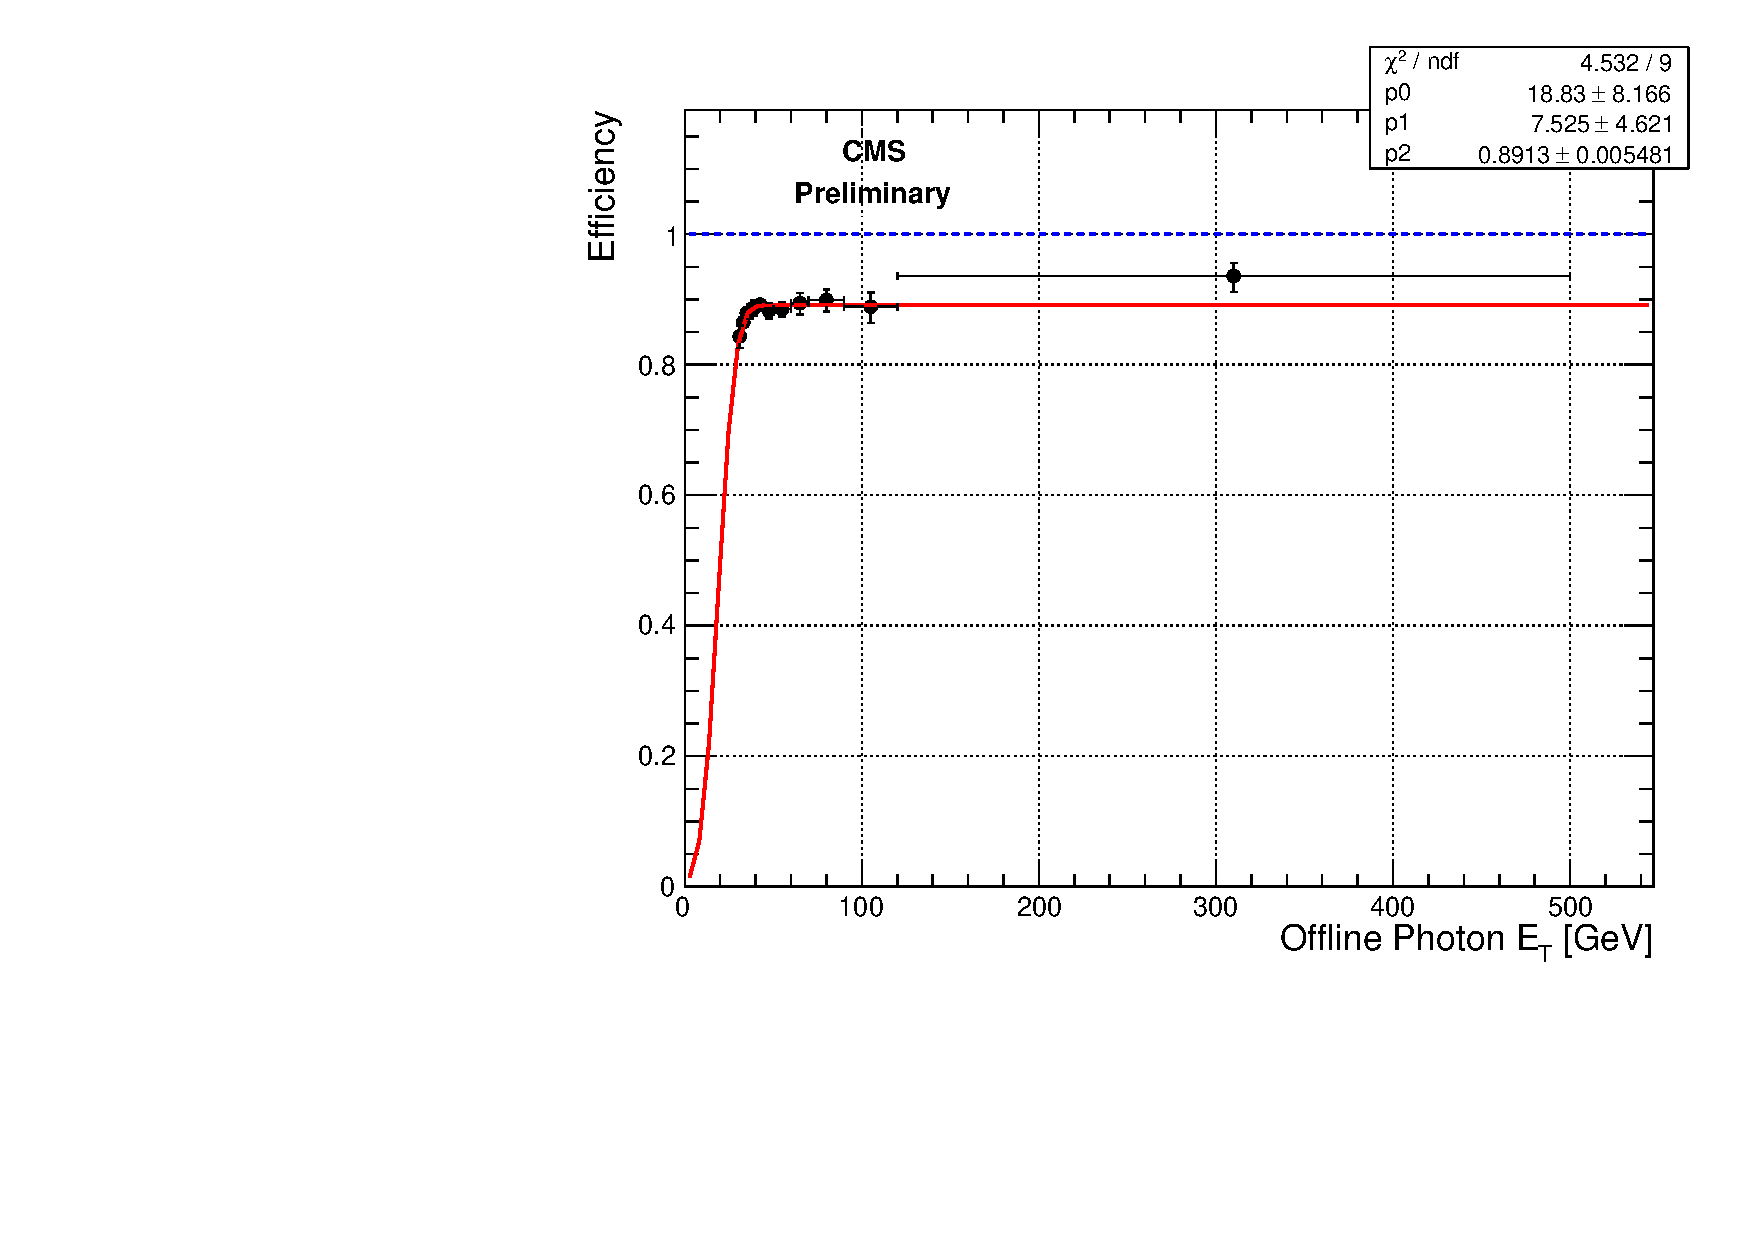
\includegraphics[width=0.48\textwidth]{analysis_figs/eff_id_vspt.pdf}
    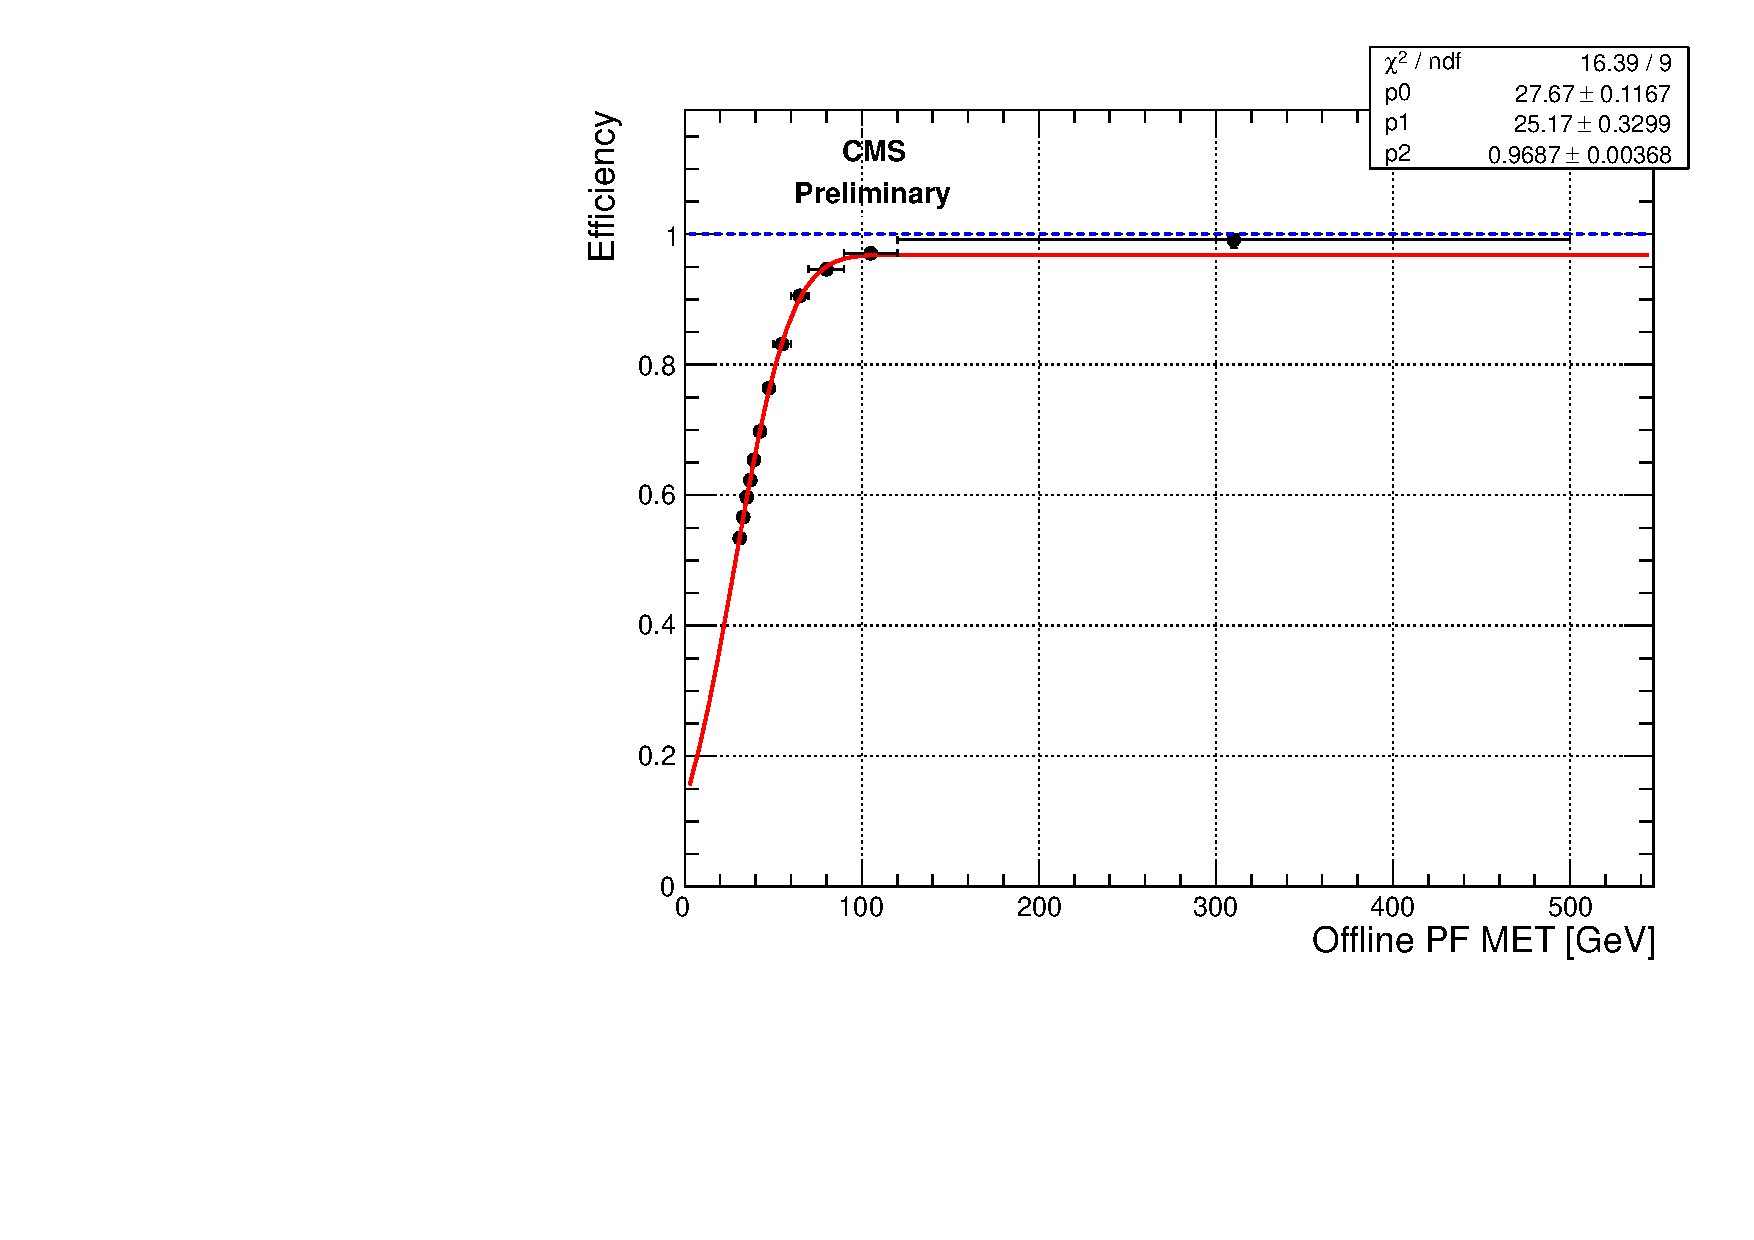
\includegraphics[width=0.48\textwidth]{analysis_figs/eff_met.pdf}
    \end{tabular}
    \caption{Efficiency of the HLT photon selection as a function of offline reconstructed photon \pt (left) and efficiency of the HLT $\met$ selection as a function of offline reconstructed particle flow $\met$ .}
    \label{fig:hlteff}
  \end{center}
\end{figure}

%%
\subsection{Photon Reconstruction \& Selection}
\label{sec:photonid}
The photon candidates are reconstructed from clusters of energy deposited in the ECAL and merged into superclusters. The photon object is required to have $\pt > 45 \GeV$ and be within the barrel fiducial region of the detector ($|\eta | < 1.4442$). The photon is also required to be isolated using the identification variables recommended by the EGM POG \cite{PhotonID}. With a signal efficiency greater than 80\% in this range, the EGM Medium photon ID includes the following selection:

\begin{itemize}

\item {\bf Particle Flow Photon Isolation :} Sum of $\pt$ of all photons within a cone of $\Delta R = 0.3$, excluding a strip in $\eta$ of 0.015 around the supercluster, is required to be less than $0.7+0.005 \times \pt^{\gamma}$
\item {\bf Particle Flow Charged Isolation :} Sum of $\pt$ of all charged hadrons within a hollow cone of $0.02 < \Delta R < 0.3$ around the supercluster, is required to be less than $1.5$ GeV.
\item {\bf Particle Flow Neutral Isolation :} Sum of $\pt$ of all neutral hadrons within a cone of $\Delta R = 0.3$ around the supercluster, is required to be less than $1.0+0.04 \times \pt^{\gamma}$.
\item {\bf Single tower H/E :} Ratio of the energy deposited in the single closest HCAL tower to the supercluster position and the energy deposited in ECAL to that supercluster is required to be less than 0.05
\item {\bf $\sigma_{i{\eta}i{\eta}}$:} The width of the shower in i{$\eta$}-space is required be less then $0.011$ . The lateral extension of the shower, $\sigma_{i\eta i\eta}$, is measured in terms of the energy-weighted spread within the 5 X5 crystal matrix centred on the crystal with the largest energy deposit in the supercluster. The symbol ieta (or if, ix, or iy used in the following) indicates that the variable is obtained by measuring position by counting crystals.
\item {\bf Pixel Track-Seed veto:} Consisting of at least two hits in the pixel detectors suggest a charged particle trajectory which would arrive at the ECAL within some window defined about the photon supercluster position. To minimize the contribution from misidentified electrons, events with such hits are rejected.
\end{itemize}

In addition to the medium id/isolation photon selection, we require a $R_9$ cut.

{\bf R9 Selection:} R9 variable measures the overall transverse spread of the shower. It is the ratio of the energy deposited in ECAL inside a 3$\times$3 crystal matrix centered on the most energetic crystal in the supercluster and the superCluster raw energy. To fully cover the trigger requirements, $R_9 > 0.9$ is required. 

The photon isolation cone is susceptible to pileup from interactions not corresponding to the primary vertex. The correction from the pile-up energy contribution to the photon identification is applied using the following equation:
\begin{equation}
Iso^{new}  = Iso^{Original} + (\rho * A_{eff})
\end{equation}
where energy density $\rho$, is the median background density per unit area and a measure of the pile up activity in the event. $A_{eff}$ , the effective area is defined as the ratio of the slope obtained from linearly fitting Iso(Nvtx) to the one from linearly fitting $\rho$(Nvtx). 

The standard tag-and-probe tool is utilized to measure the efficiency of the photon ID in data with $Z\to e^{+}e^{-}$ events. Tag-and-probe is a method of using the redundant identification of electrons (e.g. both tracker and ECAL information) to estimate the efficiency of the photon selection in data. The photon selection has been designed to have similar efficiency for electrons and photons.  Thus any relevant data effects should be visible in clean samples of Z boson decays and allow for a correction to the photon MC. The actual product of these studies is a Data/MC ratio which can be applied to correct the MC efficiency.

The correction factor corresponding to our identification (photons with R9$>0.9$) efficiency is given in Table\ref{photon_table} as provided by the EGM group. This correction is applied to our MC and included in the final systematic uncertainty on the efficiency.

\begin{table}[!h]
\small
\centering
 \caption{Scale Factors for the EG Photon Id}
 \label{photon_table}
 \begin{tabular}{|c|c|c|c|}
   \hline
   Variable     &  [30 - 40 \GeV] & [40 - 50 \GeV] &  [50 - \GeV] \\
   \hline
   \hline
Pixel Seed Veto & 0.9954 $\pm$ 0.0047 $\pm$ 0.0002 & 0.9707 $\pm$ 0.0165 $\pm$ 0.0017 & 1.0122 $\pm$ 0.0142 $\pm$ 0.0024\\  
EG Id ($<0 < |\eta| < 0.8$) & 0.9962 $\pm$ 0.0100 & 0.9966 $\pm$ 0.0100 & 0.9960 $\pm$ 0.0100 \\
EG Id ($<0.8 < |\eta| < 1.5$)& 0.9967 $\pm$ 0.0100 & 0.9970 $\pm$ 0.0100 & 0.9971 $\pm$ 0.0100 \\
\hline
 \end{tabular}
\end{table}


\subsection{Anomalous Signal Rejection}
\label{sec:BH}
In addition, to reduce the non-collision background from halo and anomalous calorimeter signals, photons are required to pass the selection described below :

\begin{itemize}
\item {\bf $\sigma_{i{\eta}i{\eta}}$: } $> 0.001$ for spike removal
\item {\bf $\sigma_{i{\phi}i{\phi}}$: } $> 0.001$ for spike removal
%\item Absolute value of the largest intra-cluster time difference ({\bf LICTD}) between crystals with more than 1 \GeV deposited  $<$ 5 ns. This cut ensures that the energy deposition is consistent both in the pattern of the energy deposition and in the timing with respect to prompt photon candidates from collision.
\item {\bf angle} $>1.2$ where the angle is derived from the RecHits and are used to define the angle that the major axis makes to the phi direction. This variable tells us how well the cluster is aligned with the z-axis. If the angle is small (closer to 0) then the shower is elongated parallel to the beam. If the angle is closer to $\pi/2$ then the shower is elongated perpendicular to the beam.
\item {\bf $R_9$ } $< 1$ for spike removal
\item {\bf Swiss-cross-like requirement:} Ratio of seed crystal energy to energy in the energy in a  cross 3 crystals in $i{\eta}$ and 5 in $i{\phi}$ is less than 0.9. %Detailed description of this cut can be found in Appendix \ref{App:AppendixA}.
%\item {\bf Seed crystal time} within 3 ns of prompt for halo removal
\end{itemize}

%We calculate the efficiency of the LICTD by selecting $Z \to \mu \mu \gamma$ events in both data and MC by requiring a good photon  with \pt  $> 15 \GeV$ and the selection cuts above except LICTD cut, and 2 good global isolated muons with \pt $> 20\GeV$. Muons are further required to be separated from each other by $\Delta R > 1.0$. In addition, the two body mass of the dimuon system is required to be $ < 80\GeV$ and the three body mass of the $\mu\mu\gamma$ system is required to be within 80 - 100 \GeV to ensure radiative decays. The efficiency for the LICTD cut is measured to be {\bf XXXXX }. 

\subsection{Electron and Muon Rejection}

\label{sec:lepton}

In this analysis, we minimize the existence of any loosely defined electron or muon to minimize contributions from the standard model backgrounds such as W$\gamma$.  Electron candidates are reconstructed from a collection of electromagnetic clusters compatible with  a track. The momentum of the electron track is fitted using a Gaussian Sum Filter (GSF) algorithm along its trajectory with the algorithm taking into account the possible emission of Bremsstrahlung photons in the silicon tracker. 

The {\bf electron selection} criteria for the veto are as follows:

\begin{itemize}
\item $\pt>10\,\GeV$
\item $\Delta R$ between the photon in the event $>0.3$
\item $|\eta| < 2.5$; excluding the barrel and endcap transition region ($ 1.4442 < |\eta_{sc}| < 1.566$)
\item Cut-based electron ID ``Veto'' requirement
\item Particle Flow based relative isolation  is required to be less than $ 0.15$. The recommended $\rho$ pileup corrections are applied
%\item Transverse impact parameter of the electron with respect to the beamspot $ < 0.02$~cm.
\end{itemize}

The {\bf muon selection} relies on the ``Loose'' definition of muons from the baseline muon selection provided by the muon POG~\cite{muonid}. The selection criteria are: 

\begin{itemize}
\item  $\pt > 10$\,\GeV
\item  $|\eta| < 2.1$
\item Classified as GlobalMuon or Tracker Muon with Particle-Flow muon ID
\item Particle Flow based relative isolation  is required to be less than $ 0.2$. The recommended $\Delta \beta$ pileup corrections are applied~\cite{TQRS}
\item $\Delta R$ between the photon in the event $>0.3$.
\end{itemize}

%%
\subsection{Jet Reconstruction \& Selection}
\label{sec:jet}

PF Jets are reconstructed using the anti-k$_T$ algorithm~\cite{Cacciari:2008gp} with a distance parameter of 0.5 (AK5). Pileup jet ID is applied, where the identification relies on: the trajectories of tracks associated to the jets  inside the tracker acceptance, and the topology of the jet shape and the object mujltiplicity. For the simulated samples, the jet $\pt$ is smeared ($\sim$ 5-29\% depending on $\eta$) to account for the better jet energy resolution seen in the MC compared to data~\cite{JetResolutiontwiki}. Jets that are identified as non-pileup and have a \pt $ > 30 $\GeV are used in various cut levels in the analysis. Depending on the cut level, we require the following jet related selection requirements.

{\bf HT}: is defined as the scalar sum of the jet transverse momenta (of the selected jets based on the identification criteria outlined above). We reject events with large hadronic activity by requiring HT $<100 \GeV$.

{\bf Number of Jets}: we require the number of identified jets in the event to be less than 2.

{\bf $\Delta\Phi$(Jet,Photon)}: we require photons and identified leading jet not to be back to back by imposing  $\Delta\Phi < 2.5$ 


%\clearpage
%%
\subsection{MET Reconstruction \& Selection}
\label{sec:met}

The \met in the event is calculated using the particle flow algorithm with Type-I and Type-0 corrections. These corrections account for the jet energy corrections and also compansate for the degradation of the \met reconstruction due to the pile-up interactions. Furthermore, the smearing of jets are propagated into \met. 

Lastly the $xy$-shift correction is derived and applied to reduce the $\phi$ modulation in \met for MC and data seperately. To correct for the modulation, a linear function is fitted to the correlation between the average of the $x$ and $y$ ($<\Em_x>$ , $<\Em_y>$) components of the \met and the number of vertices in the event ($N_\mathrm{Vtx}$). %The 2D distributions are shown in Fig. \ref{fig:xy_shift} both for data and MC. 


%\begin{figure}[htbp]
%  \begin{center}
%    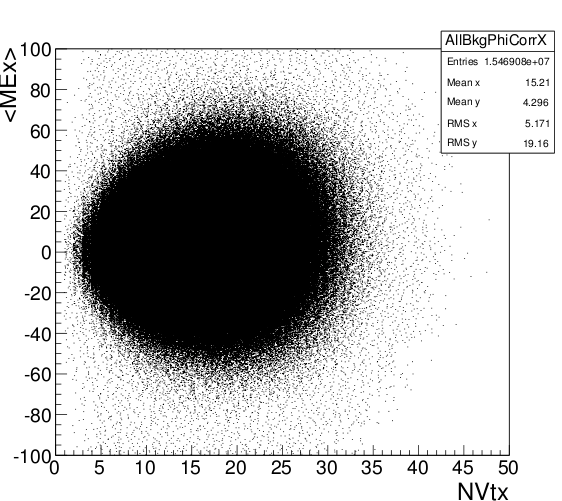
\includegraphics[width=0.45\textwidth]{analysis_figs/2D_x.png}
%    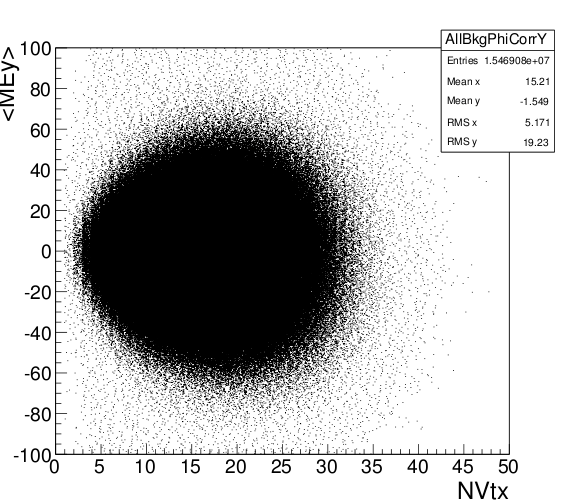
\includegraphics[width=0.45\textwidth]{analysis_figs/2D_y.png}
%    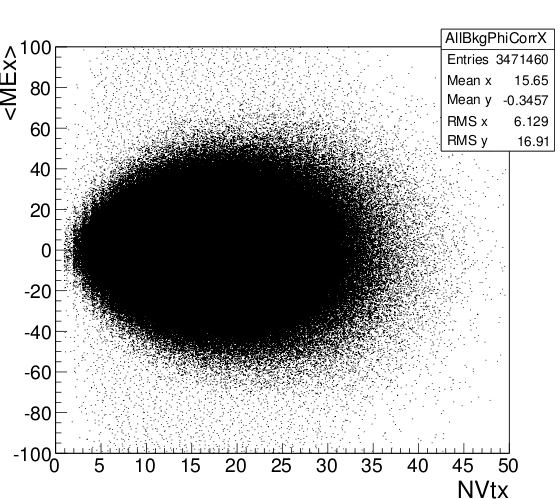
\includegraphics[width=0.45\textwidth]{analysis_figs/2D_x_mc.png}
%    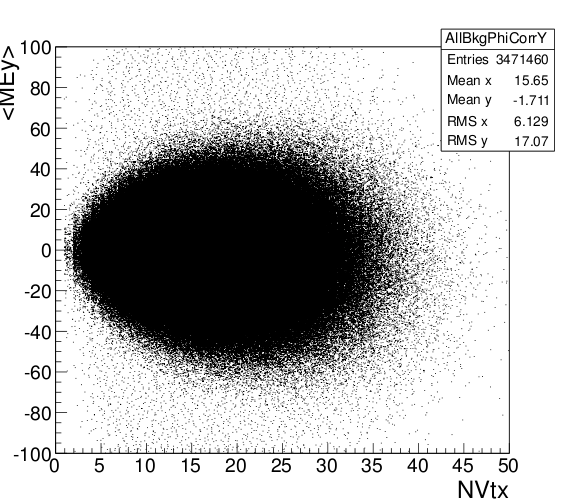
\includegraphics[width=0.45\textwidth]{analysis_figs/2D_y_mc.png}
%    \caption{ 2D plots related to the MET $\phi$ modulation for (top row) data, (bottom row) mc }
%    \label{fig:xy_shift}
%  \end{center}
%\end{figure}

In the 2D disctributions, all MC the backgrounds are included with appropriate normalizations and a generalized fit is extracted. The correction factor from the fit is then applied on all MC. Data on the other hand, also includes all the data-driven backgrounds. The fit extracted is applied on data and the data-driven backgrounds to correct for the modulation. These fits can be seen in Fig. \ref{fig:metfits}

\begin{figure}[htbp]
  \begin{center}
    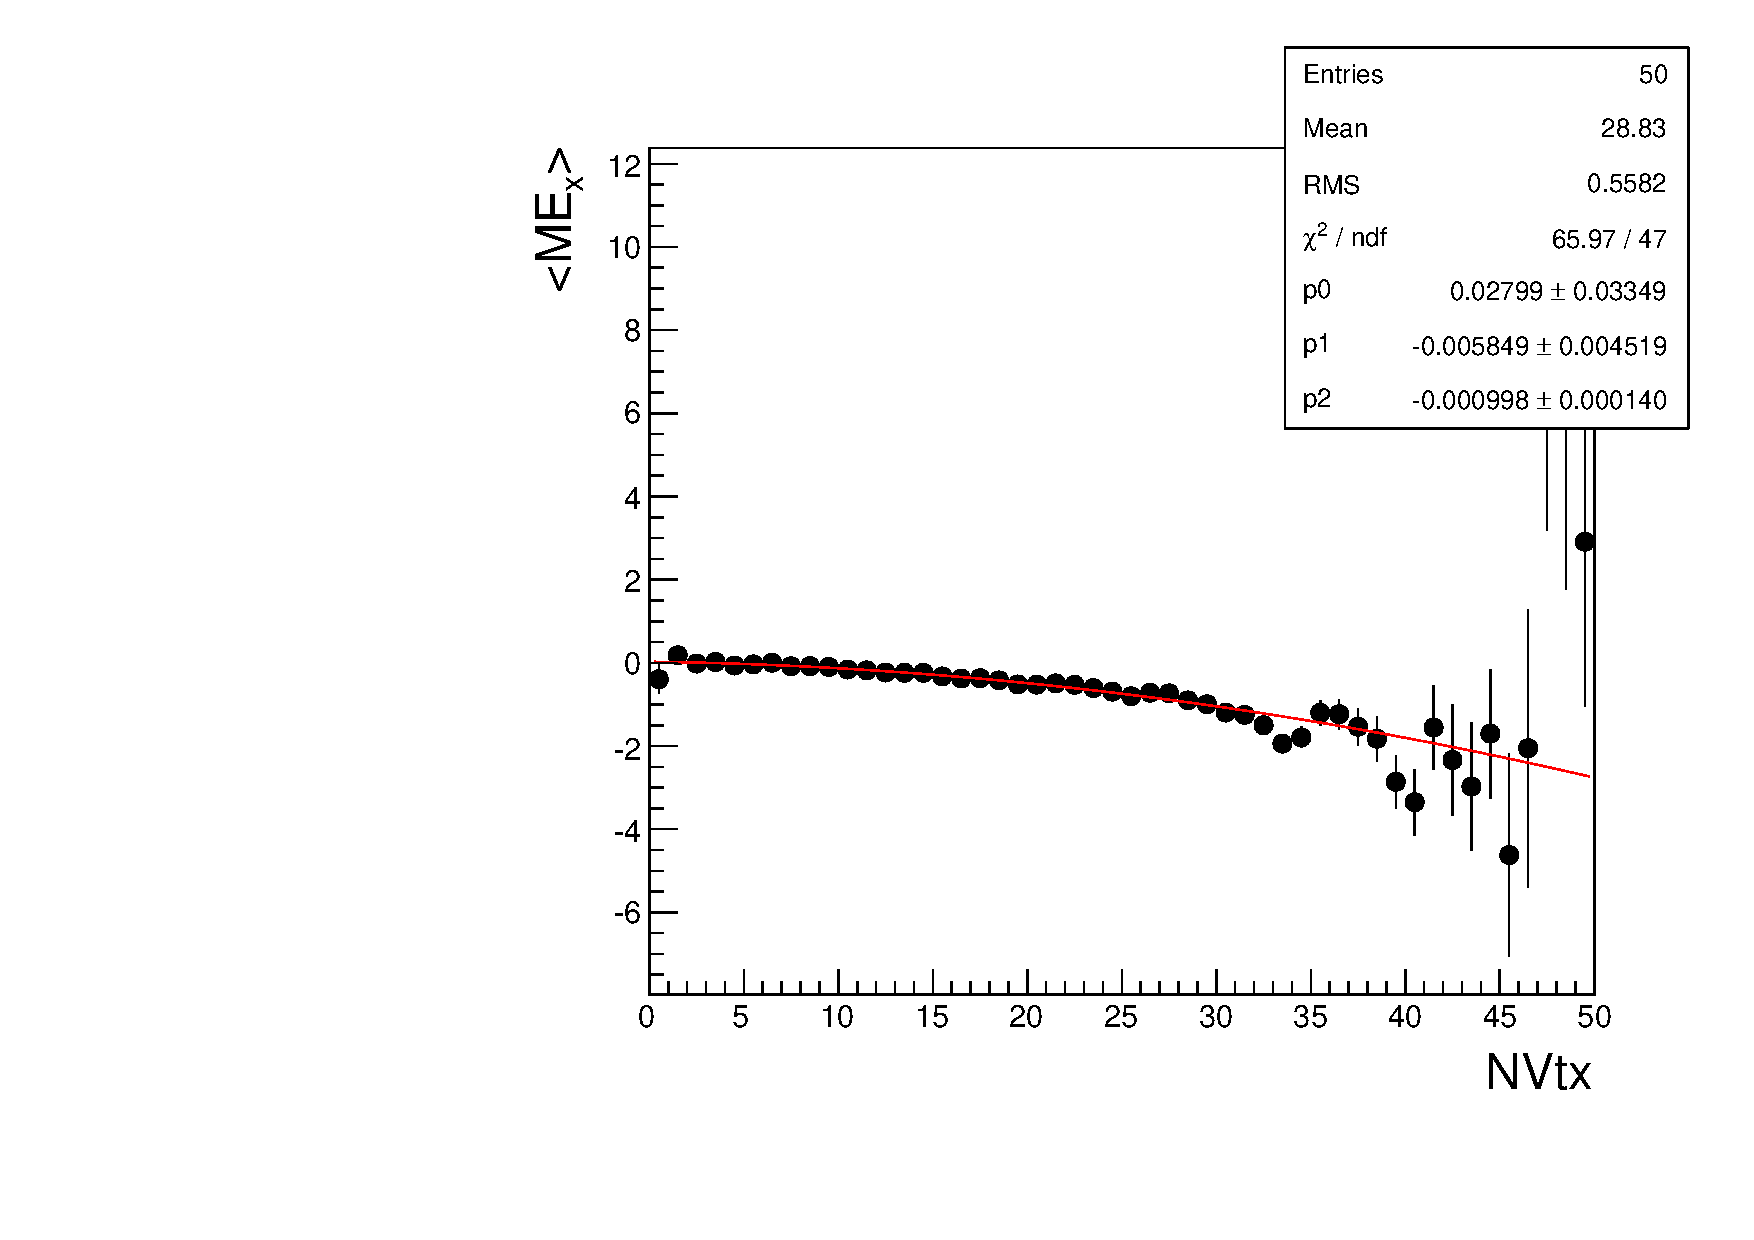
\includegraphics[width=0.45\textwidth]{analysis_figs/linear_fit_mcx.pdf}
    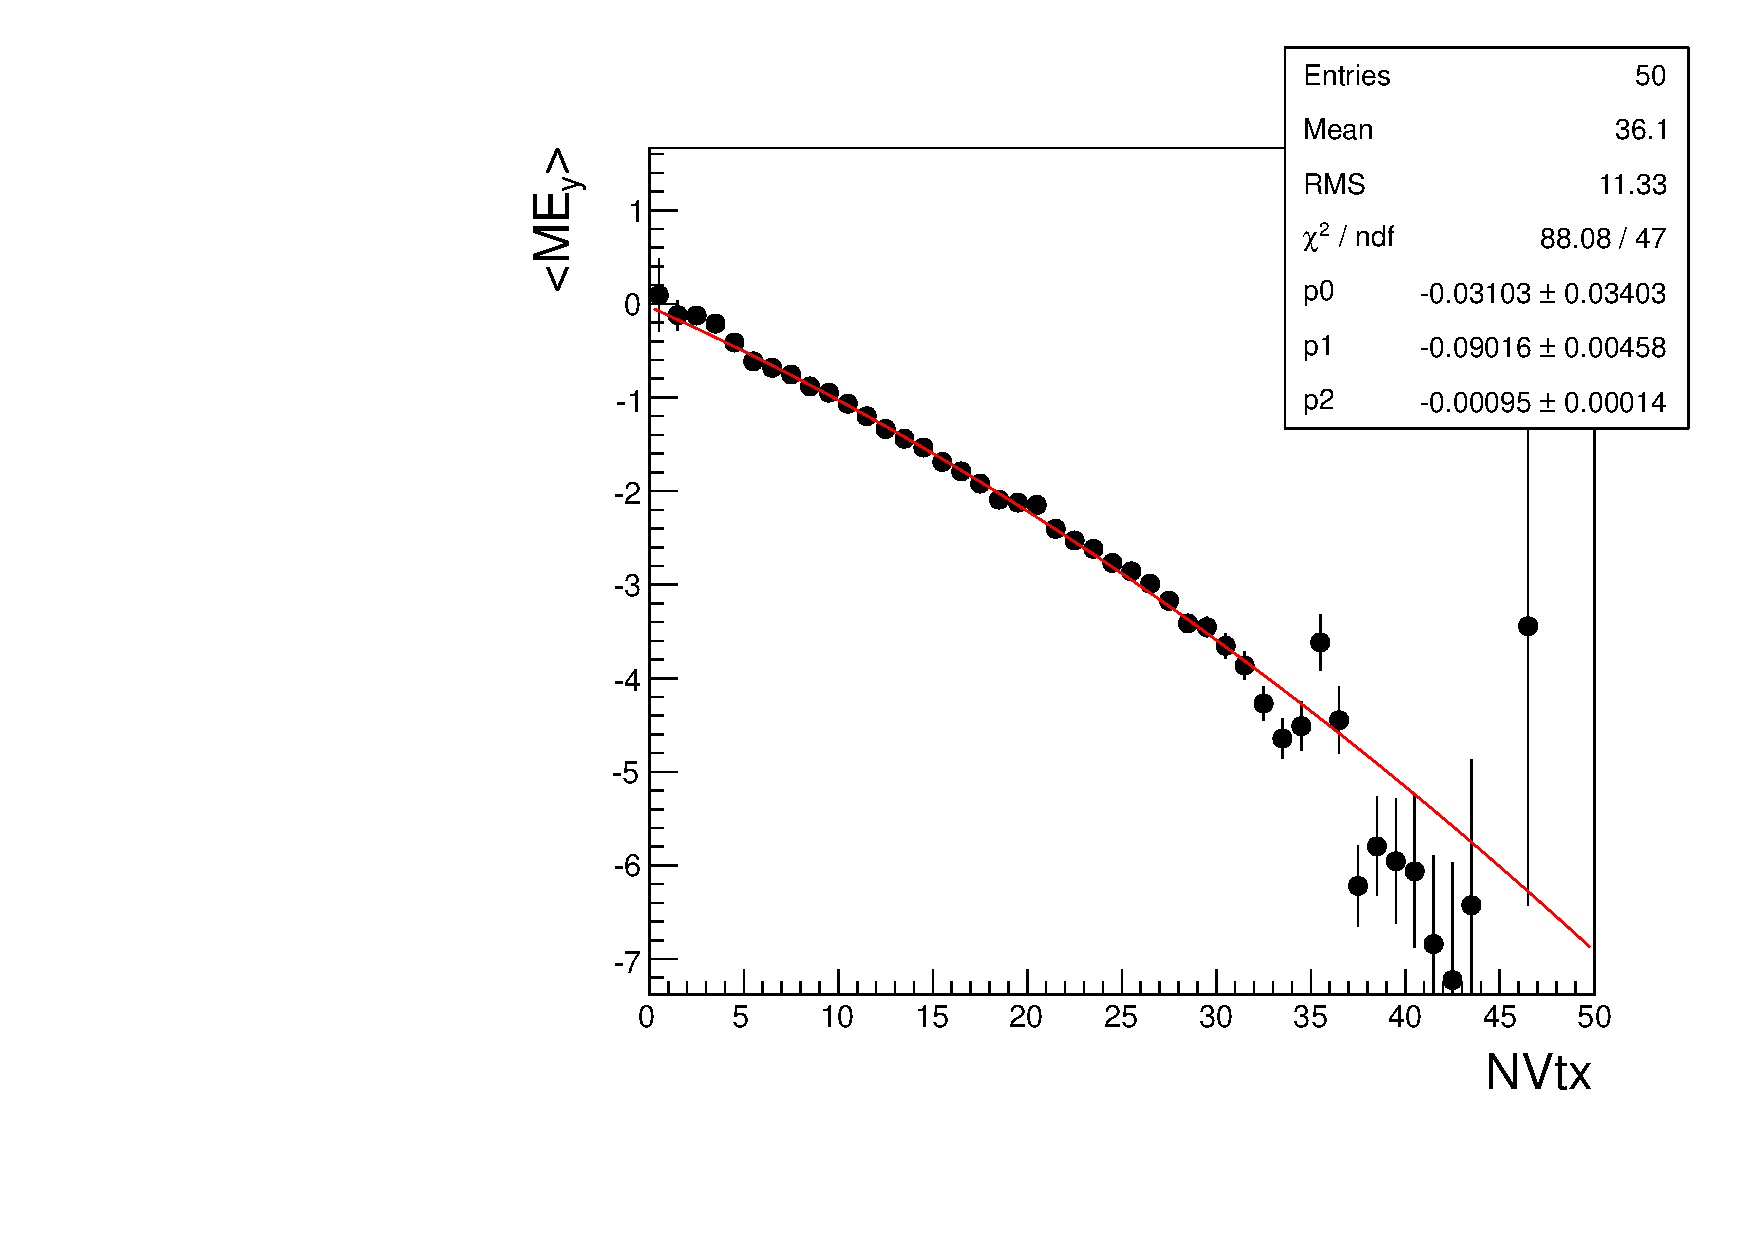
\includegraphics[width=0.45\textwidth]{analysis_figs/linear_fit_mcy.pdf}
    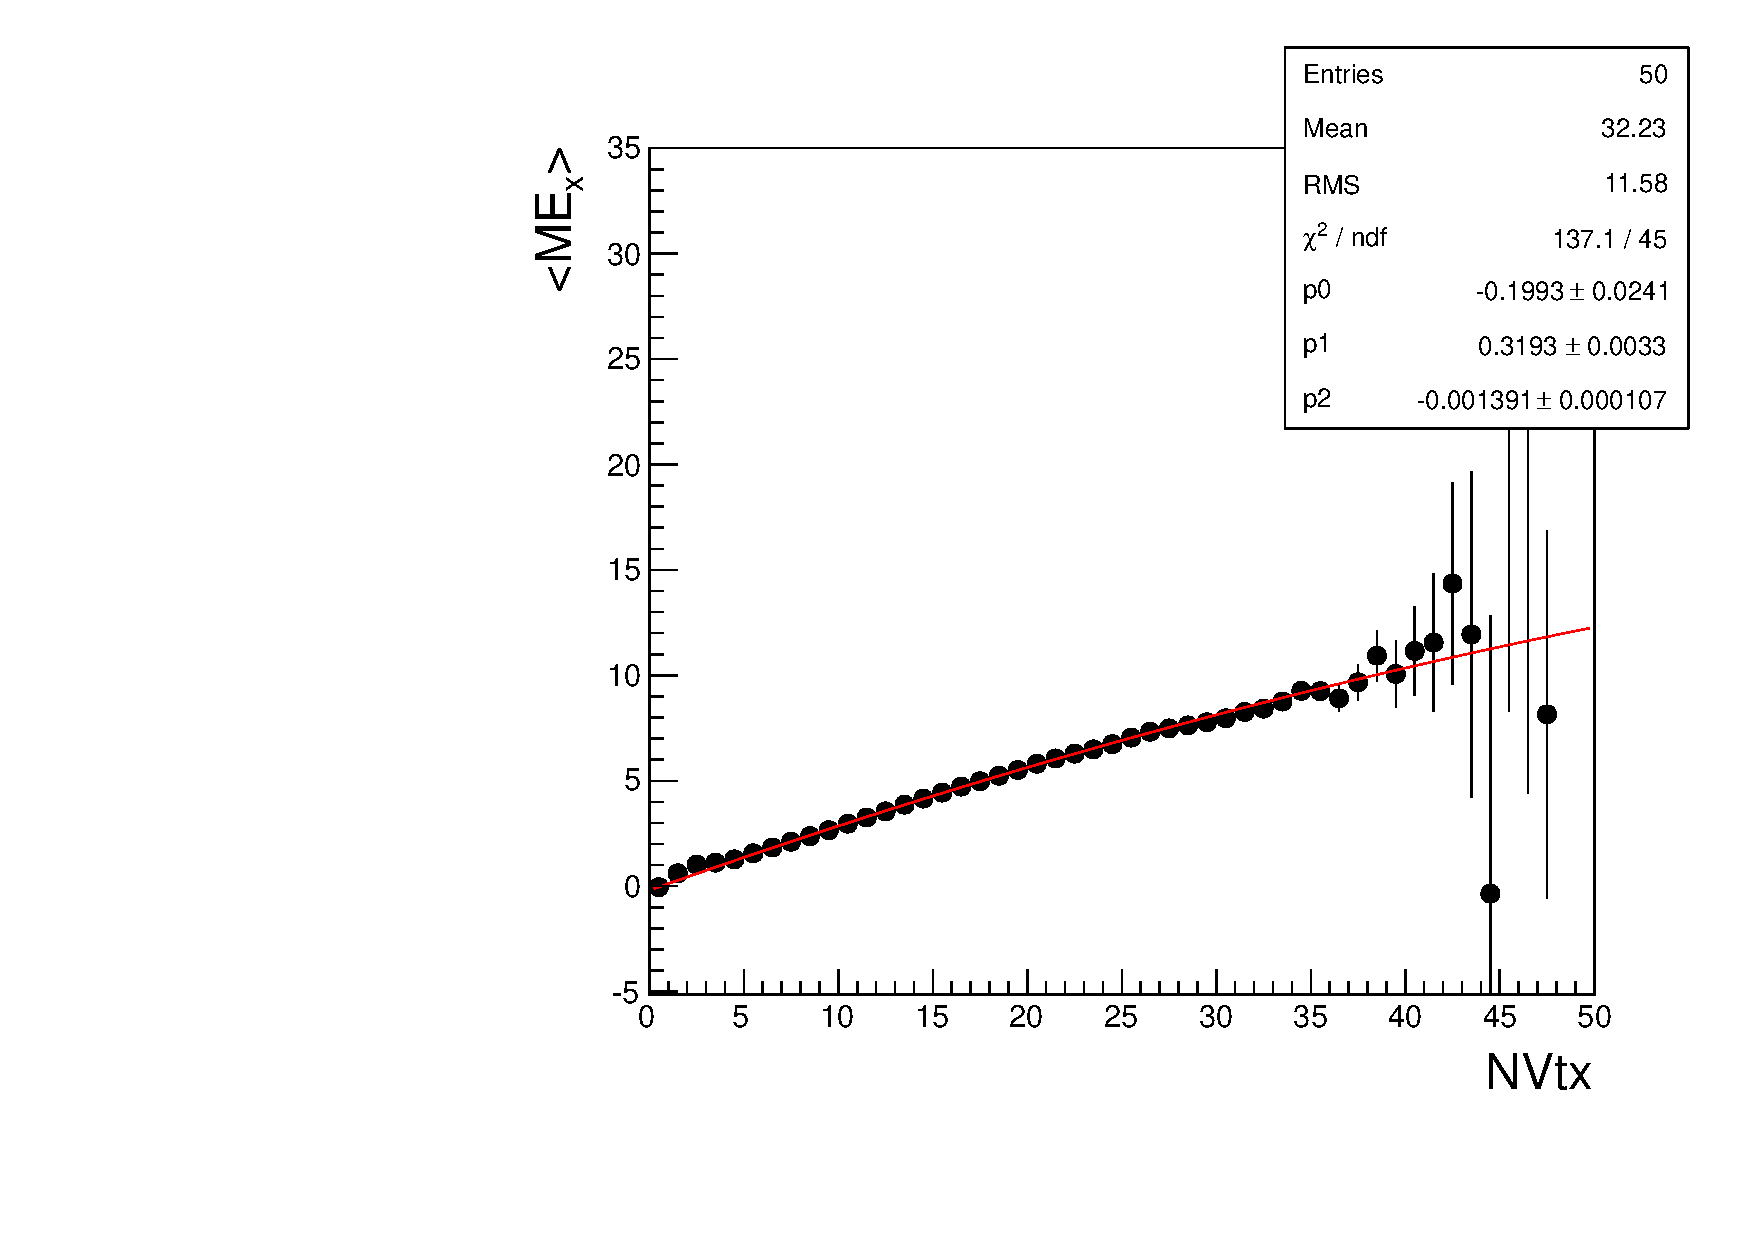
\includegraphics[width=0.45\textwidth]{analysis_figs/linear_fit_datax.pdf}
    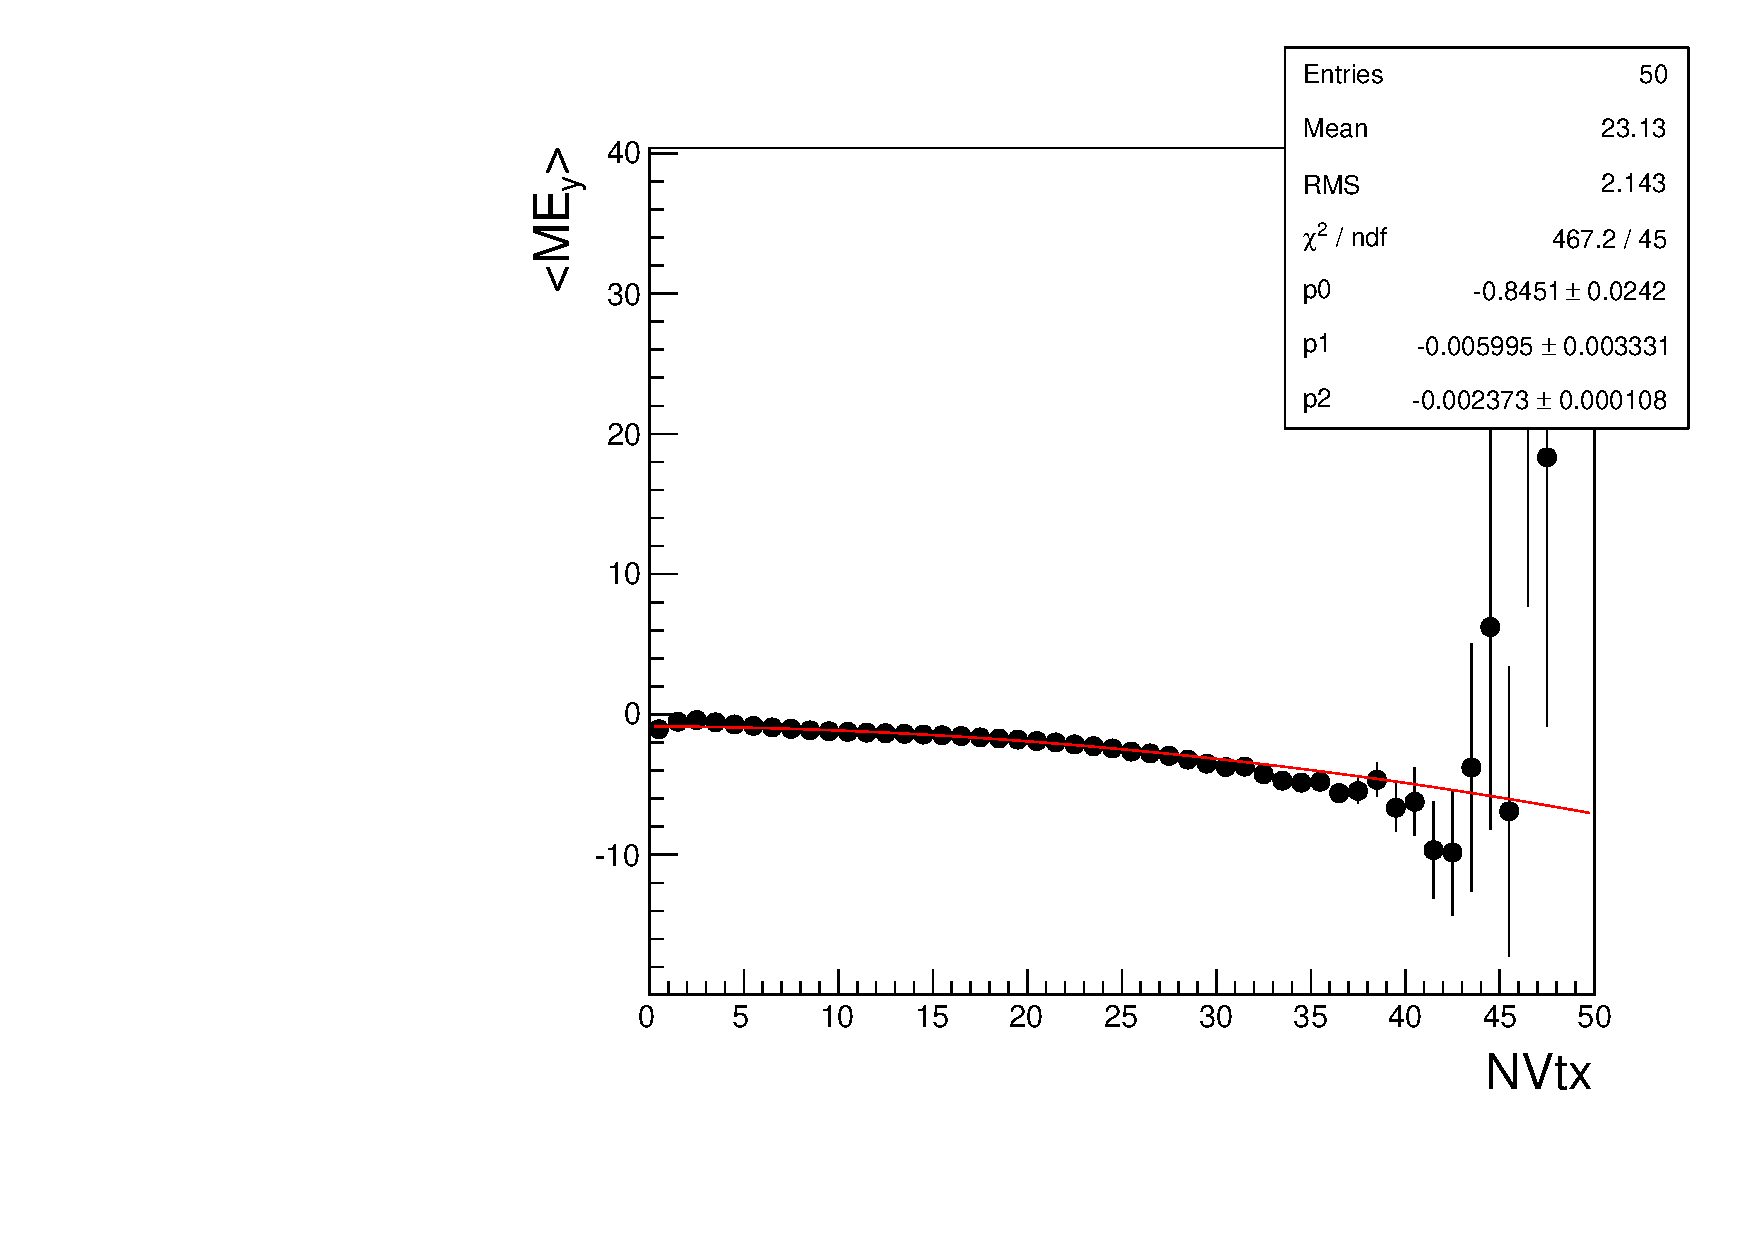
\includegraphics[width=0.45\textwidth]{analysis_figs/linear_fit_datay.pdf}
    \caption{ MET $\phi$ modulation correction fits for all MC (top row), and data (bottom row). }
    \label{fig:metfits}
  \end{center}
\end{figure}

These distributions are fitted with the functional form below, to be able to also account for the changes in the higher and lower number of vertices.

\begin{equation}
\begin{split}
&<\Em_x> = c_{x0} + c_{x1}*N_\mathrm{Vtx} + c_{x2}*N_\mathrm{Vtx}^2  \\
\centering
&<\Em_y> = c_{y0} + c_{y1}*N_\mathrm{Vtx} + c_{y2}*N_\mathrm{Vtx}^2
\end{split}
\end{equation}


The $\Em_x$ and $\Em_y$ are then corrected by:

\begin{equation}
\begin{split}
&\Em_{xcorr} = \Em_x - (c_{x0} + c_{x1}*N_\mathrm{Vtx} + c_{x2}*N_\mathrm{Vtx}^2) \\
&\Em_{ycorr} = \Em_y - (c_{y0} + c_{y1}*N_\mathrm{Vtx} + c_{y2}*N_\mathrm{Vtx}^2)
\end{split}
\end{equation}

The $\phi$ and \met in the event is then recalculated using the corrected $\Em_x$ and $\Em_y$. Fig.~\ref{fig:phicorr} shows the $\phi$ distributions of \met before and after the correction for data, photon+jet sample and inclusive $Z\gamma$ sample.

\begin{figure}[!h]
 \centering
  {\label{fig:a}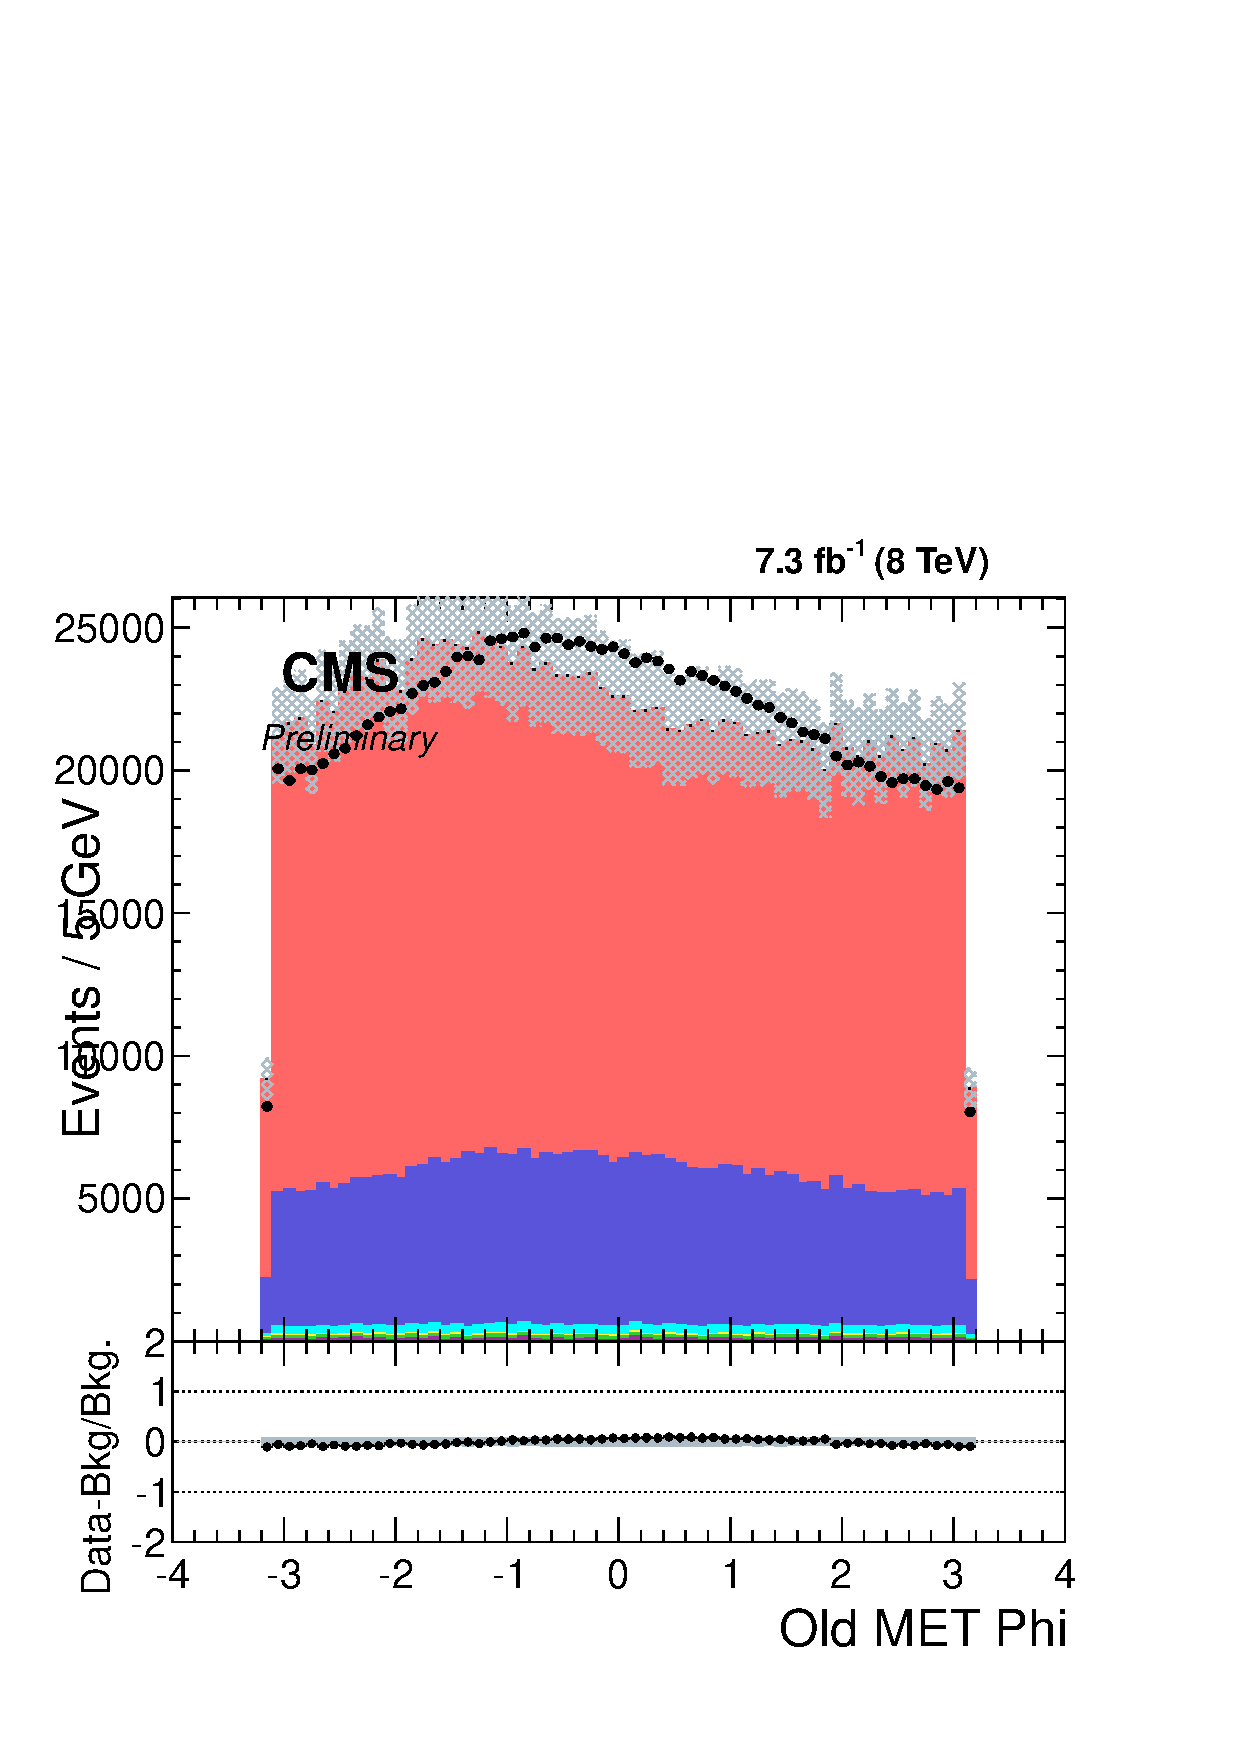
\includegraphics[width=0.45\textwidth]{analysis_figs/before_mphi.pdf}}
  {\label{fig:c}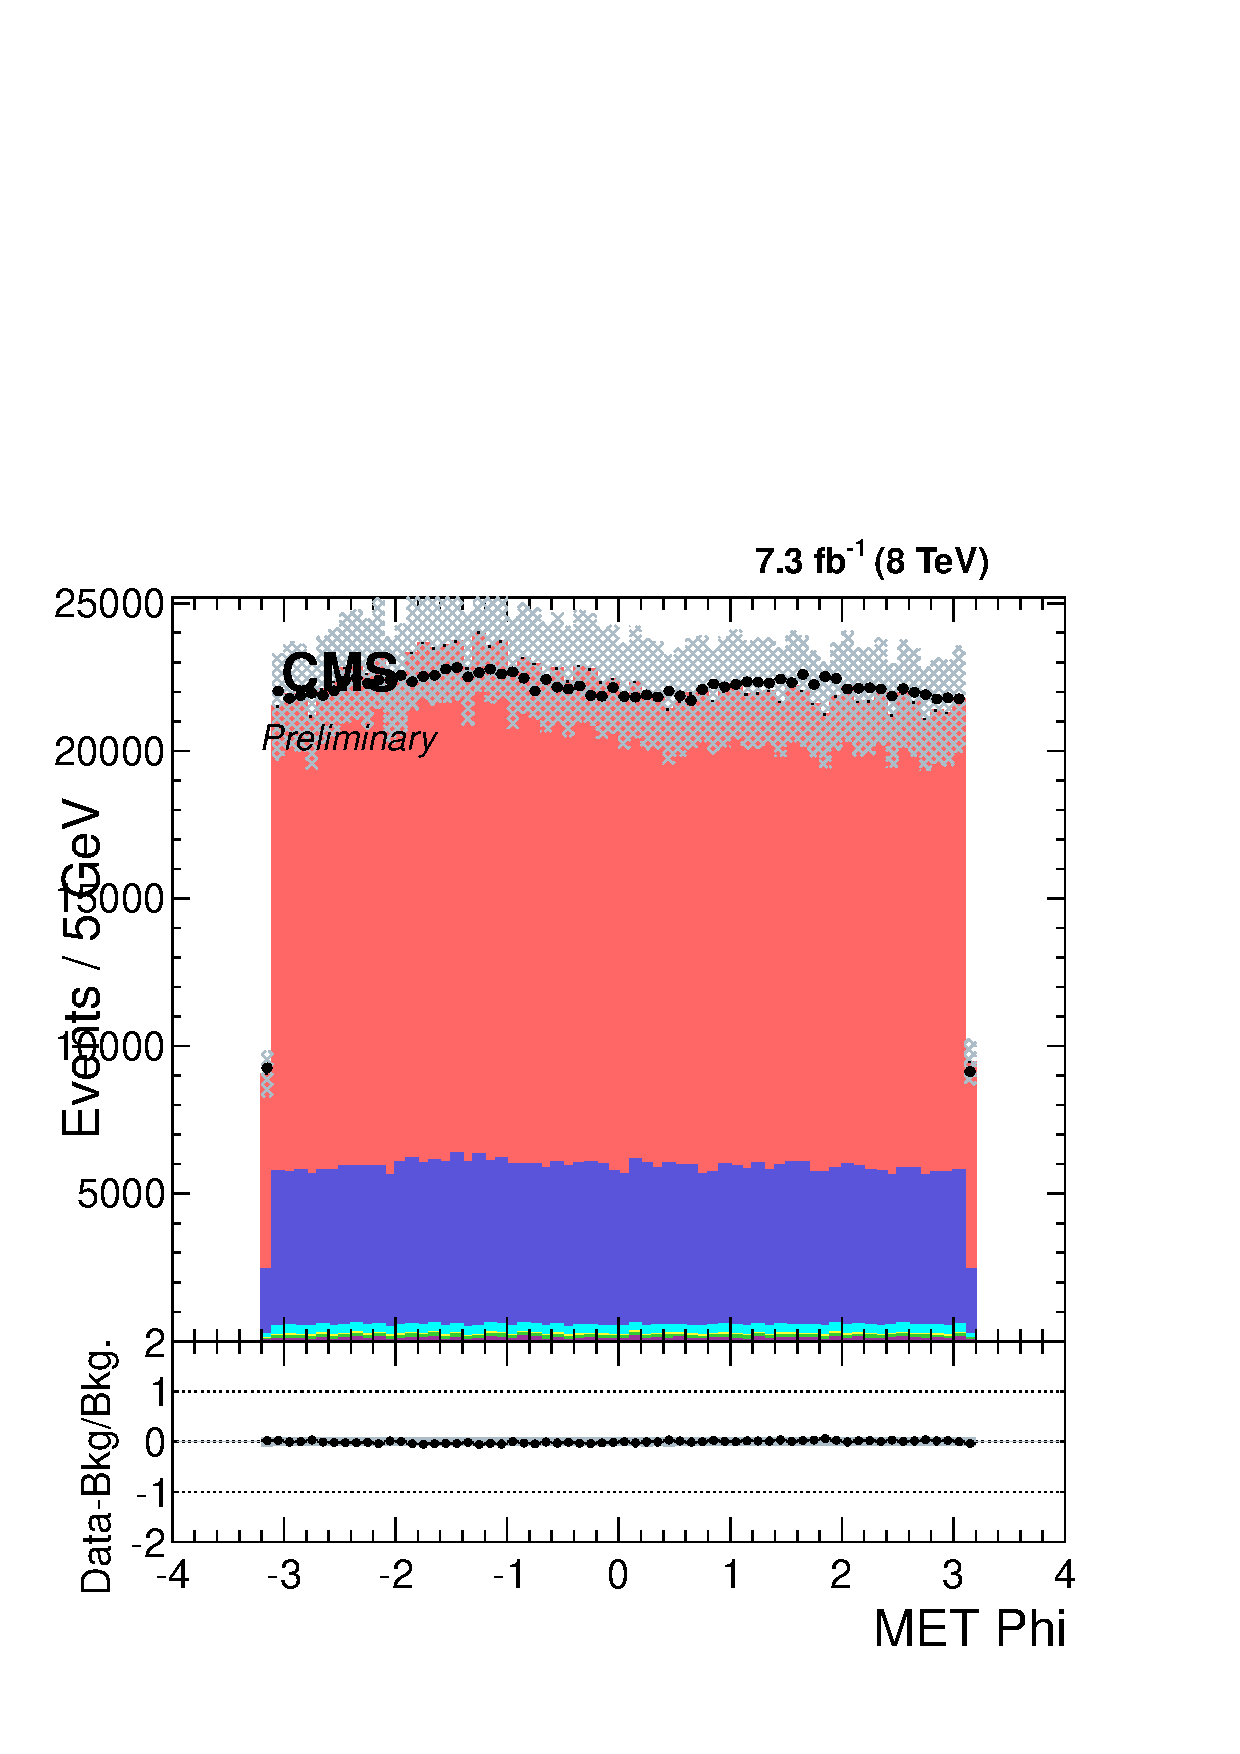
\includegraphics[width=0.45\textwidth]{analysis_figs/after_mphi.pdf}}
 \caption{ $\phi$ distributions before and after the correction in data and mc.}
 \label{fig:phicorr}
\end{figure}

\subsubsection{Fake MET Rejection}
\label{sec:fakemet}
$\gamma + $ jet and dijet processes have large cross section and contribute significatly to the monophoton final state.  These backgrounds do not intrinsically have \met. However, fake \met can arise from many sources, including limited \met resolution, reconstruction inefficiencies, instrumental defects, and improper pattern recognition. In order to minimize the contribution from these processes, we have explored two different methods for identifying events with fake \met. We used the well known \met significance (requiring \met significance $> 20$). By taking into account the reconstructed objects in each event and their known measurement resolutions, the \met significance method provides an event-by-event estimation of the likelihood that the observed \met is consistent with zero ~\cite{Chatrchyan:2011tn}. We further developed our own fake \met method. 

In our method we first construct a $\chi^2$ function with the form:
 
\begin{equation}\label{eq:1a}
   \chi^2 = \sum_{i=objects} \left( \frac{(\PT^{reco})_i-(\widetilde{\PT})_i}{(\sigma_{\PT})_i} \right)^2 + \left( \frac{\widetilde{\Em}_x}{\sigma_{\widetilde{\Em}_x}}\right)^2  + \left( \frac{\widetilde{\Em}_y}{\sigma_{\widetilde{\Em}_y}}\right)^2.
\end{equation} 
In the above equation, $(\PT^{reco})_{i}$ are the transverse  momenta of the reconstructed objects, the $(\sigma_{\PT})_{i}$ are the expected resolutions of each object, and the
$(\widetilde{p}_{\mathrm T})_{i}$ are the free parameters allowed to vary in order to minimize the function. Furthermore, $\Em_x$ and $\Em_y$ can be expressed as:
  
%\begin{equation}
% \Em^{reco}_{x,y} + \sum_{i=objects} (p_{x,y}^{reco})_i-(\widetilde{p}_{x,y})_i  = - \sum_{i=objects} (\widetilde{p}_{x,y})_i
%\end{equation}

\begin{equation}
\begin{split}
\widetilde{\Em}_{x,y} &=  \underbrace{\Em^{reco}_{x,y} + \sum_{i=objects} (p_{x,y}^{reco})_i}_\text{=0} - (\widetilde{p}_{x,y})_i \\
\widetilde{\Em}_{x,y} &=  - \sum_{i=objects} (\widetilde{p}_{x,y})_i
\end{split}
\end{equation}


To understand better the above equations, let us look at an extreme condition. 
\begin{itemize}
\item Assume an event with no-intrinsic \met i.e., $\met = -\sum_{i=objects} p_{T,i} = 0$. Then by construction, the $\widetilde{\PT}_i$ will be set to $p_{T,i}$ . Given that $-\widetilde{p}_{T,i} = - p_{T,i} = 0$, these types of events will be cut out by the PFMET selection.
\item Now, assume an event with no intrinsic \met but with some observed \met. This situation implies that some of the objects in the event is mismeasured. This time, the method, through a multi-dimentional scan of $\widetilde{\PT}_i$ parameters, will try to minimize the $\widetilde{\met}$ by trying to assign the observed $\met$ back into $\widetilde{\PT}_i$ parameters. If this balancing is done easily than the we will end up with a low $\chi^{2}$ value (with a high probability). These types of events are aimed to be rejected.
\item Lasty in the case of intrinsic \met and observed \met, the minimization of the $\widetilde{\met}$ will not be easy (as there would be no combination of $\widetilde{\PT}_i$ parameters to reduce the \met), therefore will result in high $\chi^2$ and low probability values. 
\end{itemize}
%In events with no intrinsic \met, the unclustered energy will be more easily re-distributed back into the object momenta which will result in a low $\chi^{2}$ value. On the other hand, in events with intrinsic \met, minimization of the $\chi^{2}$ function will be more difficult and will result in larger $\chi^{2}$ values. To reduce the contribution of events with non-intrinsic \met, the probability value obtained from the $\chi^{2}$ minimization  and the recalculated \met~ (i.e., where the original PF candidate $\PT$'s are replaced with their $\widetilde{p}_{\mathrm T}$ obtained from the $\chi^{2}$ minimization) are used as discriminators.

All the visible objects in the hard scattering event (passing event/object selection requirements) are used in this minimization method. In explicitly, all jets that have not been identified as pile up jets, with $\pt > 30 \GeV$ and that do not overlap with a photon or a lepton are used in this minimization. Good electrons and muons that are not overlapping with a photon and with $\pt > 10 \GeV$ are also used in the minimization. 

Assignment of the momentum measurement uncertainties is an important aspect of this technique. These uncertainties are needed in Eq.~\ref{eq:1a} to be able to weight the particle momenta according to its resolution. The object that has the poorest resolution are the jets; therefore ${\met}$ resolution is dominated by jets. This means that the dominant source of  fake ${\met}$  will be mis-measured jets. The jet resolution is measured by the JetMET POG using the dijet pT asymmetry distributions and the photon+jet balancing technique. The resolution as a function of transverse momentum is given in 12 different $\eta$ ranges as shown in Fig. \ref{fig:FIT1} and \ref{fig:FIT2}. The resolution difference in data and MC is also taken into account and scale factors are provided in Table \ref{jet_table}. The functional form used to parameterize the resolution, introduced to describe the resolution of particle flow jets is \cite{jetreso}:

\begin{equation}\label{eq:jetreso}
JER = \sqrt{\left(\frac{N}{\PT}\right)^2 + S^2 \PT^{m-1} + C^2 } 
\end{equation}
where, $N$ refers to the noise, $S$ to the stocastic, and $C$ to the constant term. The additional parameter $m$ is introduced, to improve the fits to the jet $p_T$ resolution vs. $p_T$.


% Add JET RESOLUTION PLOTS HERE WITH THE SCALE FACTOR TABLE

\begin{figure}[!h]
 \centering
  {\label{fig:fit1a}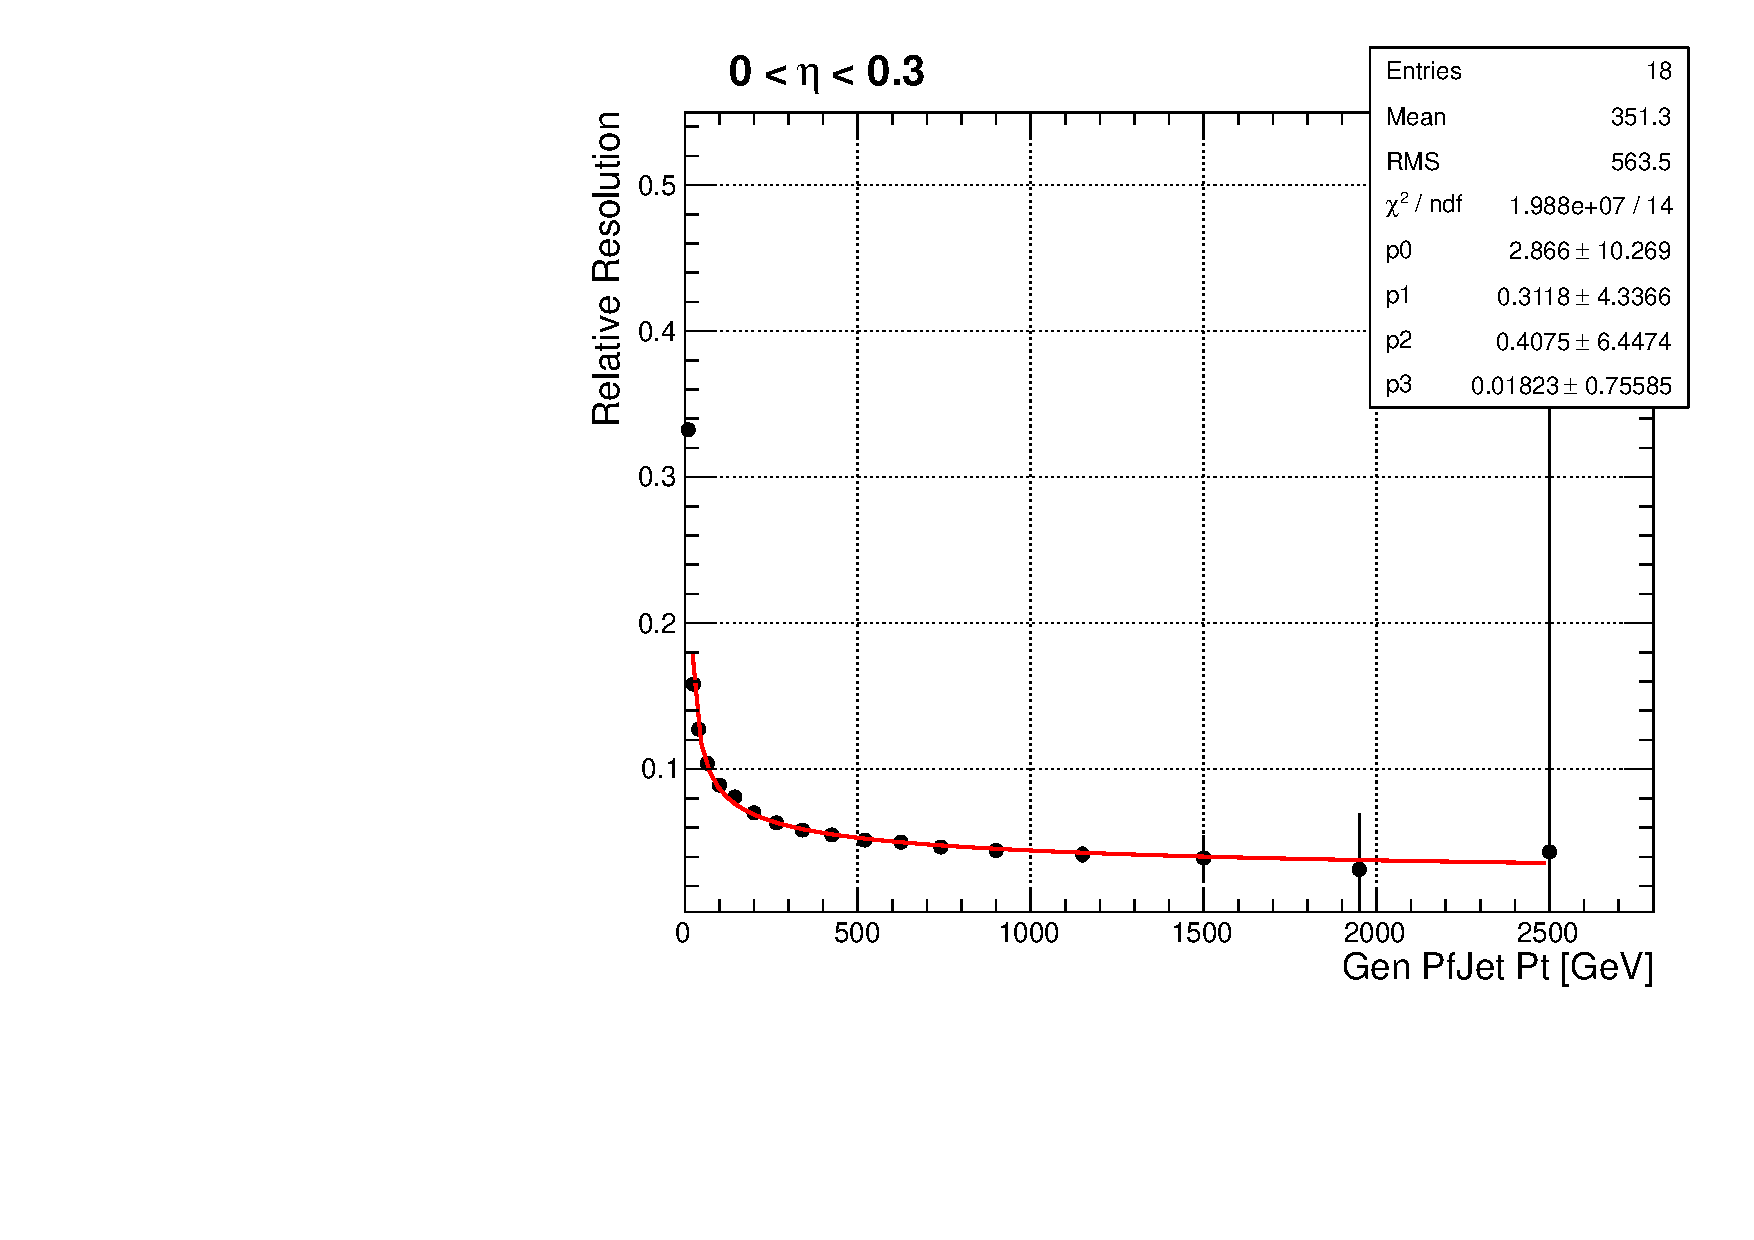
\includegraphics[width=5.3cm,height=5.3cm]{analysis_figs/eta0.pdf}}
  {\label{fig:fit1b}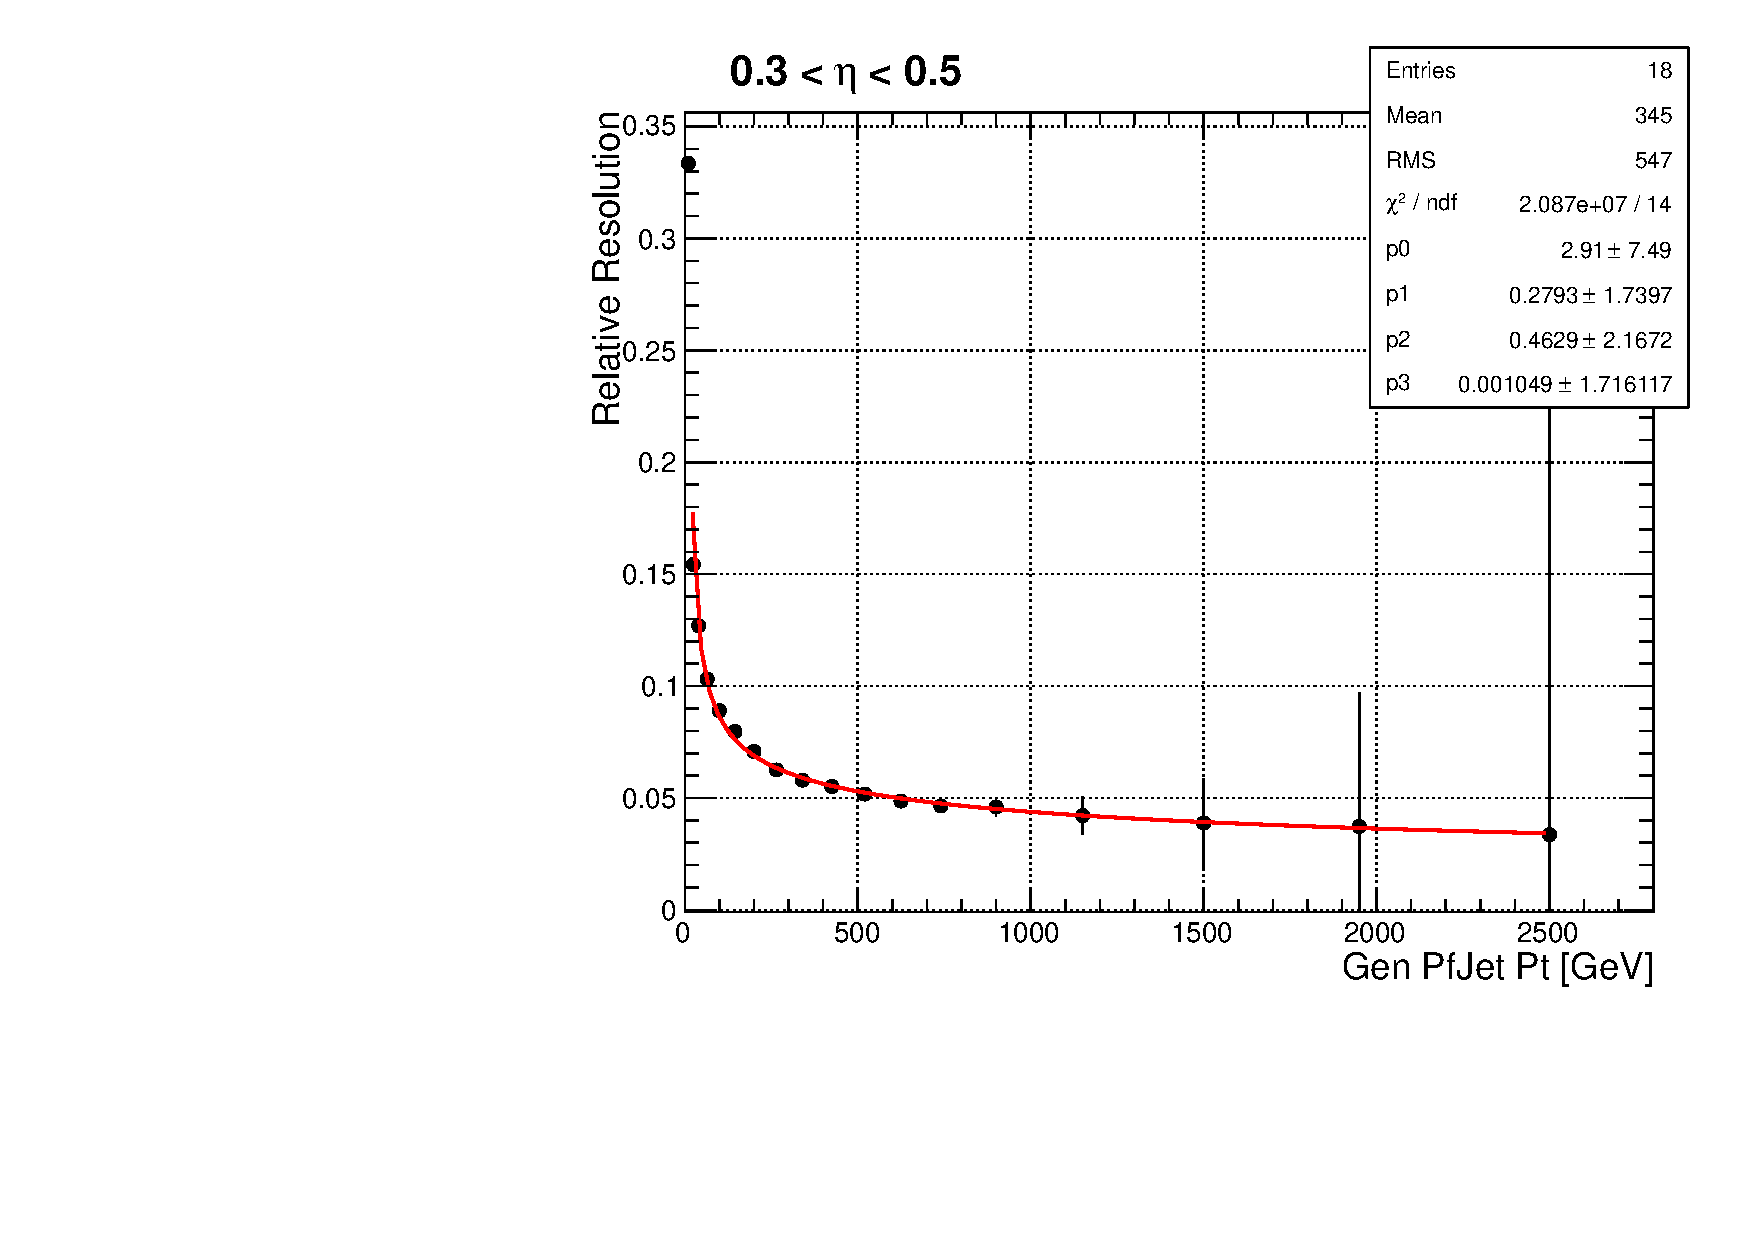
\includegraphics[width=5.3cm,height=5.3cm]{analysis_figs/eta1.pdf}} 
  {\label{fig:fit1c}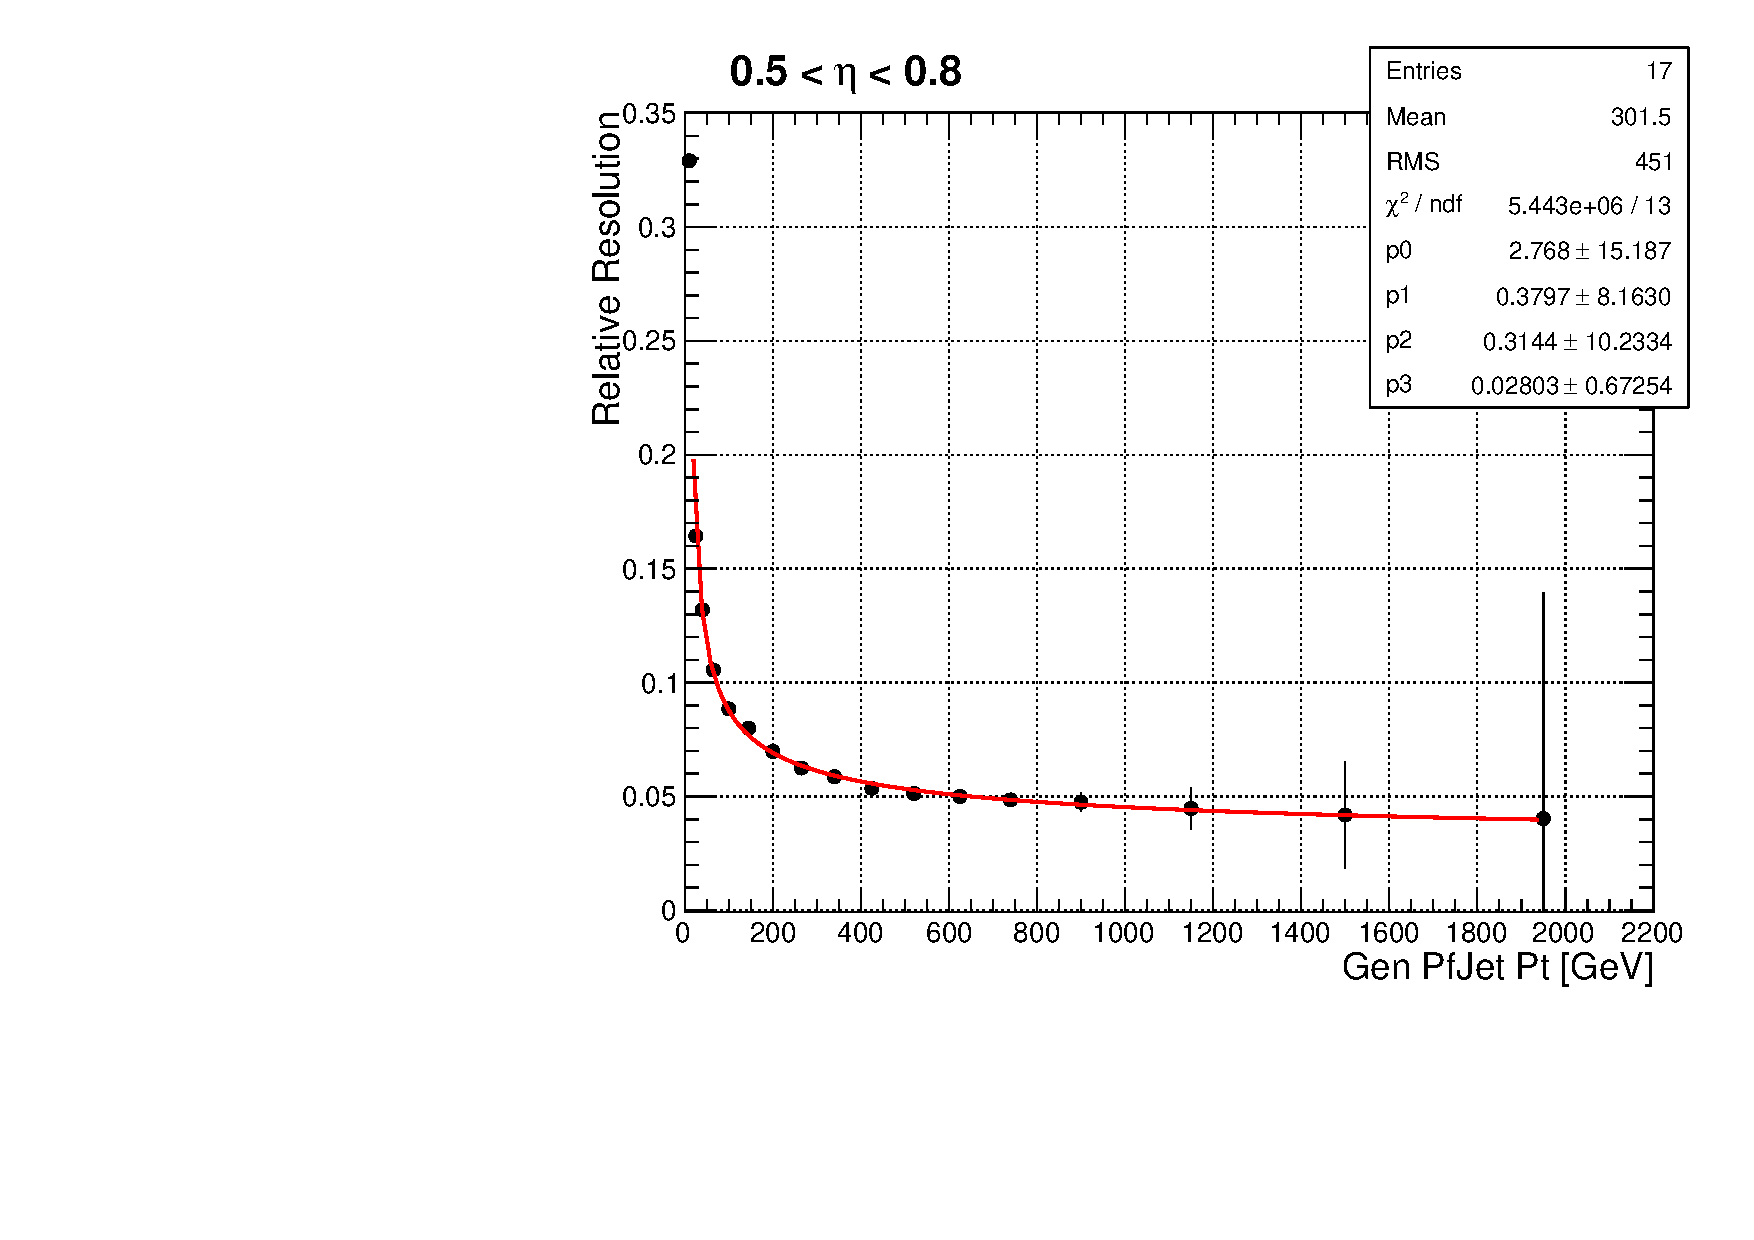
\includegraphics[width=5.3cm,height=5.3cm]{analysis_figs/eta2.pdf}} \\
  {\label{fig:fit1d}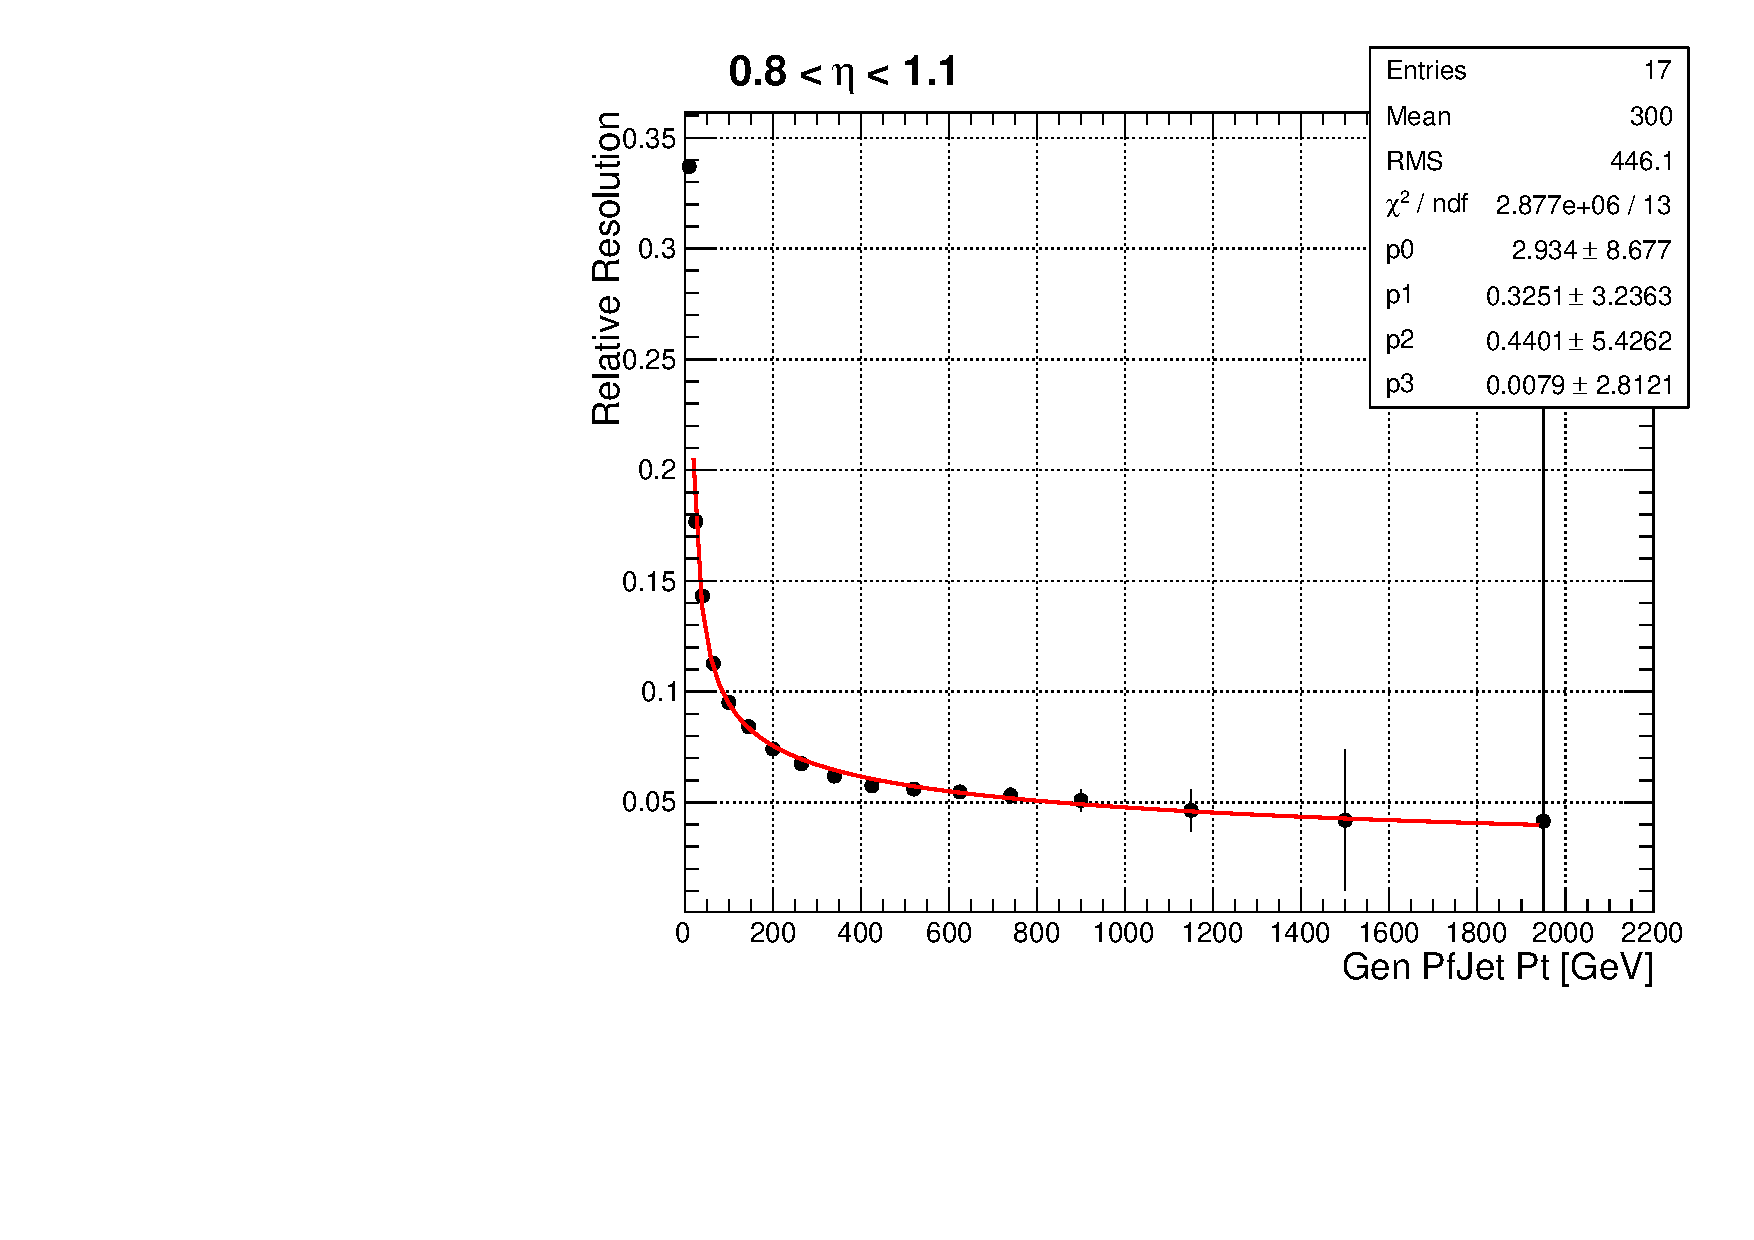
\includegraphics[width=5.3cm,height=5.3cm]{analysis_figs/eta3.pdf}} 
  {\label{fig:fit1e}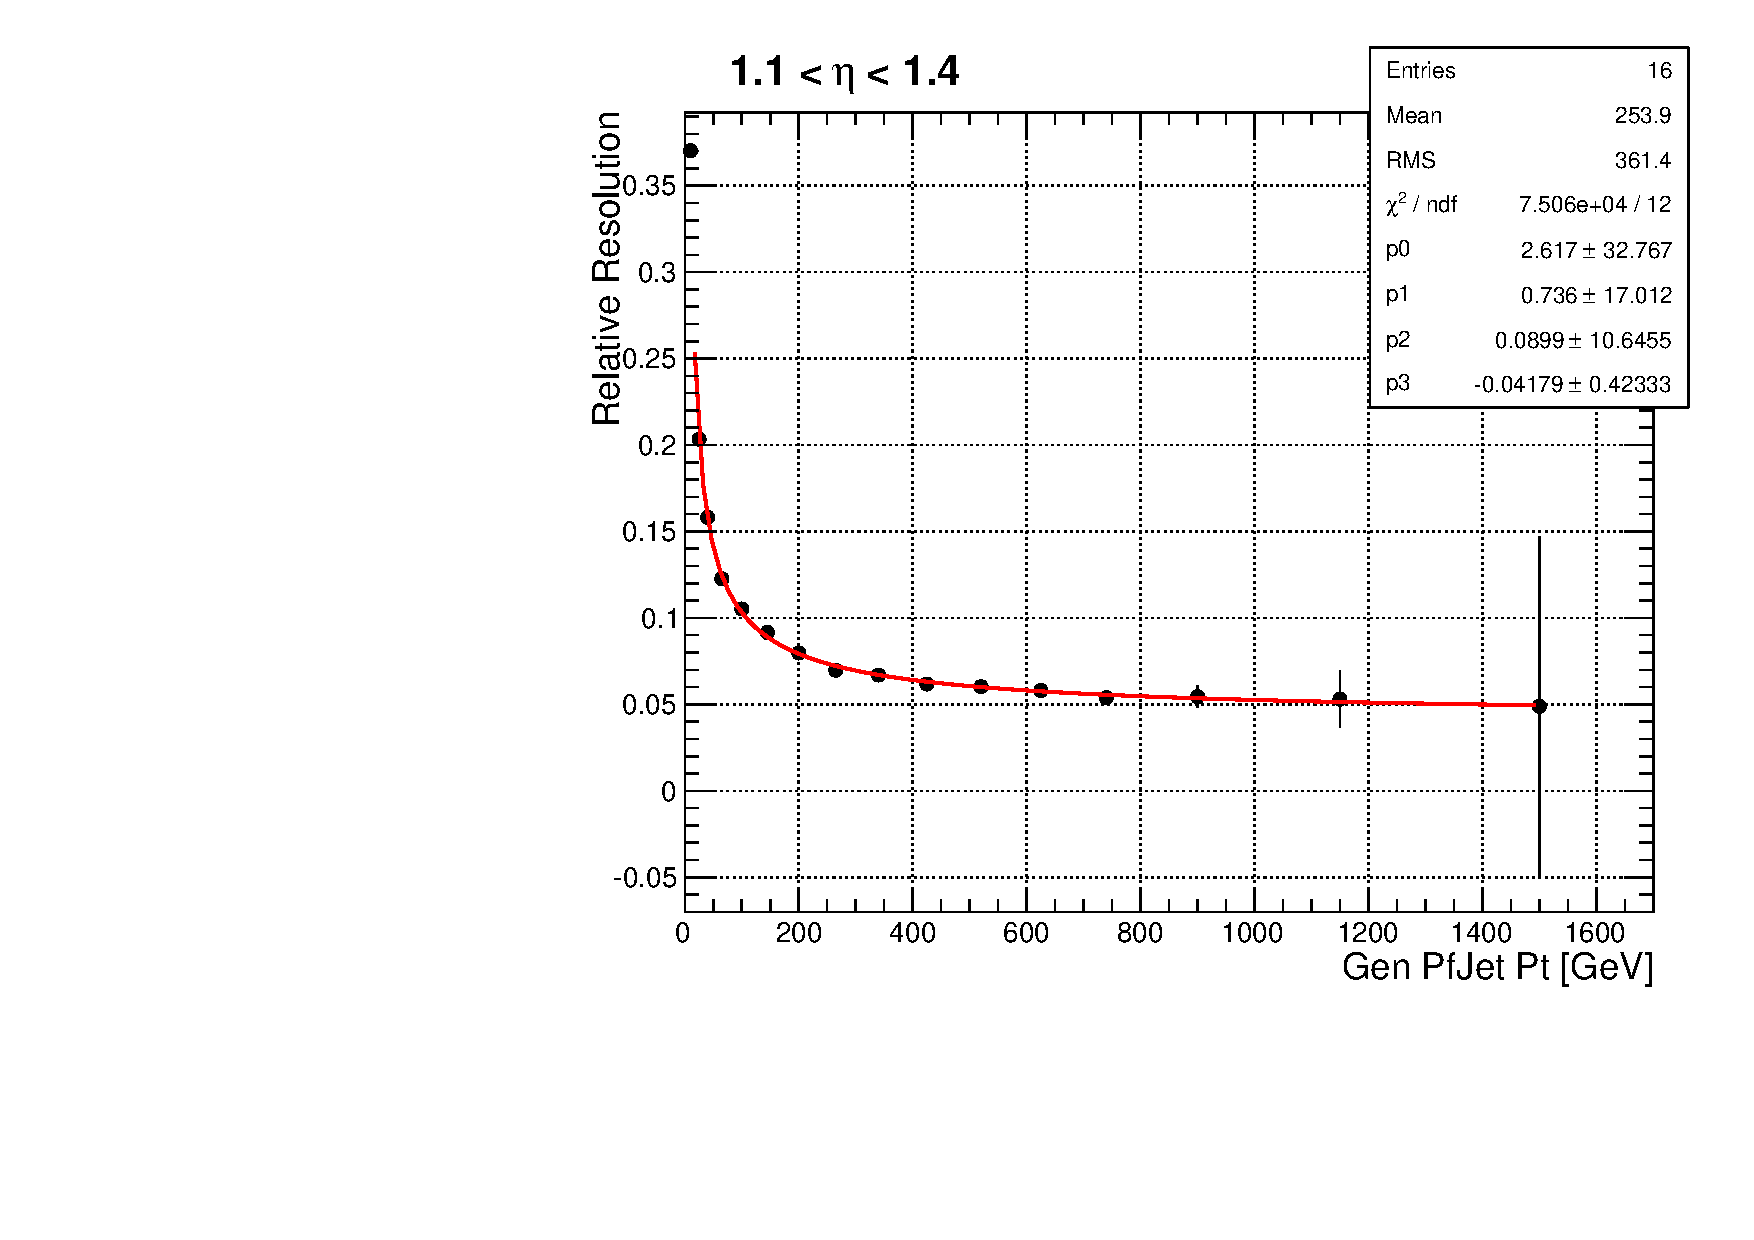
\includegraphics[width=5.3cm,height=5.3cm]{analysis_figs/eta4.pdf}}
  {\label{fig:fit1f}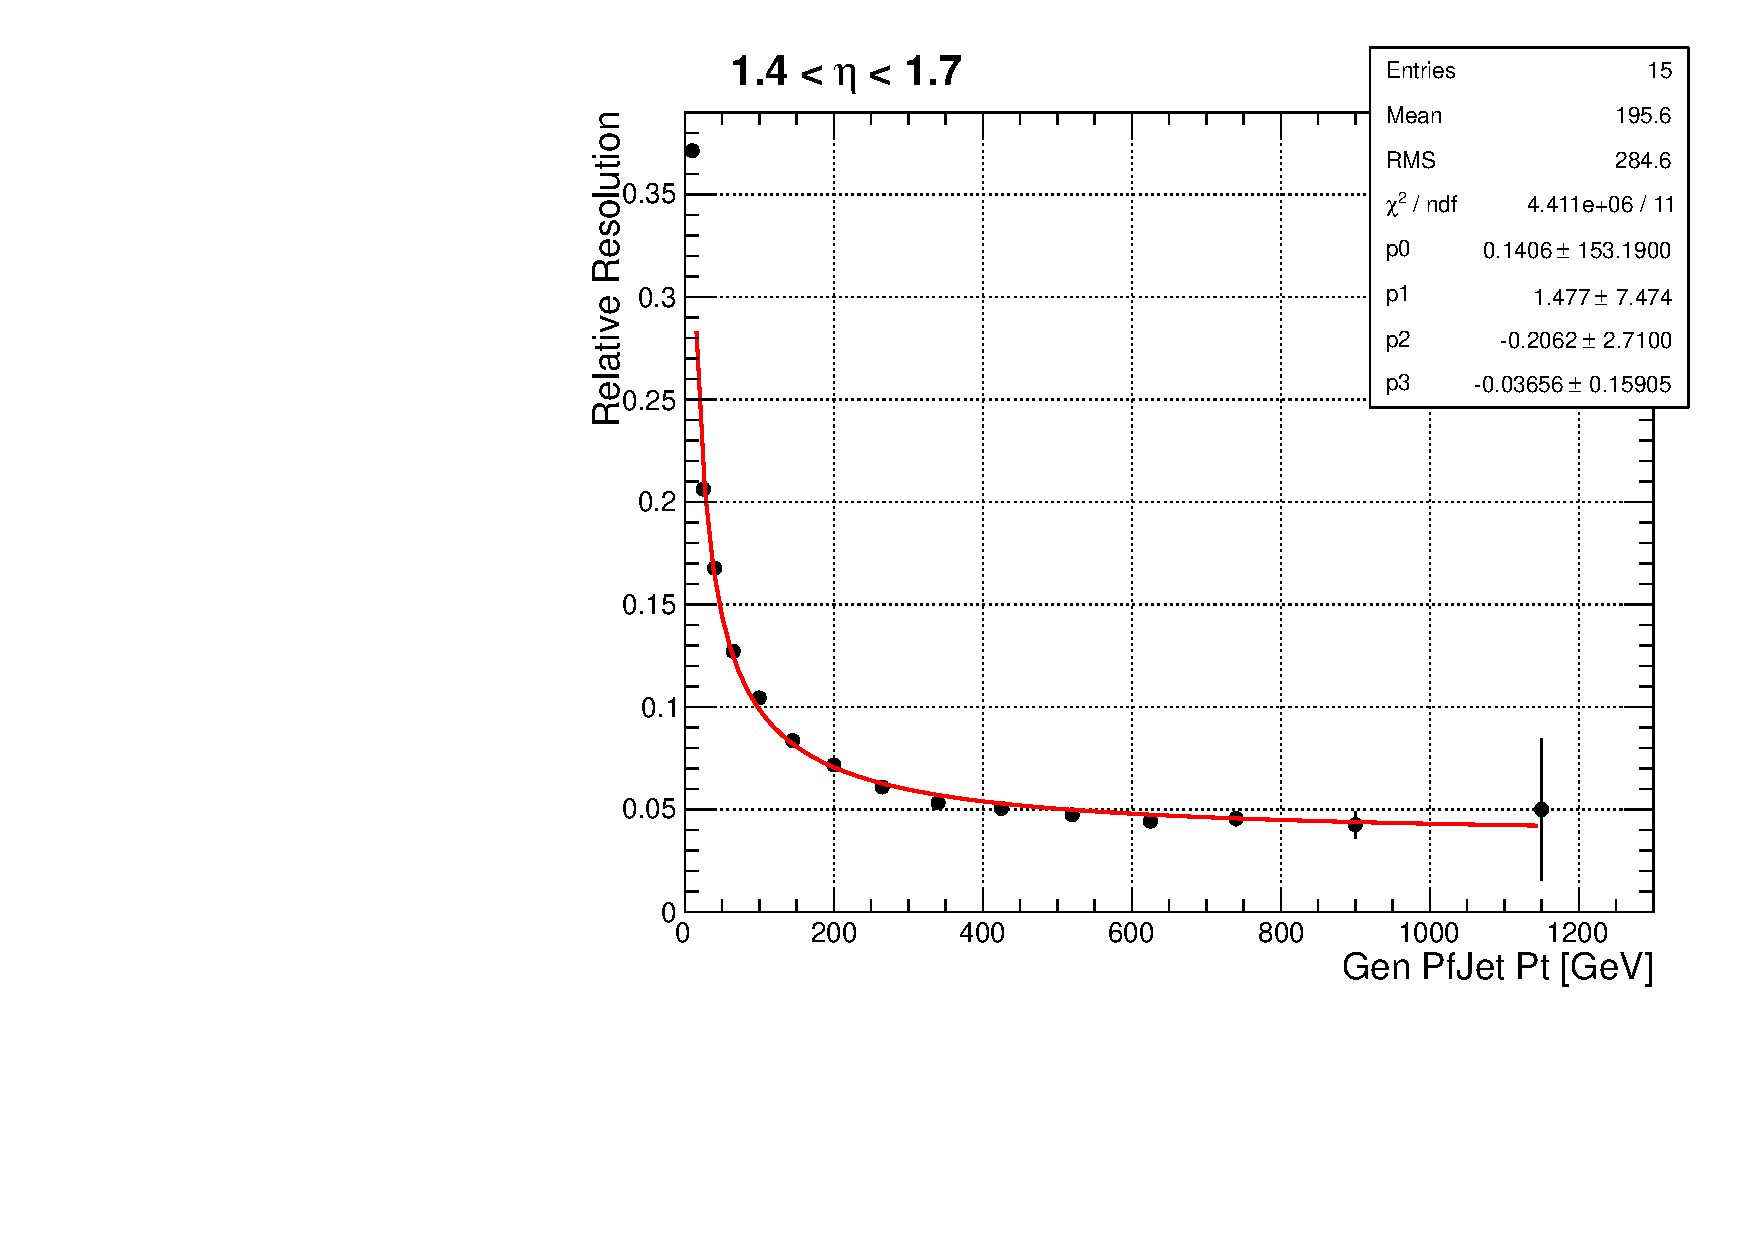
\includegraphics[width=5.3cm,height=5.3cm]{analysis_figs/eta5.pdf}} 
 \caption{ The jet transverse momentum resolution as a function of transverse momentum is given in 12 different $\eta$ ranges}
\label{fig:FIT1}
\end{figure}     

\begin{figure}[!h]
 \centering
  {\label{fig:fit2a}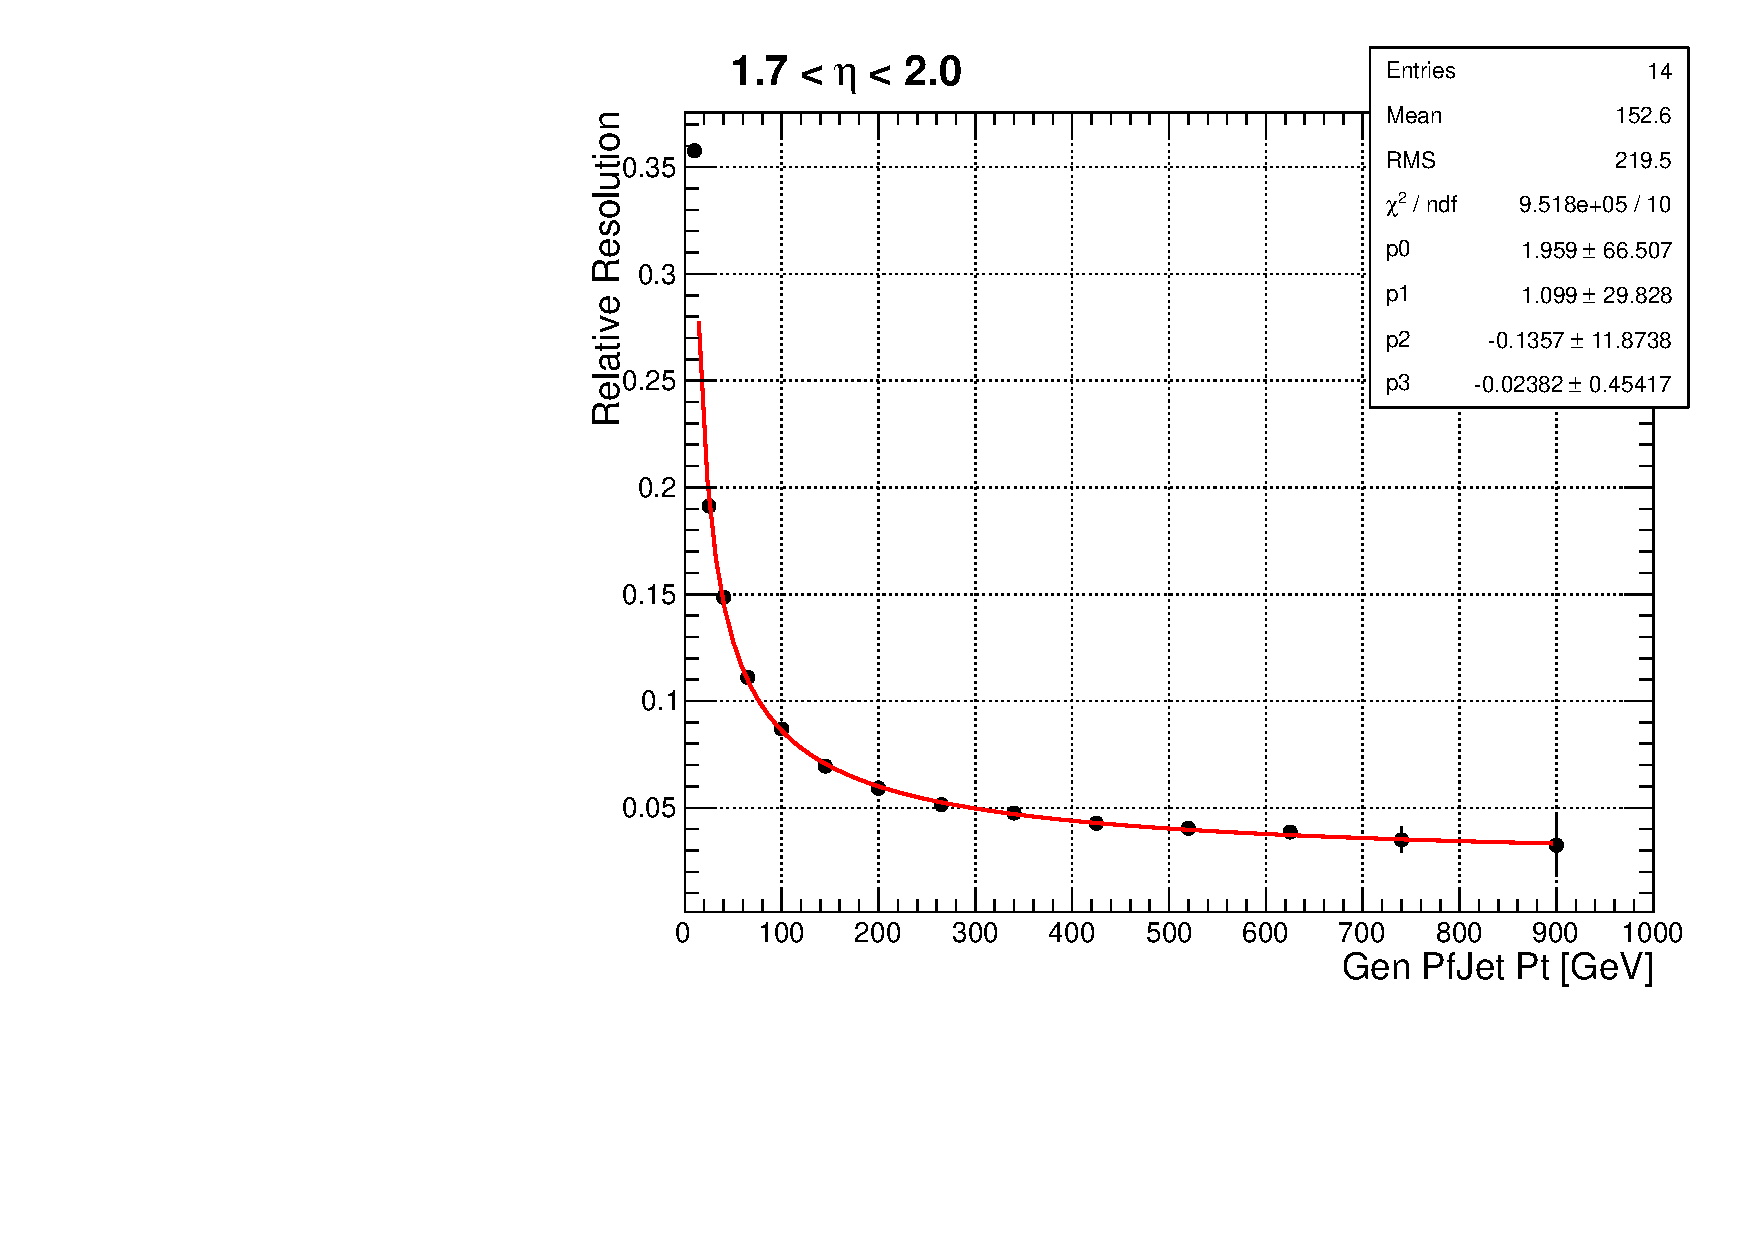
\includegraphics[width=5.3cm,height=5.3cm]{analysis_figs/eta6.pdf}}
  {\label{fig:fit2b}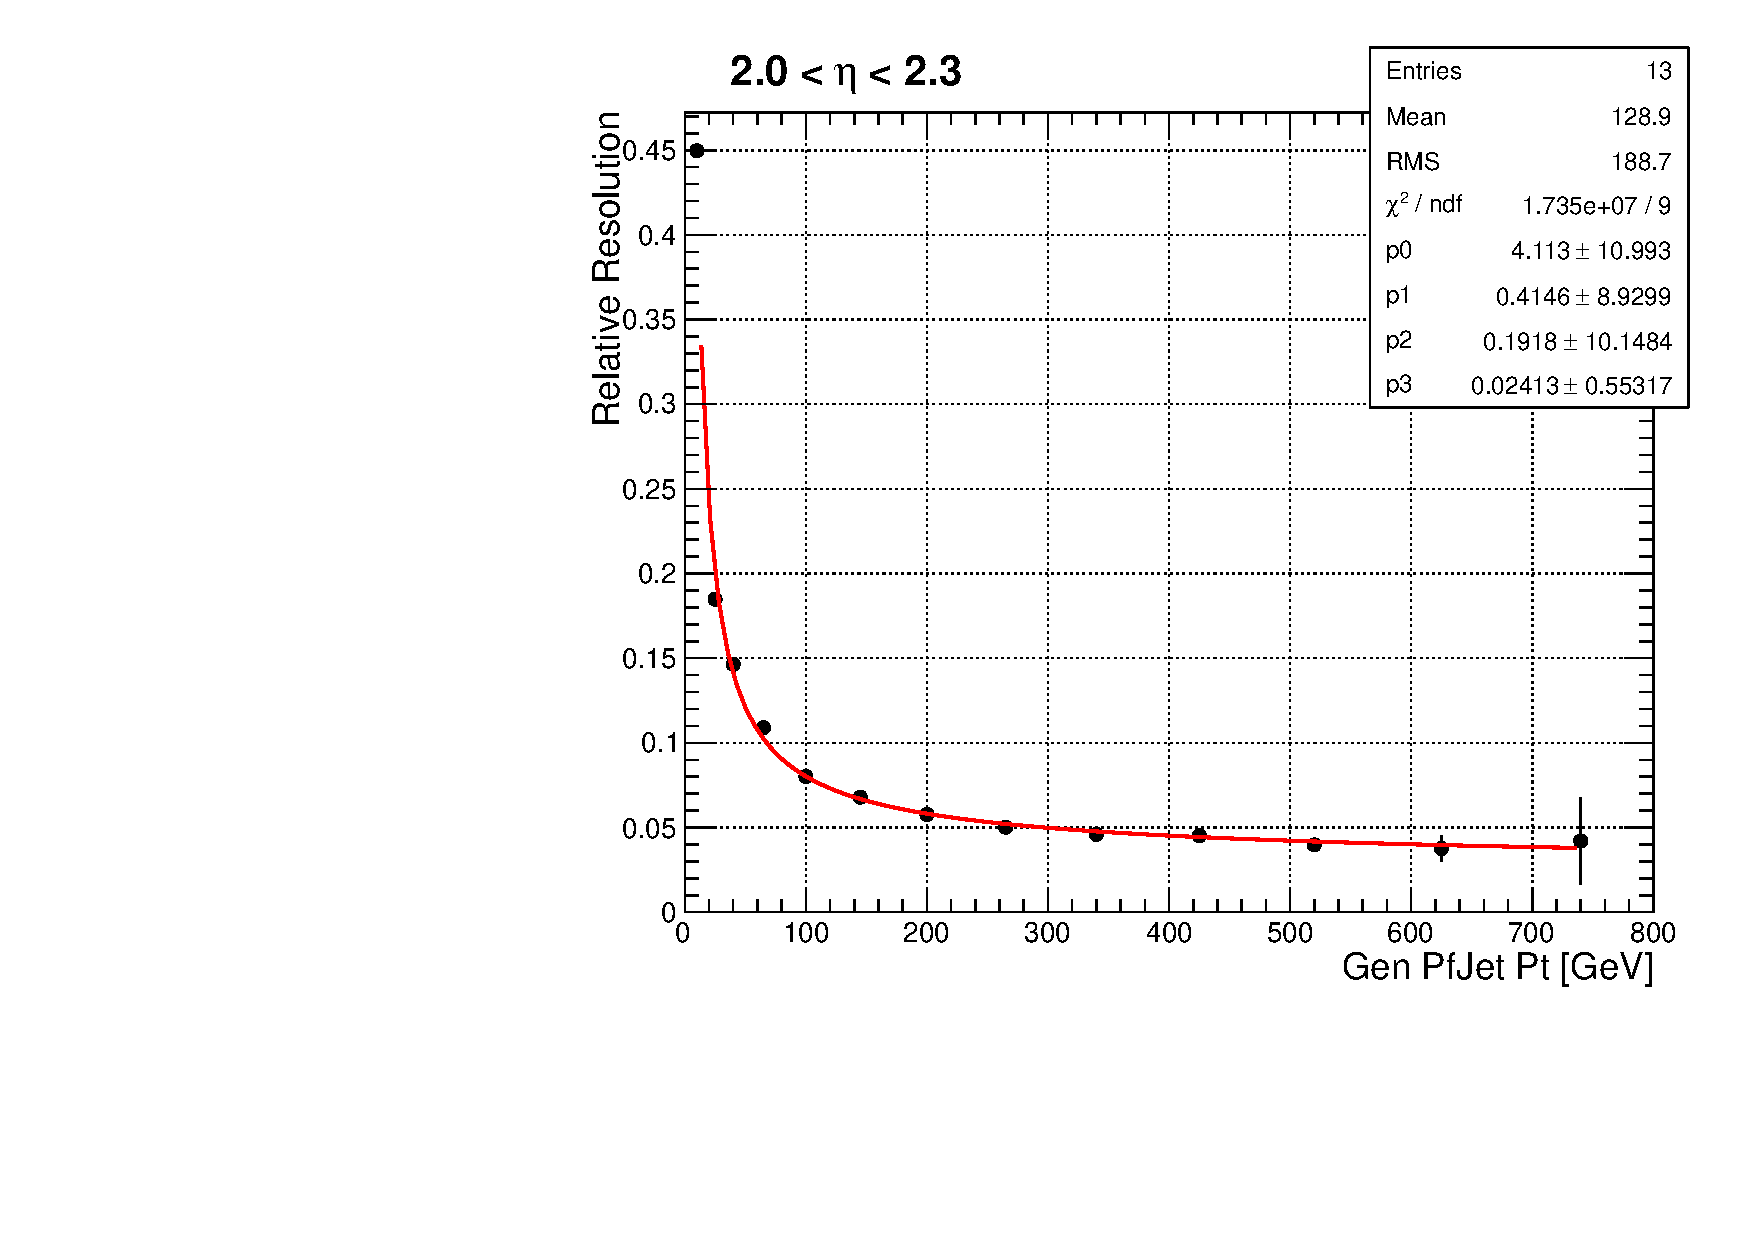
\includegraphics[width=5.3cm,height=5.3cm]{analysis_figs/eta7.pdf}} 
  {\label{fig:fit2c}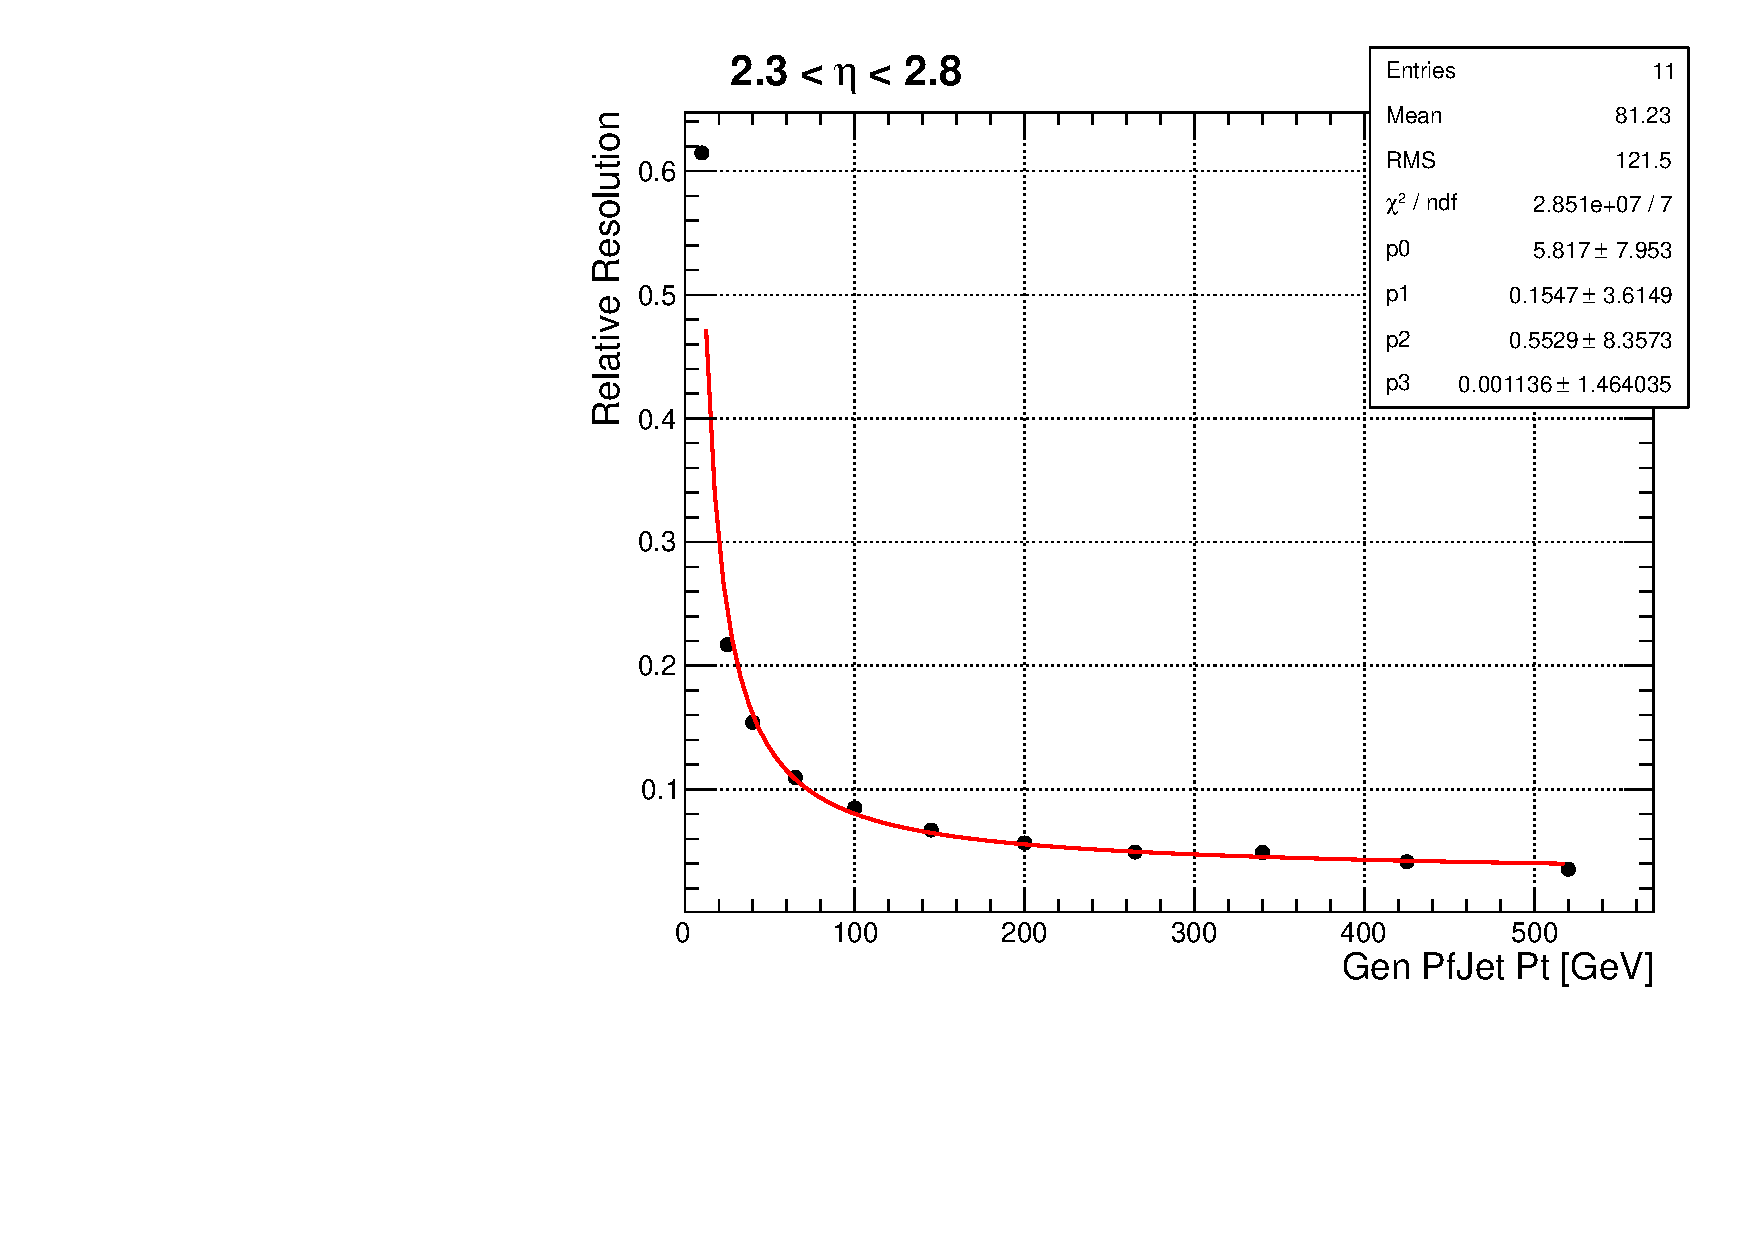
\includegraphics[width=5.3cm,height=5.3cm]{analysis_figs/eta8.pdf}} \\
  {\label{fig:fit2d}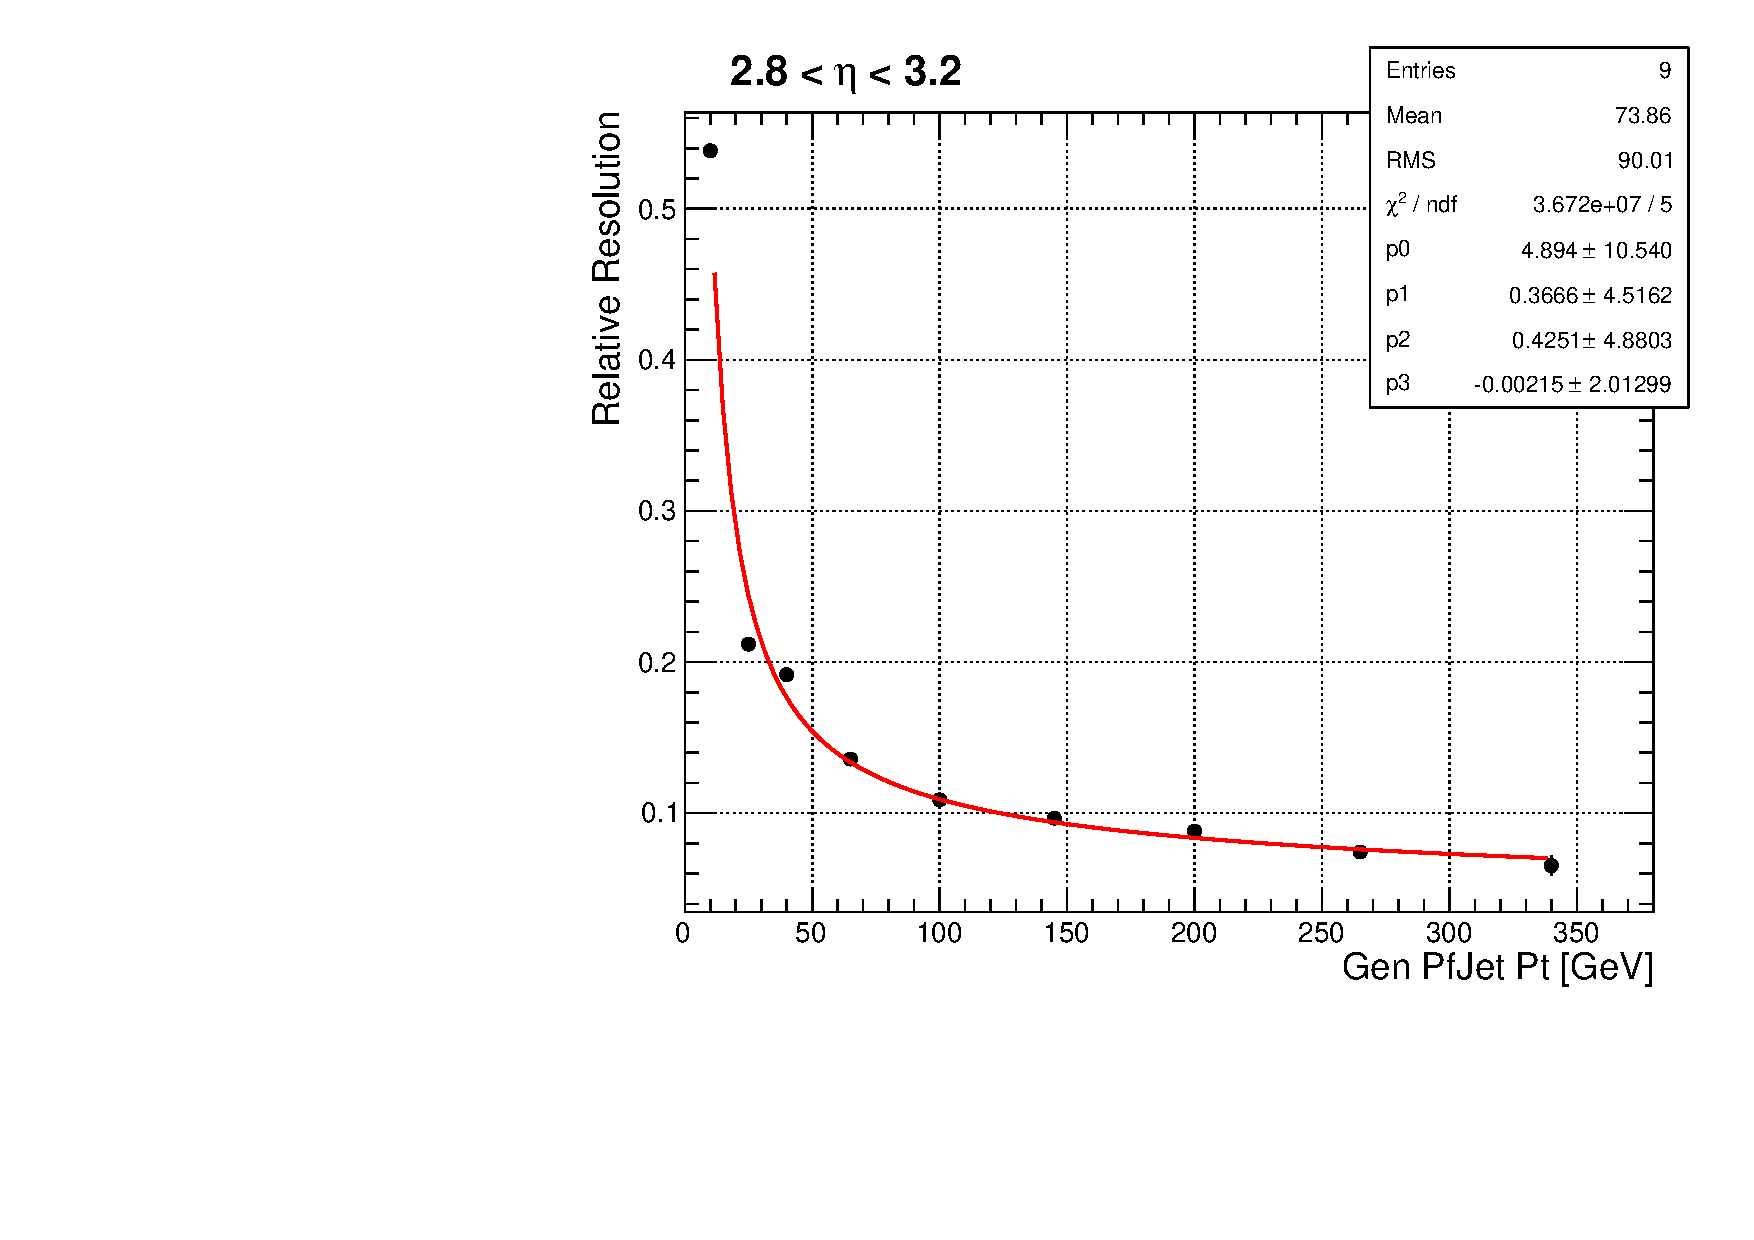
\includegraphics[width=5.3cm,height=5.3cm]{analysis_figs/eta9.pdf}} 
  {\label{fig:fit2e}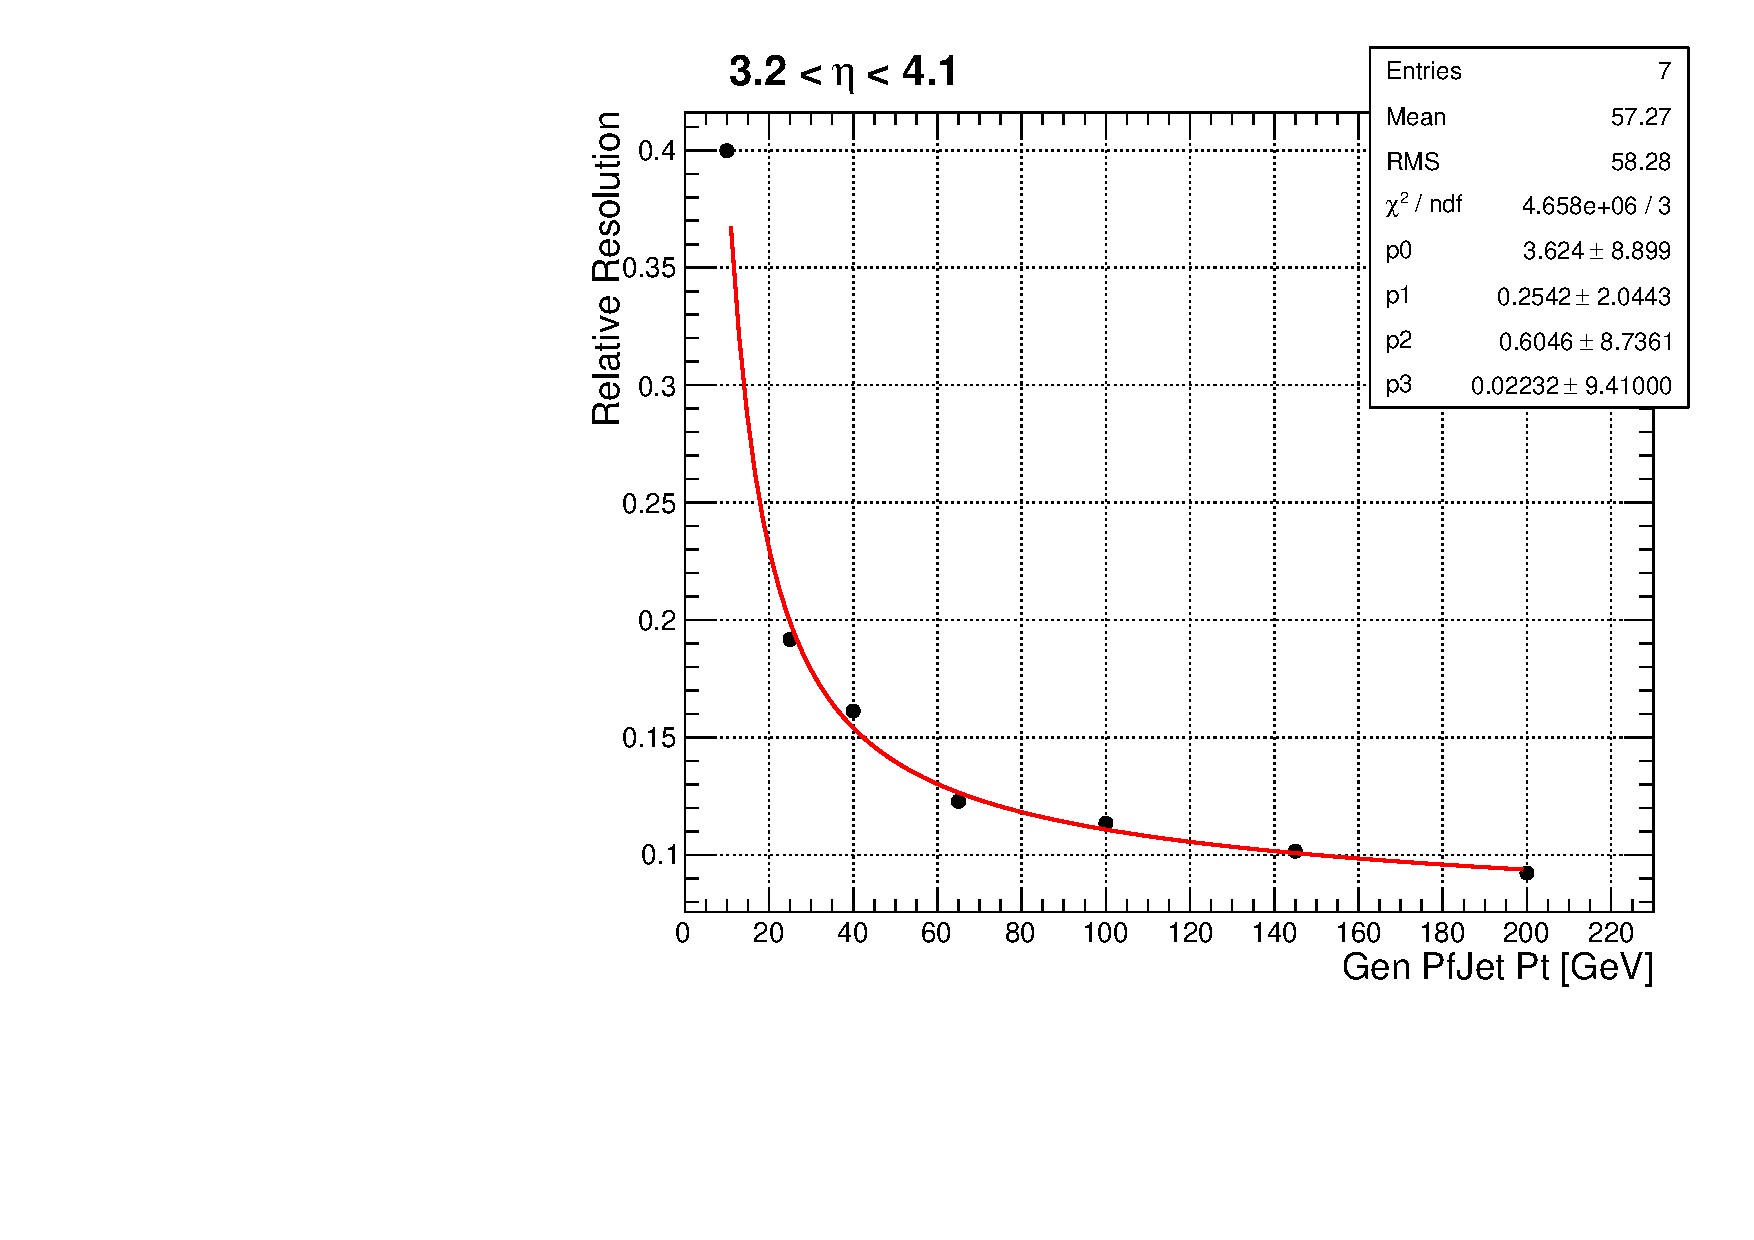
\includegraphics[width=5.3cm,height=5.3cm]{analysis_figs/eta10.pdf}}
  {\label{fig:fit2f}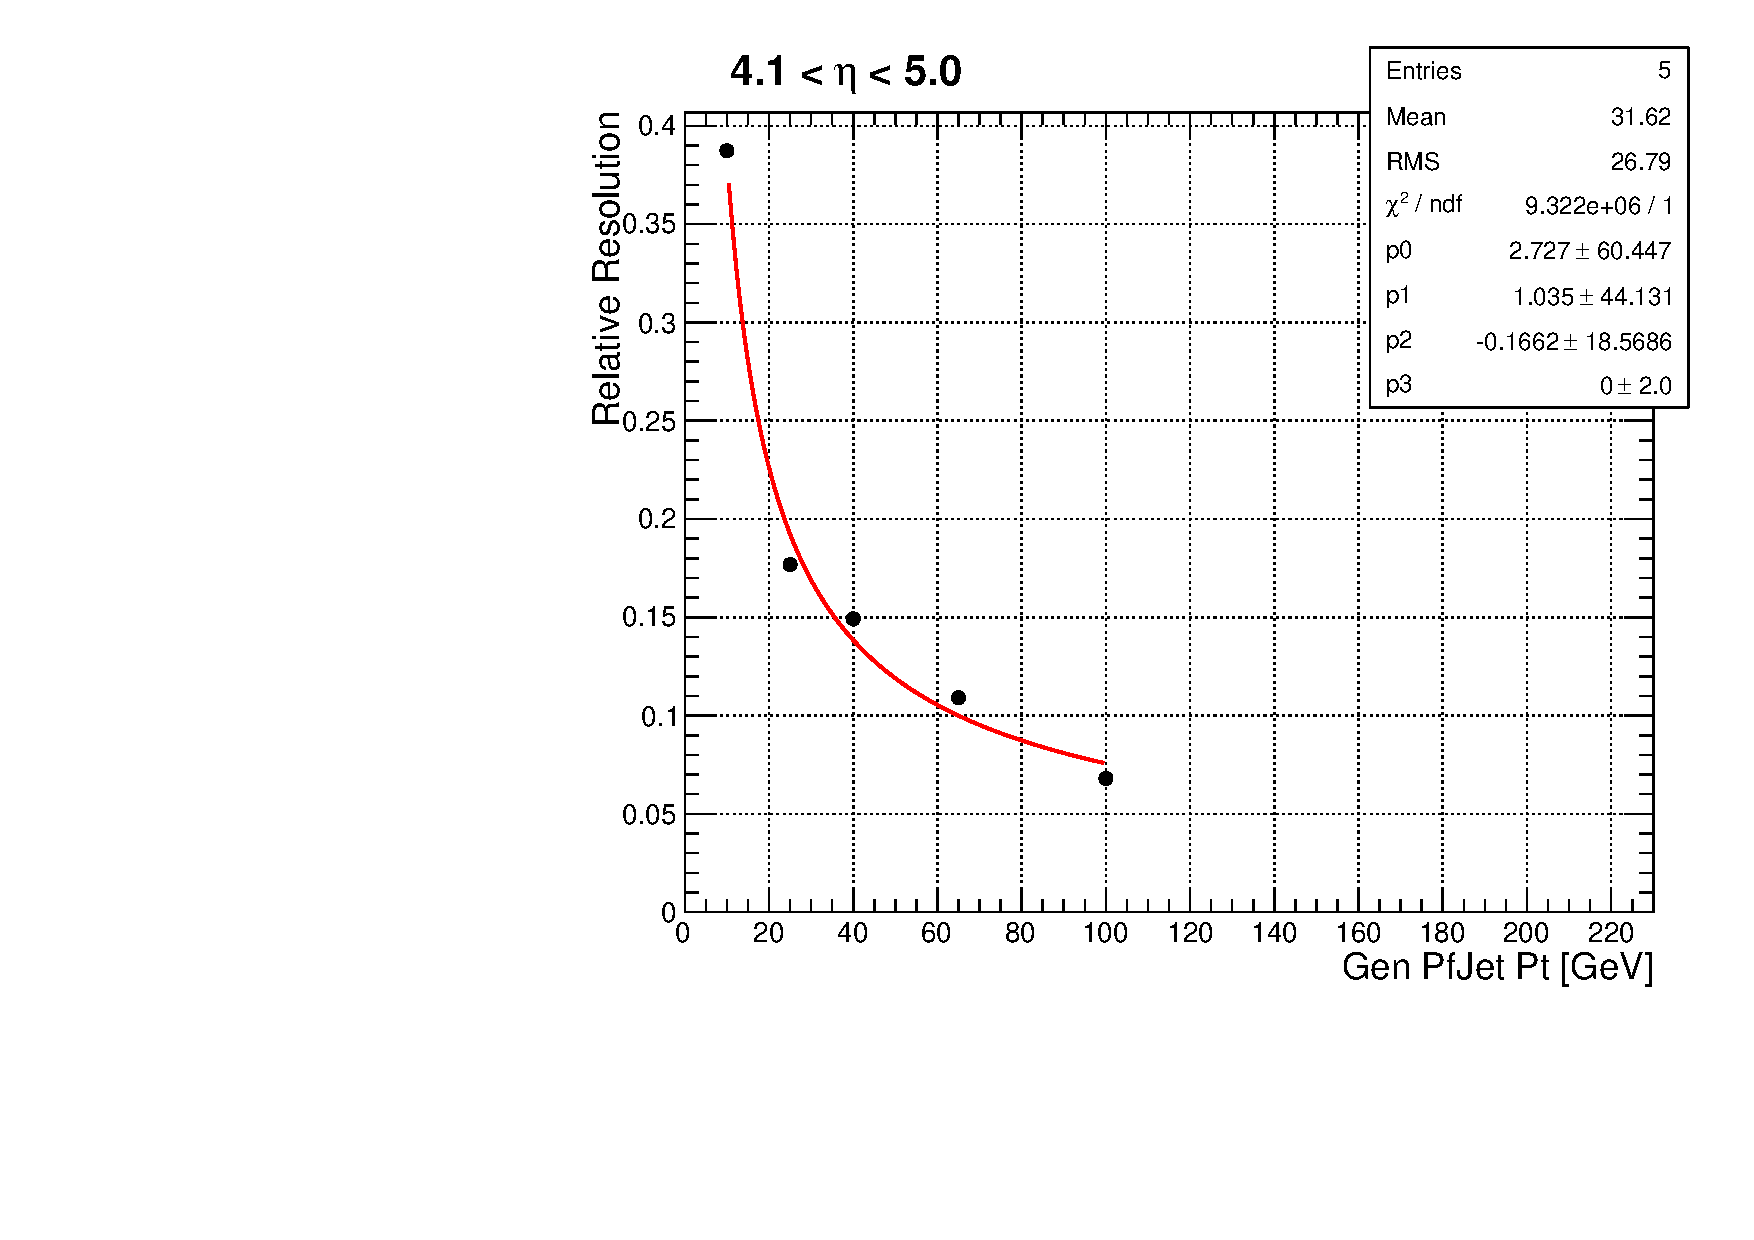
\includegraphics[width=5.3cm,height=5.3cm]{analysis_figs/eta11.pdf}} 
 \caption{ The jet transverse momentum resolution as a function of transverse momentum is given in 12 different $\eta$ ranges continued}
 \label{fig:FIT2}
\end{figure}     

\begin{table}[!h]
\centering
 \caption{Scale Factors for the resolution difference in data and MC}
 \label{jet_table}         
 \begin{tabular}{|c|c|}
   \hline
   Eta Bin     &  Data/MC Ratio ($\pm$ stat. +syst - syst)\\ 
   \hline
   \hline
   0.0 - 0.5       & 1.052 $\pm$ 0.012 + 0.062 - 0.061 \\                        
   0.5 - 1.1     & 1.057 $\pm$ 0.012 + 0.056 - 0.055 \\                        
   1.1 - 1.7    & 1.096 $\pm$ 0.017 + 0.063 - 0.063 \\                        
   1.7 - 2.3     & 1.134 $\pm$ 0.035 + 0.087 - 0.085 \\                        
   2.3 - 5.0     & 1.288 $\pm$ 0.127 + 0.155 - 0.153 \\                        
\hline          
 \end{tabular}
\end{table}

On the other hand, the ${\Em_x}$ and ${\Em_y}$ resolution is calculated as a function of the $\sum E_T - \PT^{gamma}$ in the event to determine the dependence of \met resolution on calorimeter energy resolution. However, as mentioned the major source of uncertainty in the $\met$ measurement is due to jets, i.e. hadronic activity. This is the reason why we can subtract the $\PT^{gamma}$ given that it has excellent resolution.  We have utilized ${\met}$ POG's recent studies to assign the ${\Em_x}$ and ${\Em_y}$ resolution as shown on Fig. \ref{fig:FIT3}. We have also repeated these studies as described in the appendix for our phase space and selection using the controlled data. We have consistent results with the ${\met}$ POG. We have also taken the resolution difference in data and MC into account. The scale factors are provided on Table \ref{met_table}. The functional form used to model the resolutions is \cite{metReso}:

\begin{equation}\label{eq:metreso}
\sigma_{\met} = c_1\sqrt{\sum{\met-q_T}} + c_2 .
\end{equation}

% Add MET RESOLUTION PLOTS and the MET Scale factor table

\begin{figure}[!h]
 \centering
 {\label{fig:fit3a}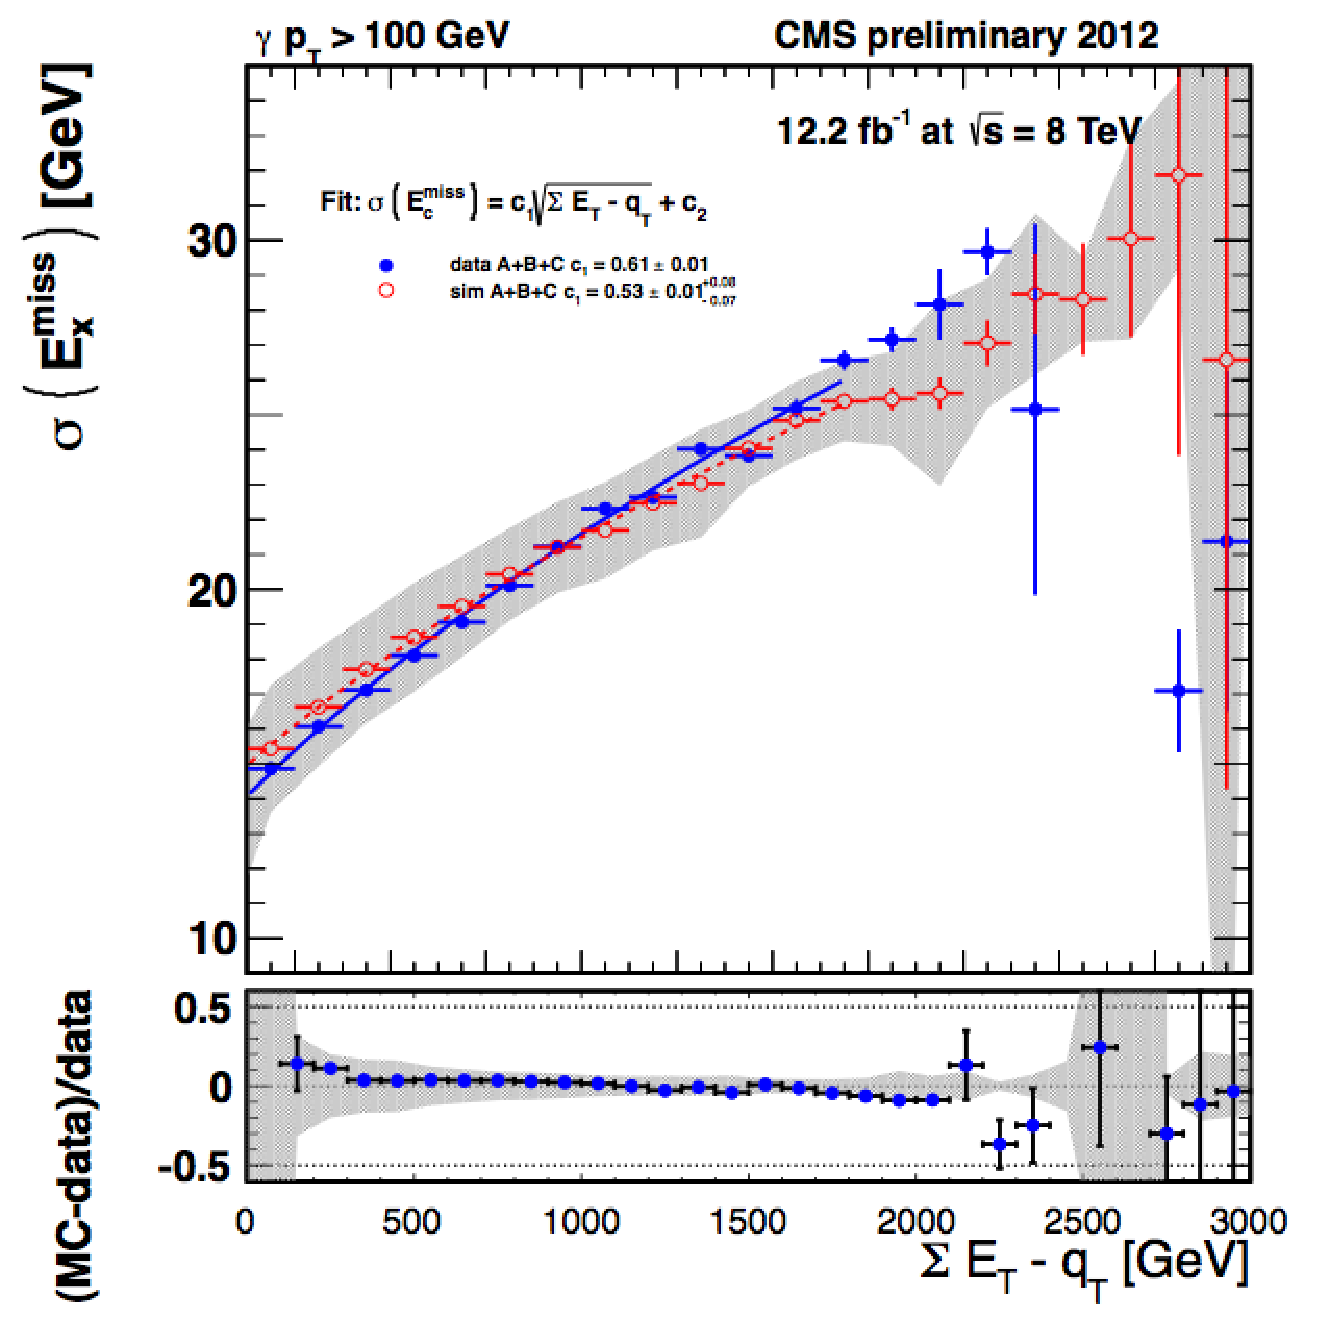
\includegraphics[width=7.5cm,height=7cm]{analysis_figs/ex.pdf}}
 {\label{fig:fit3b}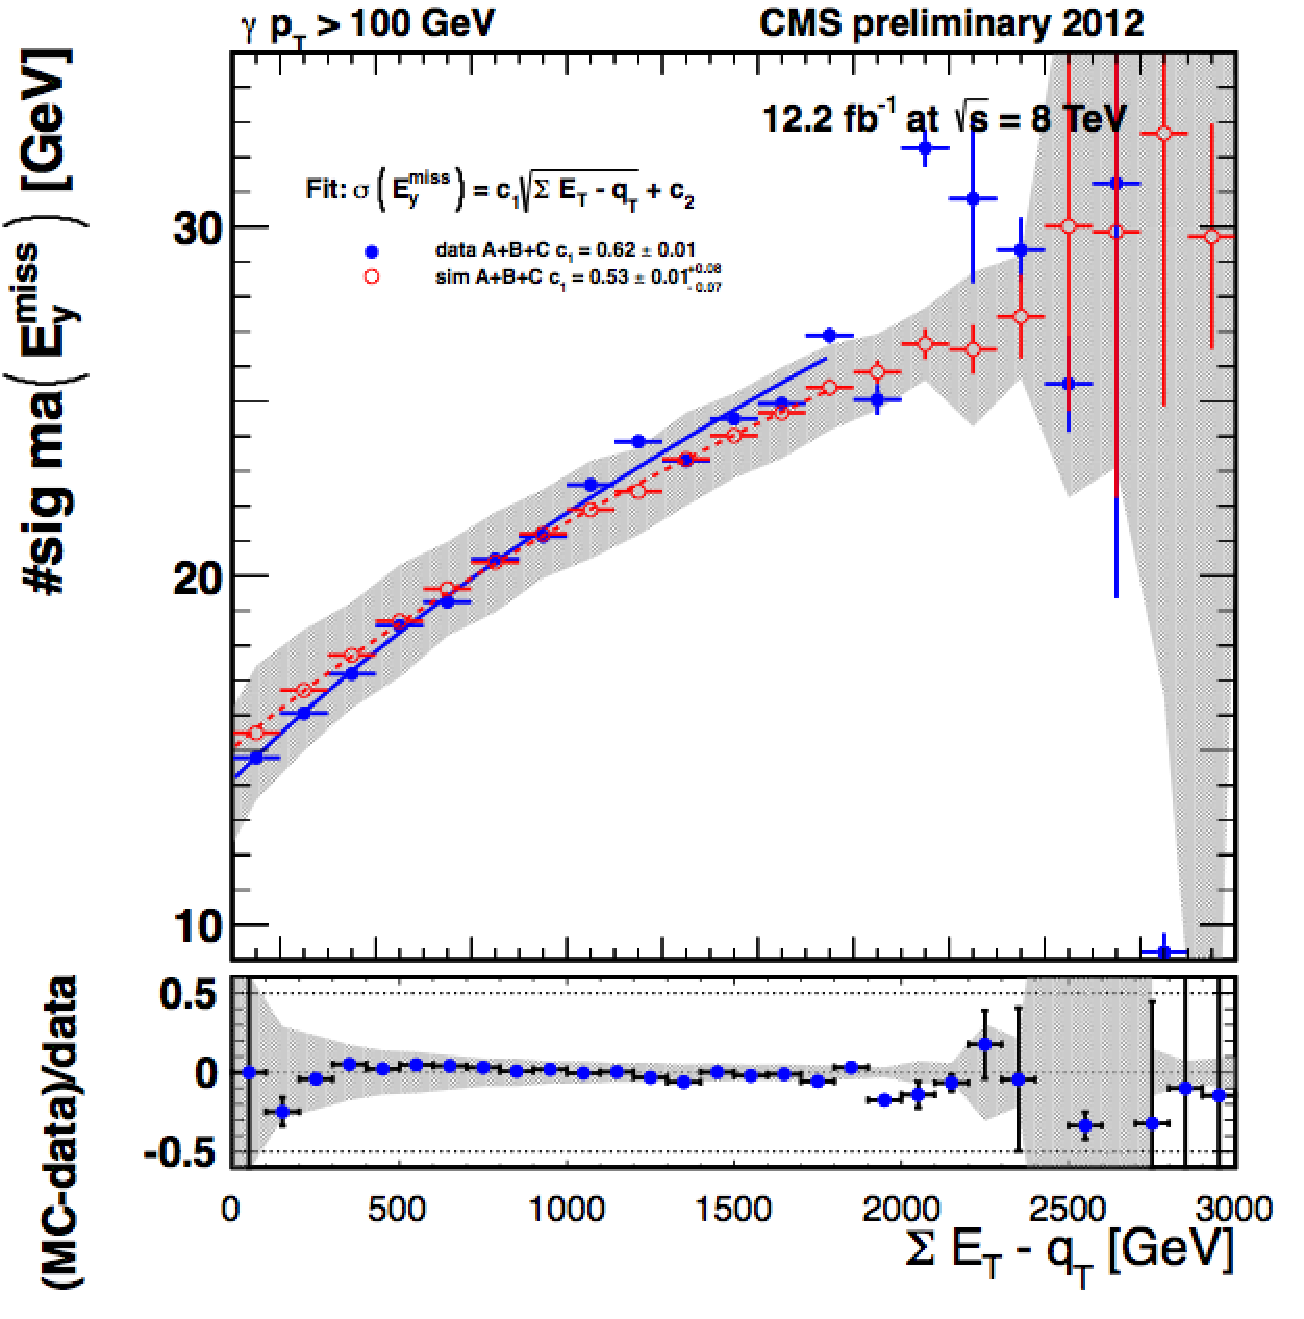
\includegraphics[width=7.5cm,height=7cm]{analysis_figs/ey.pdf}}
  %{\label{fig:fit3a}\includegraphics[width=7.5cm,height=7cm]{analysis_figs/ex_new_rms.pdf}}
  %{\label{fig:fit3b}\includegraphics[width=7.5cm,height=7cm]{analysis_figs/ey_new_rms.pdf}} \\
  %{\label{fig:fit3a}\includegraphics[width=7.5cm,height=7cm]{analysis_figs/ex_new_voig.pdf}}
  %{\label{fig:fit3b}\includegraphics[width=7.5cm,height=7cm]{analysis_figs/ey_new_voig.pdf}}
 \caption{The ${\Em}_{x,y}$ resolution as a function of $\sum{E_T} - \sum{P_T}$ }
 \label{fig:FIT3}
\end{figure}     

\begin{table}[!h]
\centering
 \caption{Scale Factors for the \met resolution difference in data and MC using photon + jet sample}
 \label{met_table}         
 \begin{tabular}{|c|c|c||c|c|}
 \hline
Component     &  $\sigma_{0}$ (GeV) & R = $\sigma_{0}$(data) / $\sigma_{0}$(MC) &  $\sigma_{s}$ ($GeV^{1/2}$) & R = $\sigma_{s}$(data) / $\sigma_{s}$(MC)   \\ 
 \hline
 \hline
   ${\Em_x}$    & 0.37 $\pm$ 0.42 & 0.12 $\pm$ 0.14 $\pm$ 0.19 & 0.61 $\pm$ 0.01 & 1.15 $\pm$ 0.03 $\pm$ 0.15 \\                    
   ${\Em_y}$    & 0.17 $\pm$ 0.37 & 0.05 $\pm$ 0.11 $\pm$ 0.13 & 0.62 $\pm$ 0.01 & 1.17 $\pm$ 0.03 $\pm$ 0.16 \\                    
\hline
 \end{tabular}
\end{table}

Due to having a homogenous ECAL, the energies of photons and electrons are measured very well with very little uncertainty; hence they would not produce a dominant effect in fake  ${\met}$. And due to our lepton veto, the events with muons are rejected.

We have identified the variables that give us a good discrimination between signal and background like events as the probability value of the  $\chi^2$ function (Prob($\chi^2$)) as well as the re-calculated minimized missing ${\met}$.  Both these variables are found to have a good agreement between data and MC. The distributions of these discriminants are shown in Fig. \ref{fig:dist}. It should be noted that the flatness of the Prob($\chi^2$) distribution would serve as an excellent cross check to our understanding and modeling of the resolution. Given that it is mostly flat (with peaks coming from non-gaussian tails of the resolution), it serves as a confirmation that our resolution estimations are good approximations. 

% Add MinMET and P value Plots

\begin{figure}[!h]
 \centering
  {\label{fig:dista}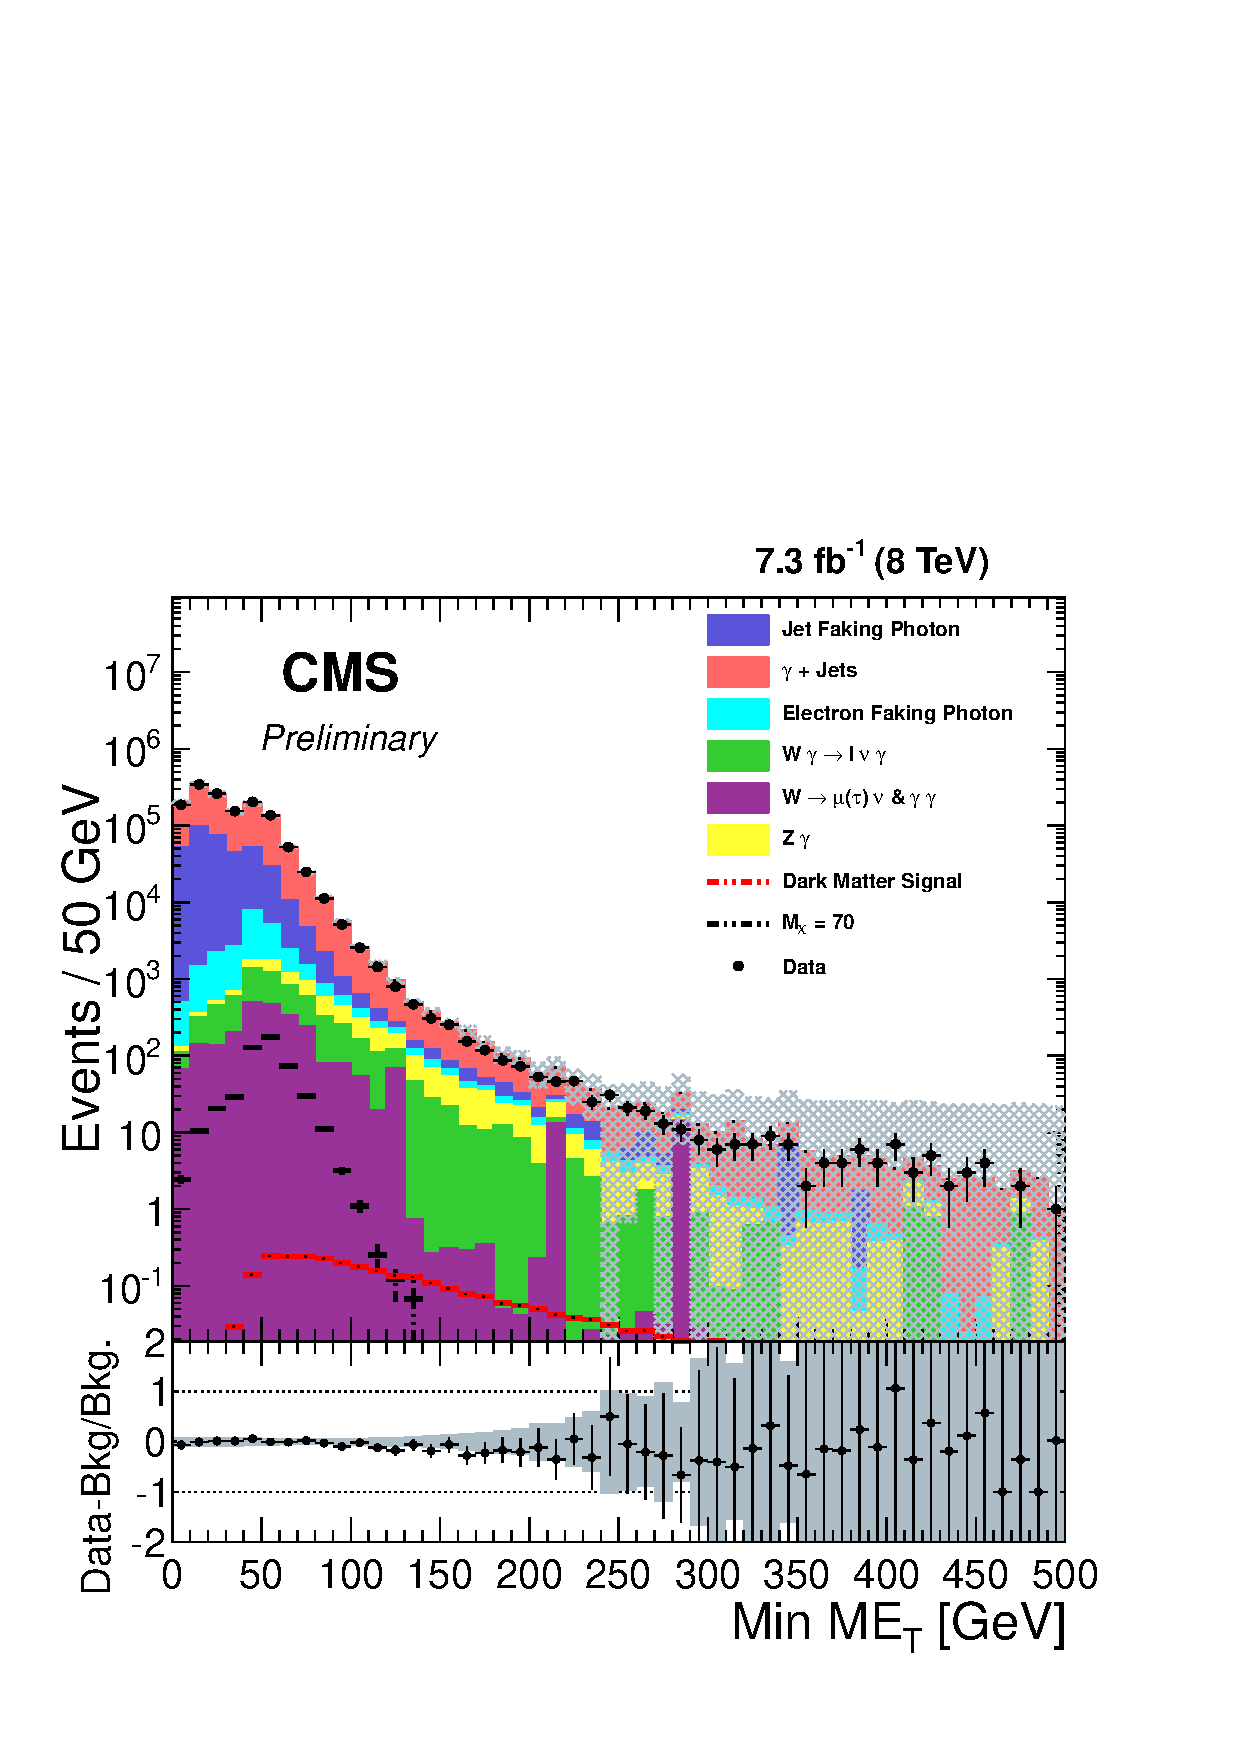
\includegraphics[width=7.5cm,height=7cm]{analysis_figs/StackedHisto_minMET.pdf}}
  {\label{fig:distb}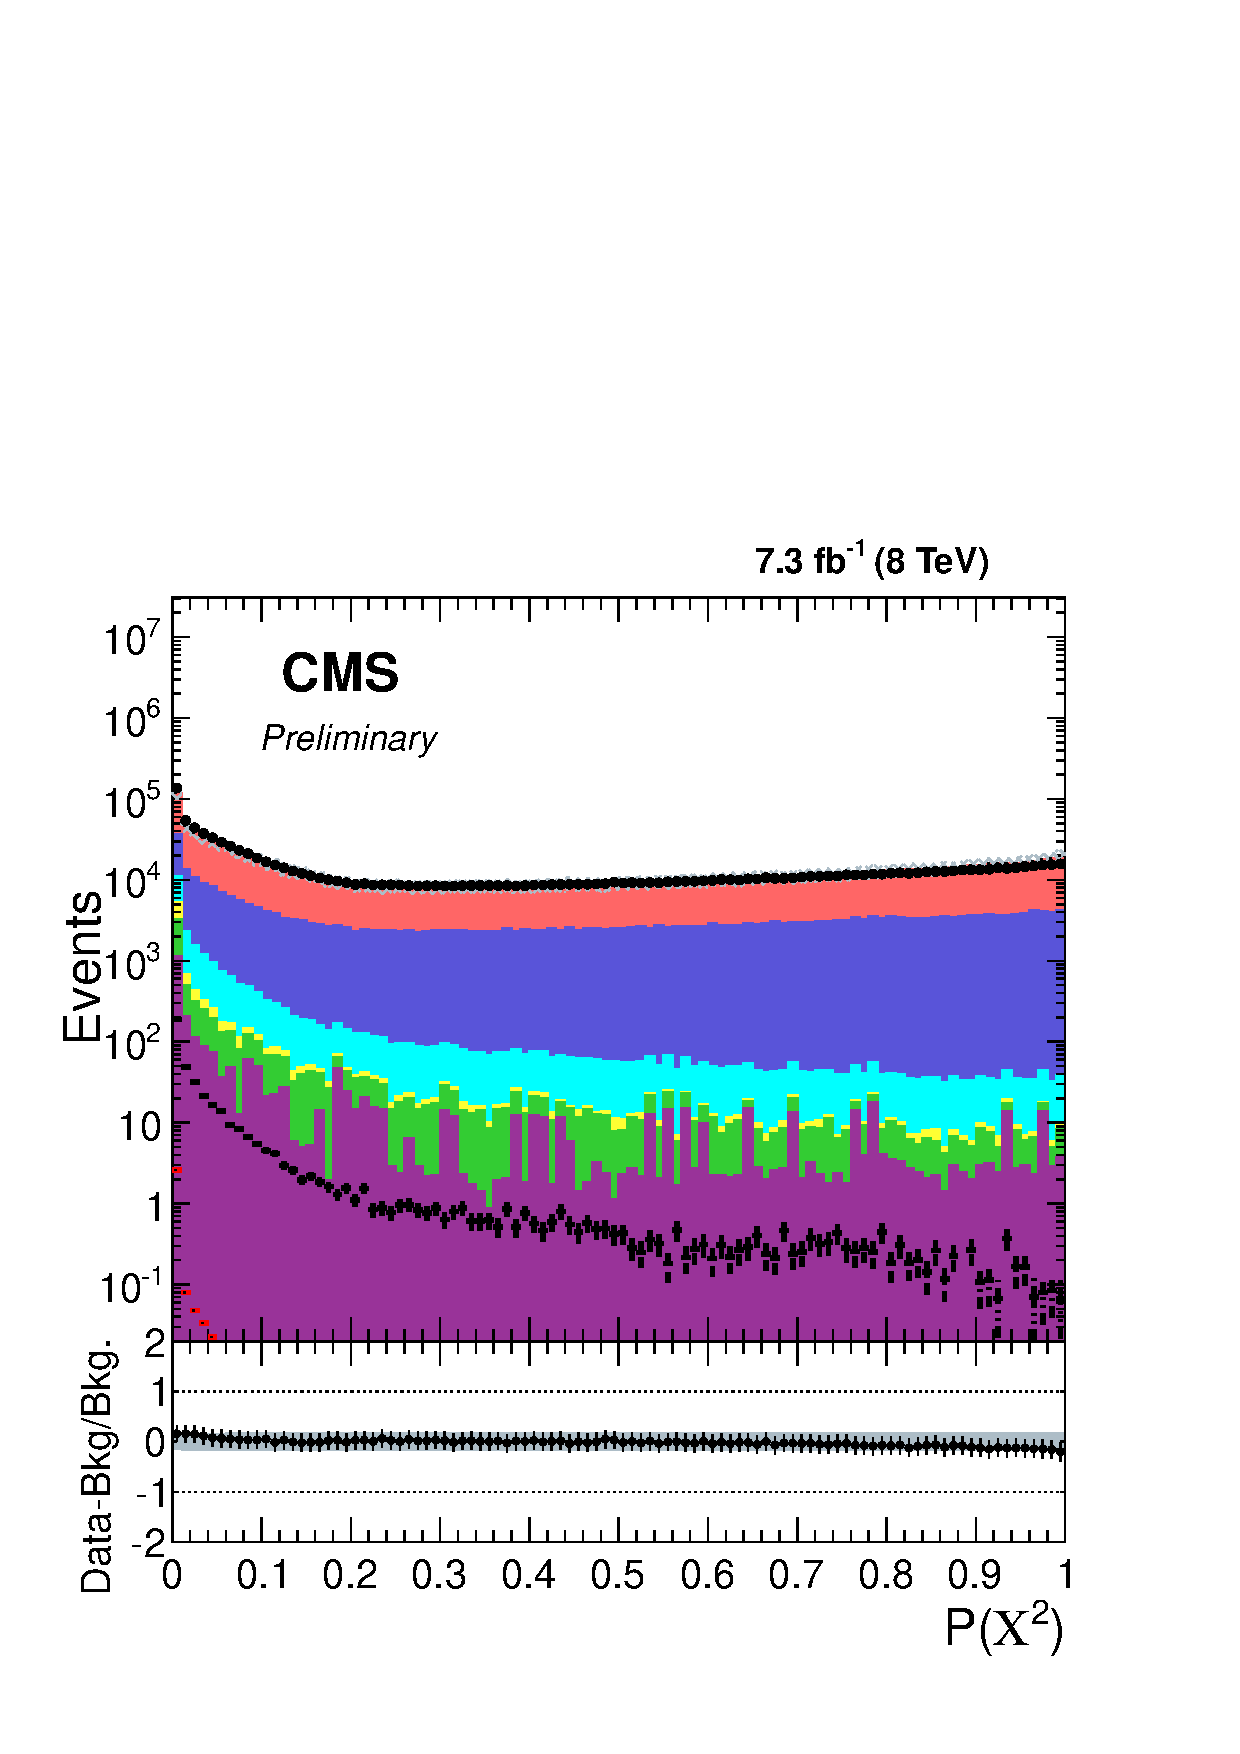
\includegraphics[width=7.5cm,height=7cm]{analysis_figs/StackedHisto_pvalue_notlog.pdf}} 
 \caption{ The probability value of the  $\chi^2$ function and the re-calculated minimized ${\met}$ distributions in data and background predictions. These plots have all the cuts of the analysis, but the proposed MHT cuts. } 
 \label{fig:dist}
\end{figure}   

To emphasize the shape difference in these variables between signal like ($Z\nu\nu\gamma$) and background like ($\gamma + jets$) events, we have looked at the unity normalized distributions. We have also looked at the efficiency of various cut levels with respect to these two processes. The Fig. \ref{fig:perform} shows these distributions. In the minimized MET distribution we see that photon + jet background (where the met is due to mismeasurements) peaks closer to 0, where the $Z\nu\nu\gamma$ background peaks around 45 GeV. This is because we have a cut on the photon \et at 45 GeV, and in the $Z\nu\nu\gamma$ background \met (due to the neutrinos) balances out the energy of the photon. As a result, using this variable one could indentify the events with mismeasured met in the event. Similarly the Prob($\chi^2$) distribution, shows that for event with real \met the minimization resulted in very high values (not successfully minimized the $\chi^2$) where for events with mismeasured \met, the probability distribution is flat.

In conclusion, we require minimized \met $> 45. GeV$ and Prob($\chi^2$) $ < 10^{-3}$.

\begin{figure}[!h]
 \centering
  {\label{fig:distaa}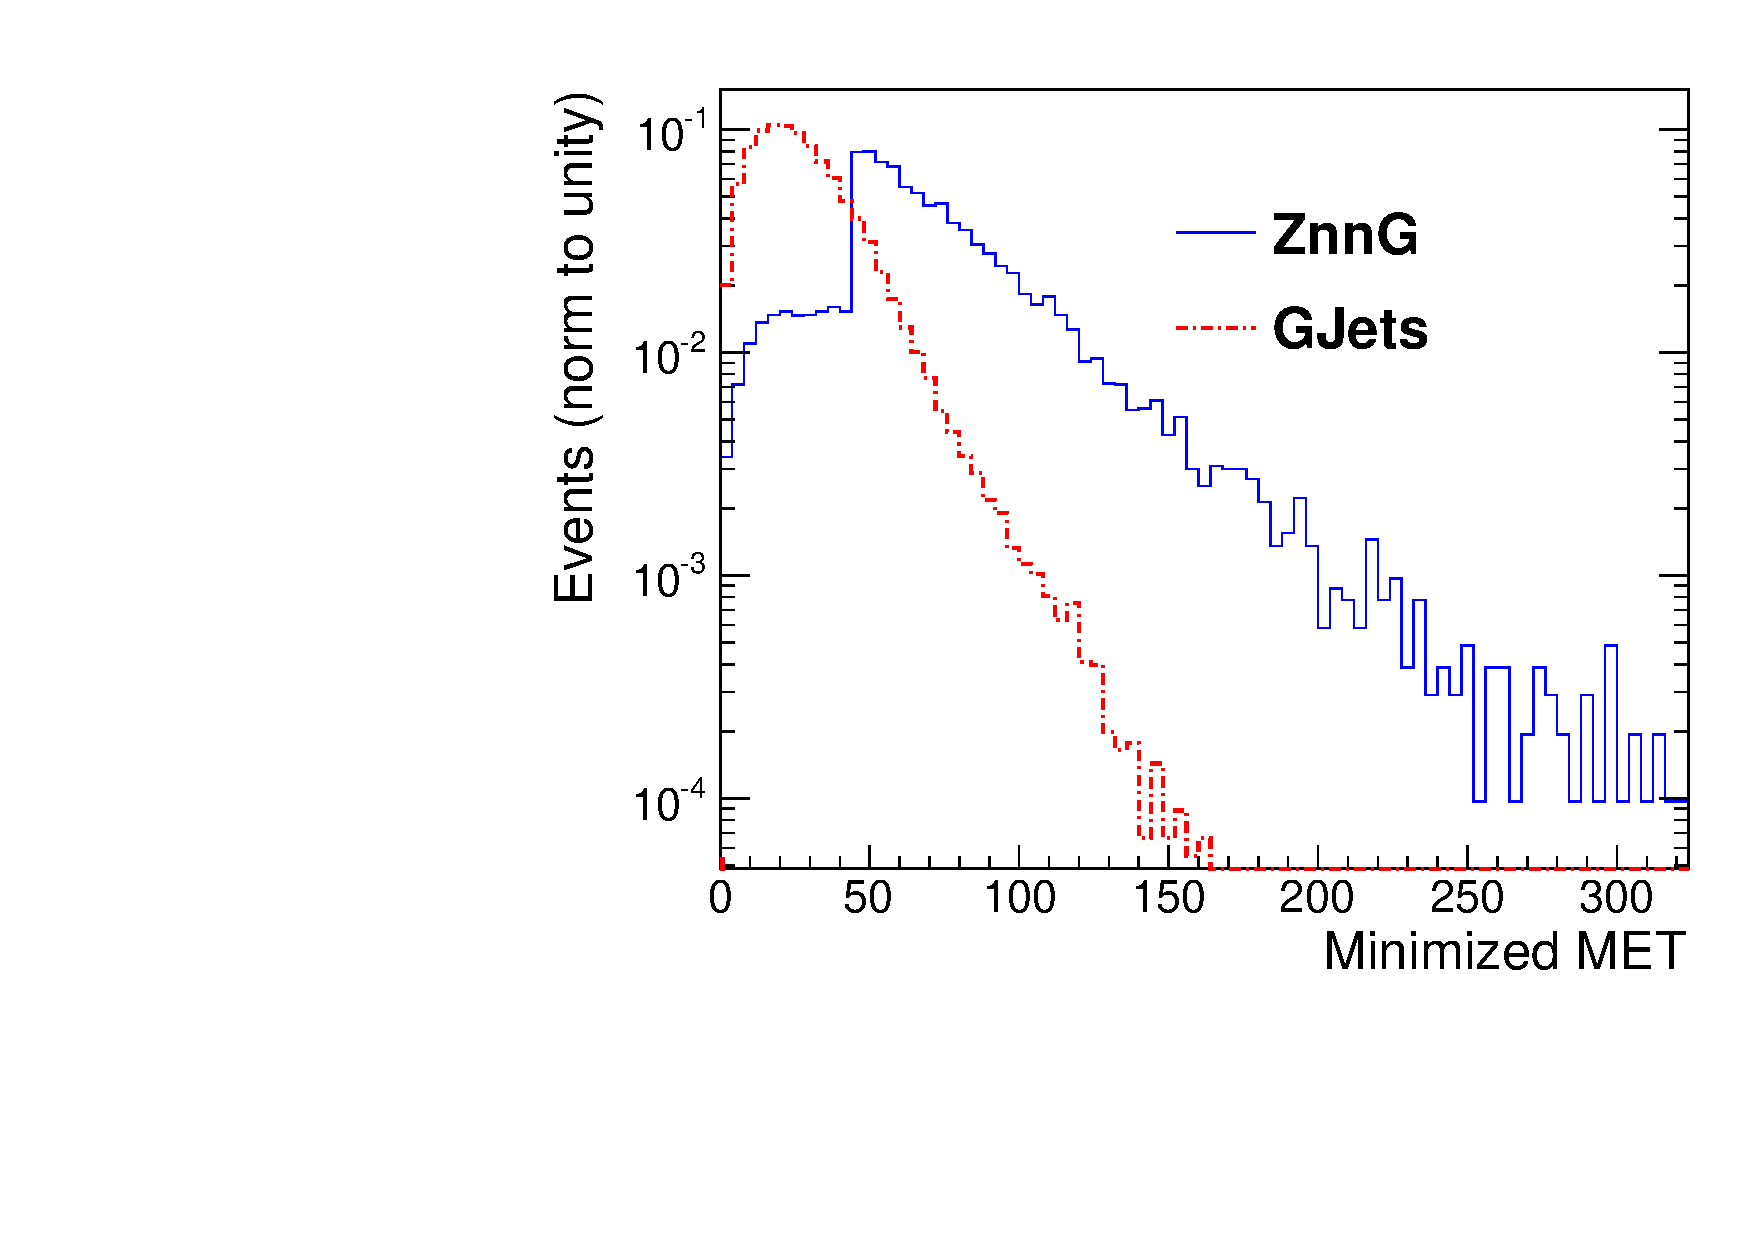
\includegraphics[width=7.5cm,height=7cm]{analysis_figs/minMET.pdf}}
  {\label{fig:distbb}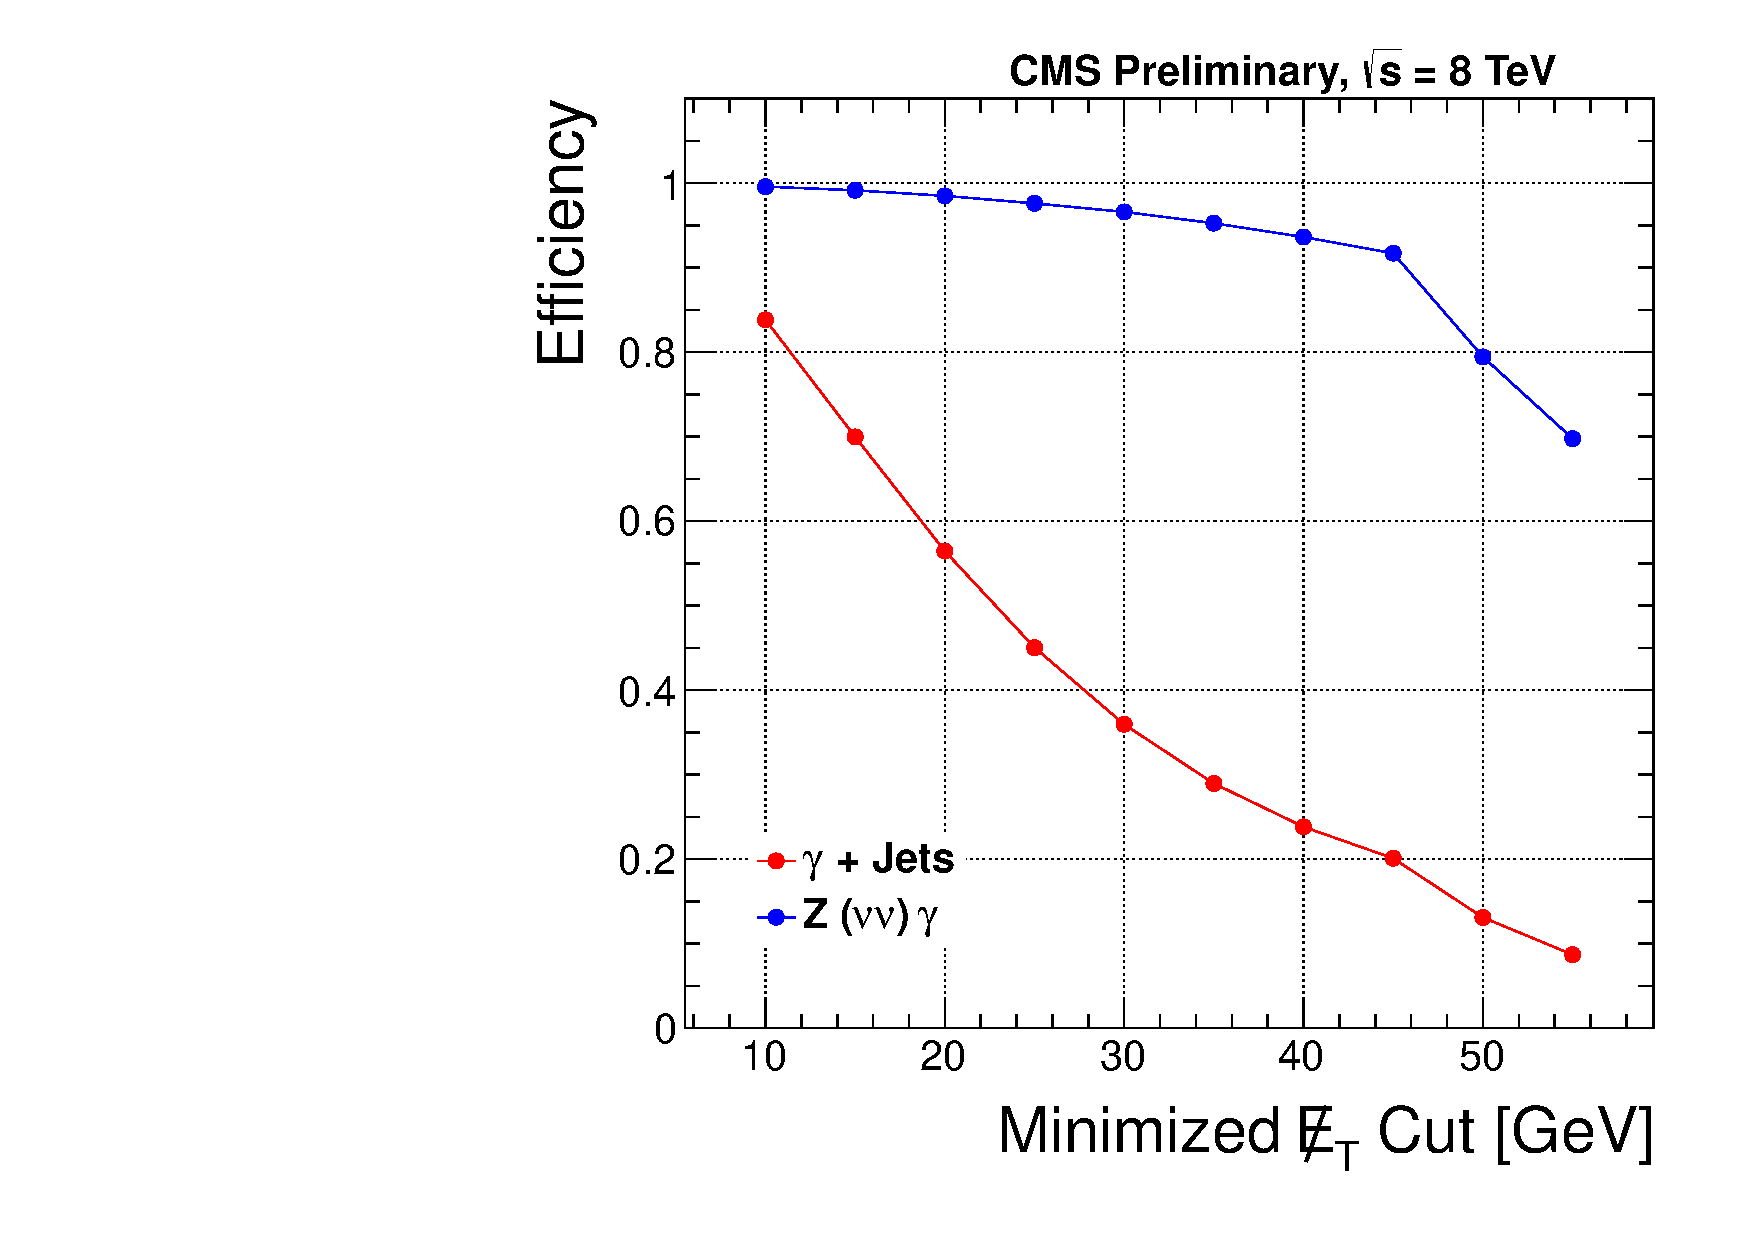
\includegraphics[width=7.5cm,height=7cm]{analysis_figs/roc_minMET.pdf}} \\
  {\label{fig:distcc}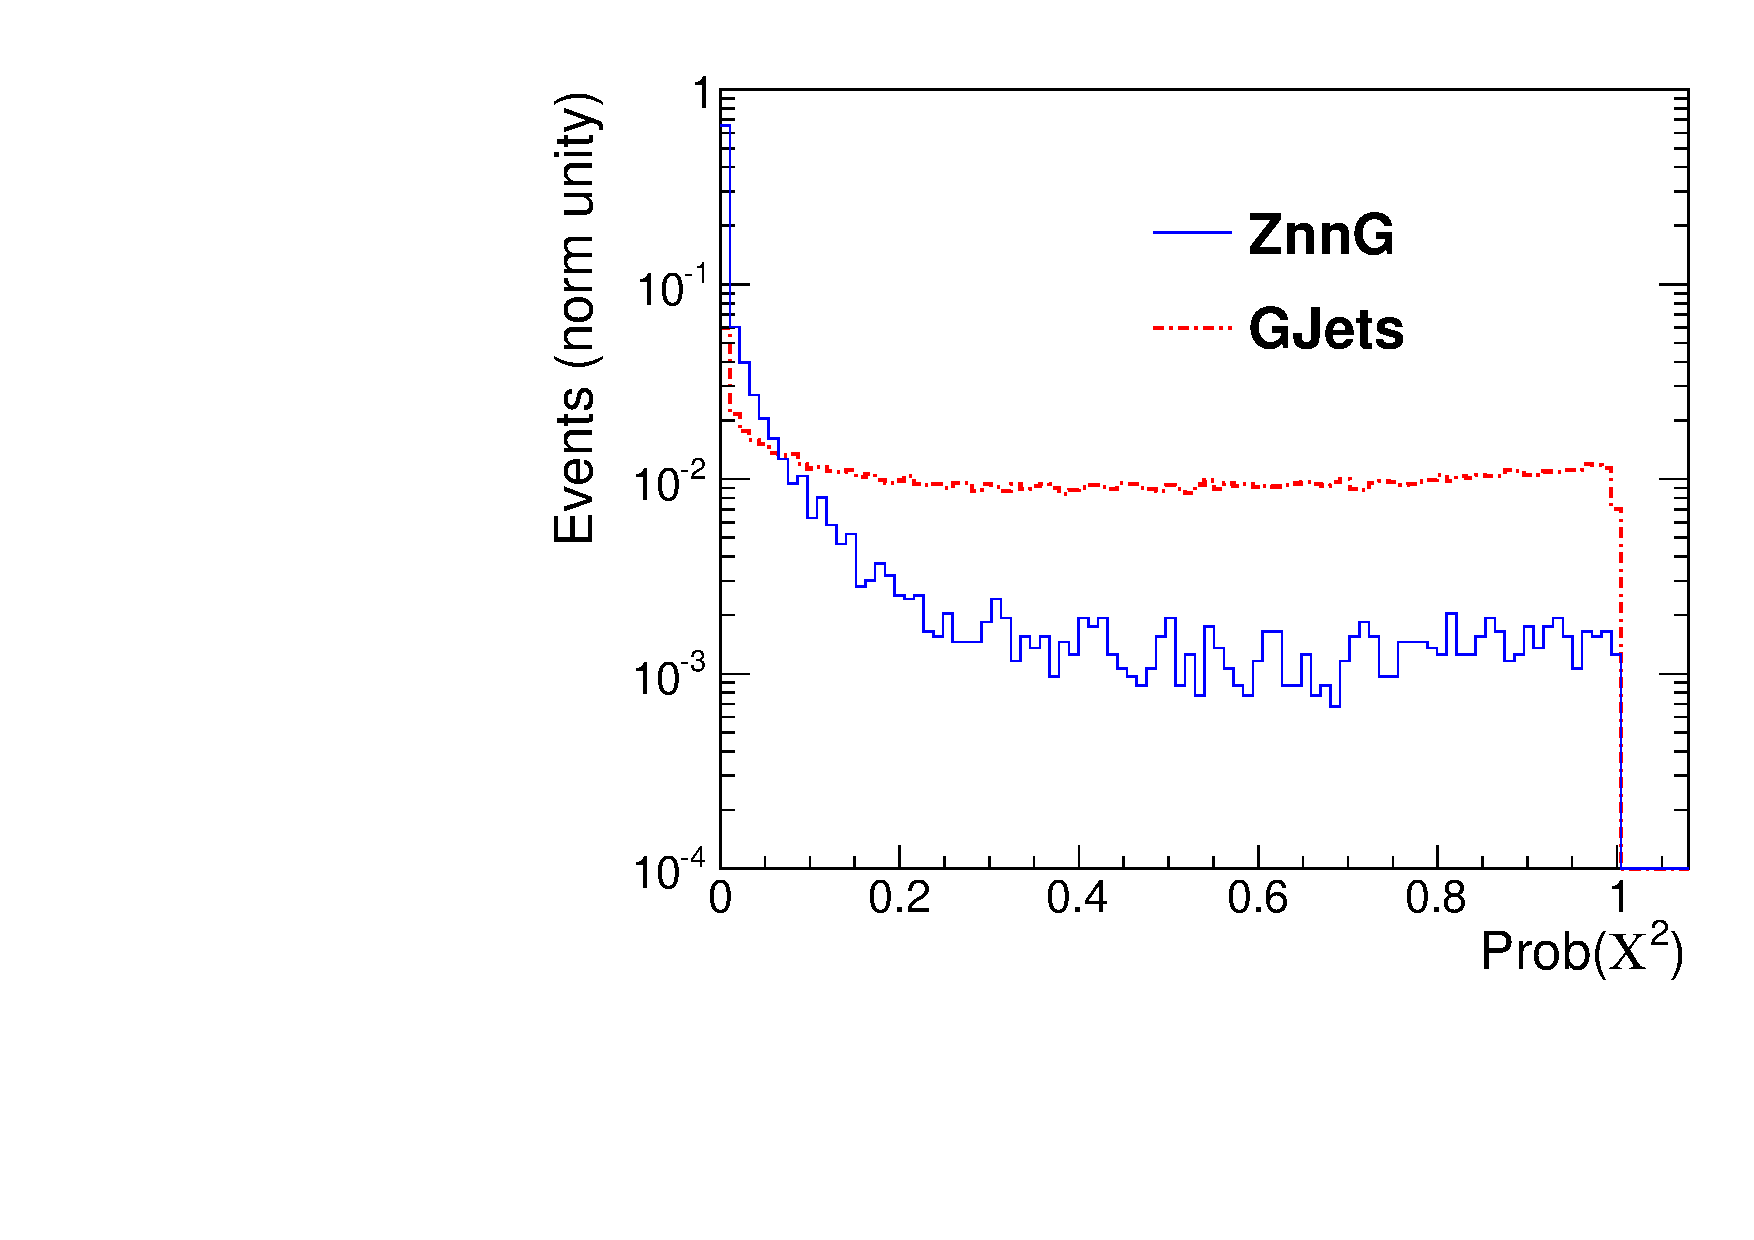
\includegraphics[width=7.5cm,height=7cm]{analysis_figs/pvalue.pdf}} 
  {\label{fig:distdd}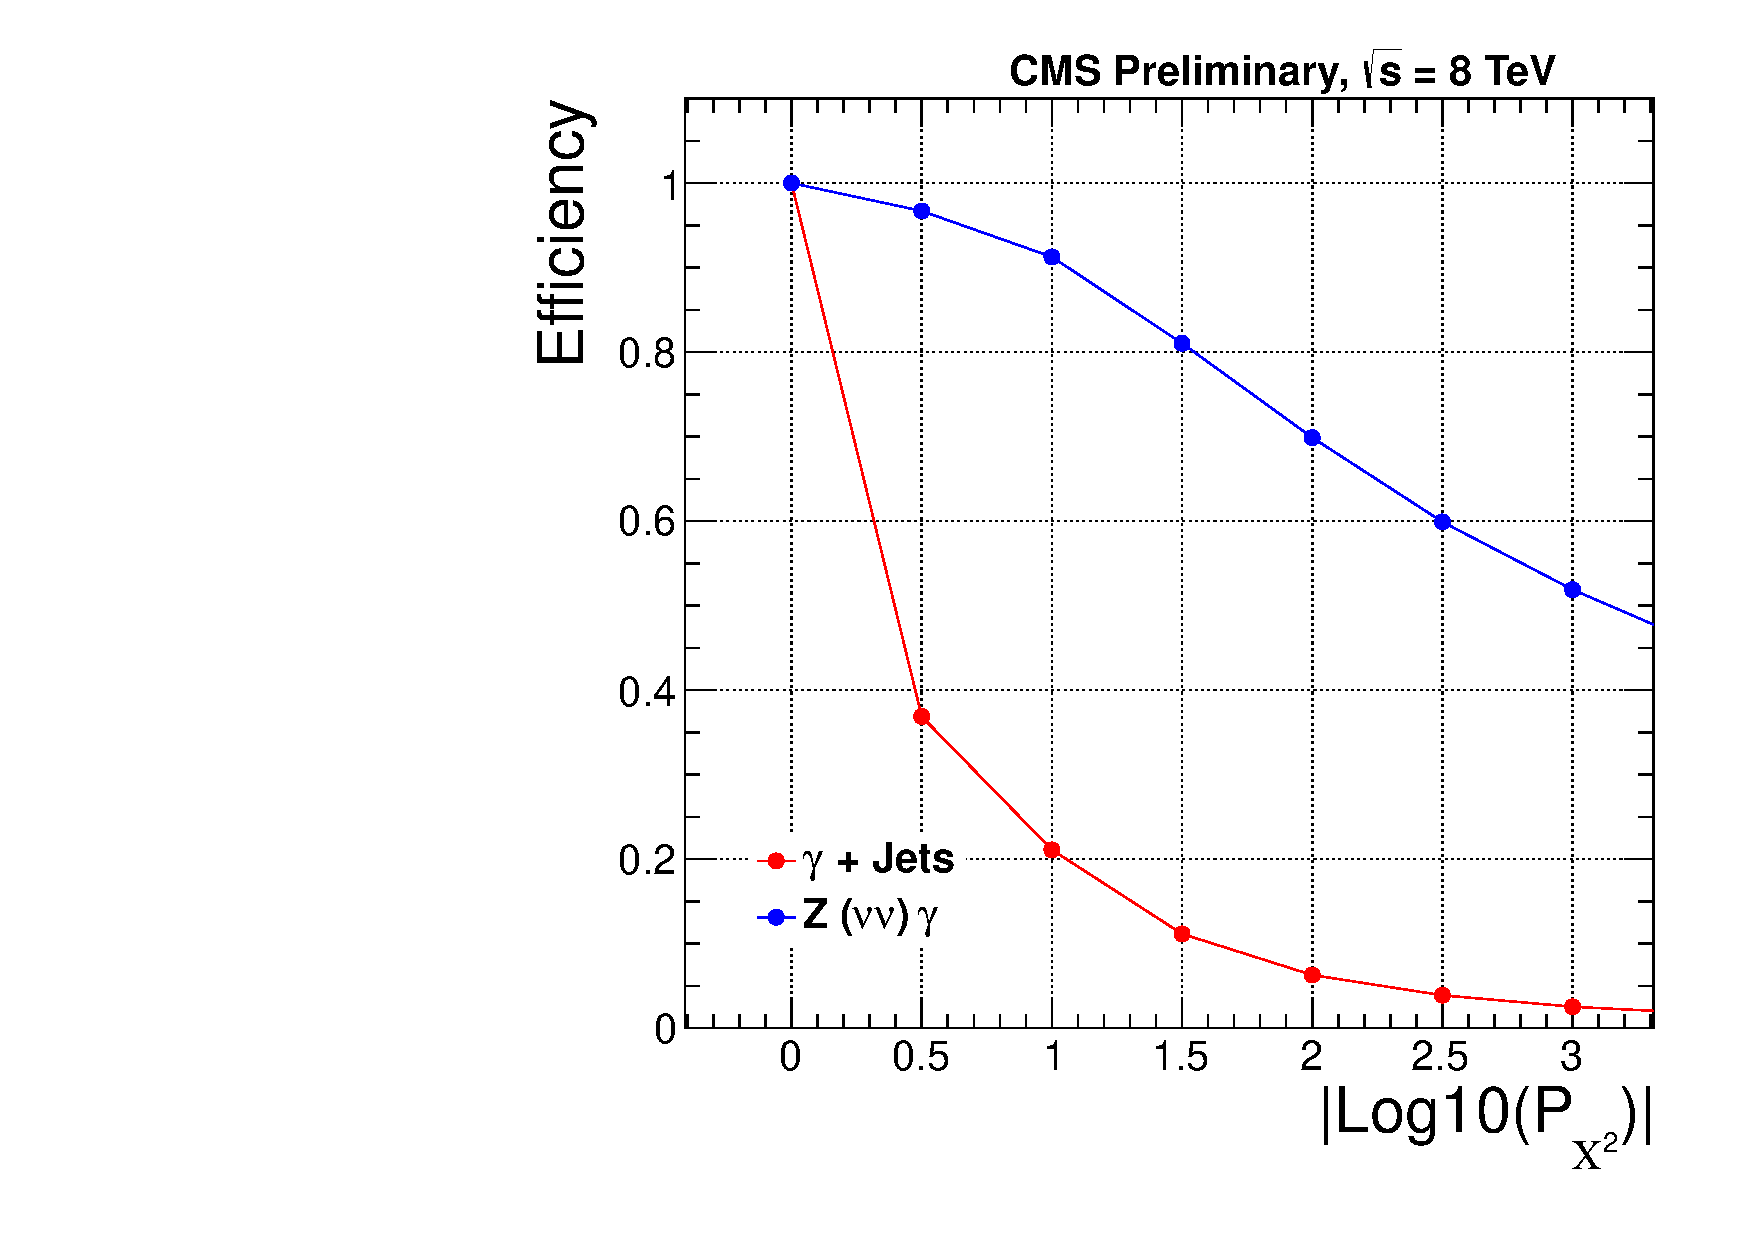
\includegraphics[width=7.5cm,height=7cm]{analysis_figs/roc_pvalue.pdf}}
 \caption{ The shape difference between signal $Z\nu\nu\gamma$ (blue) and background $\gamma + jets$ (red) like processes, along with the ROC Curves. }
 \label{fig:perform}
\end{figure}


% Add some more performance plots

% Add Signal Efficiency plots (as a function of pile up)

%It was further observed that these discriminants had no pile up dependence. This is demonstrated in Fig. \ref{fig:eff}. Using this minimization method, and cutting on the above mentioned value, we reduce our $\gamma +$  jet background by $\sim 80\%$ and QCD background by $\sim 55\%$, while losing only $\sim 1\%$ of the signal. 

%\begin{figure}[!h]
% \centering
%  {\label{fig:effa}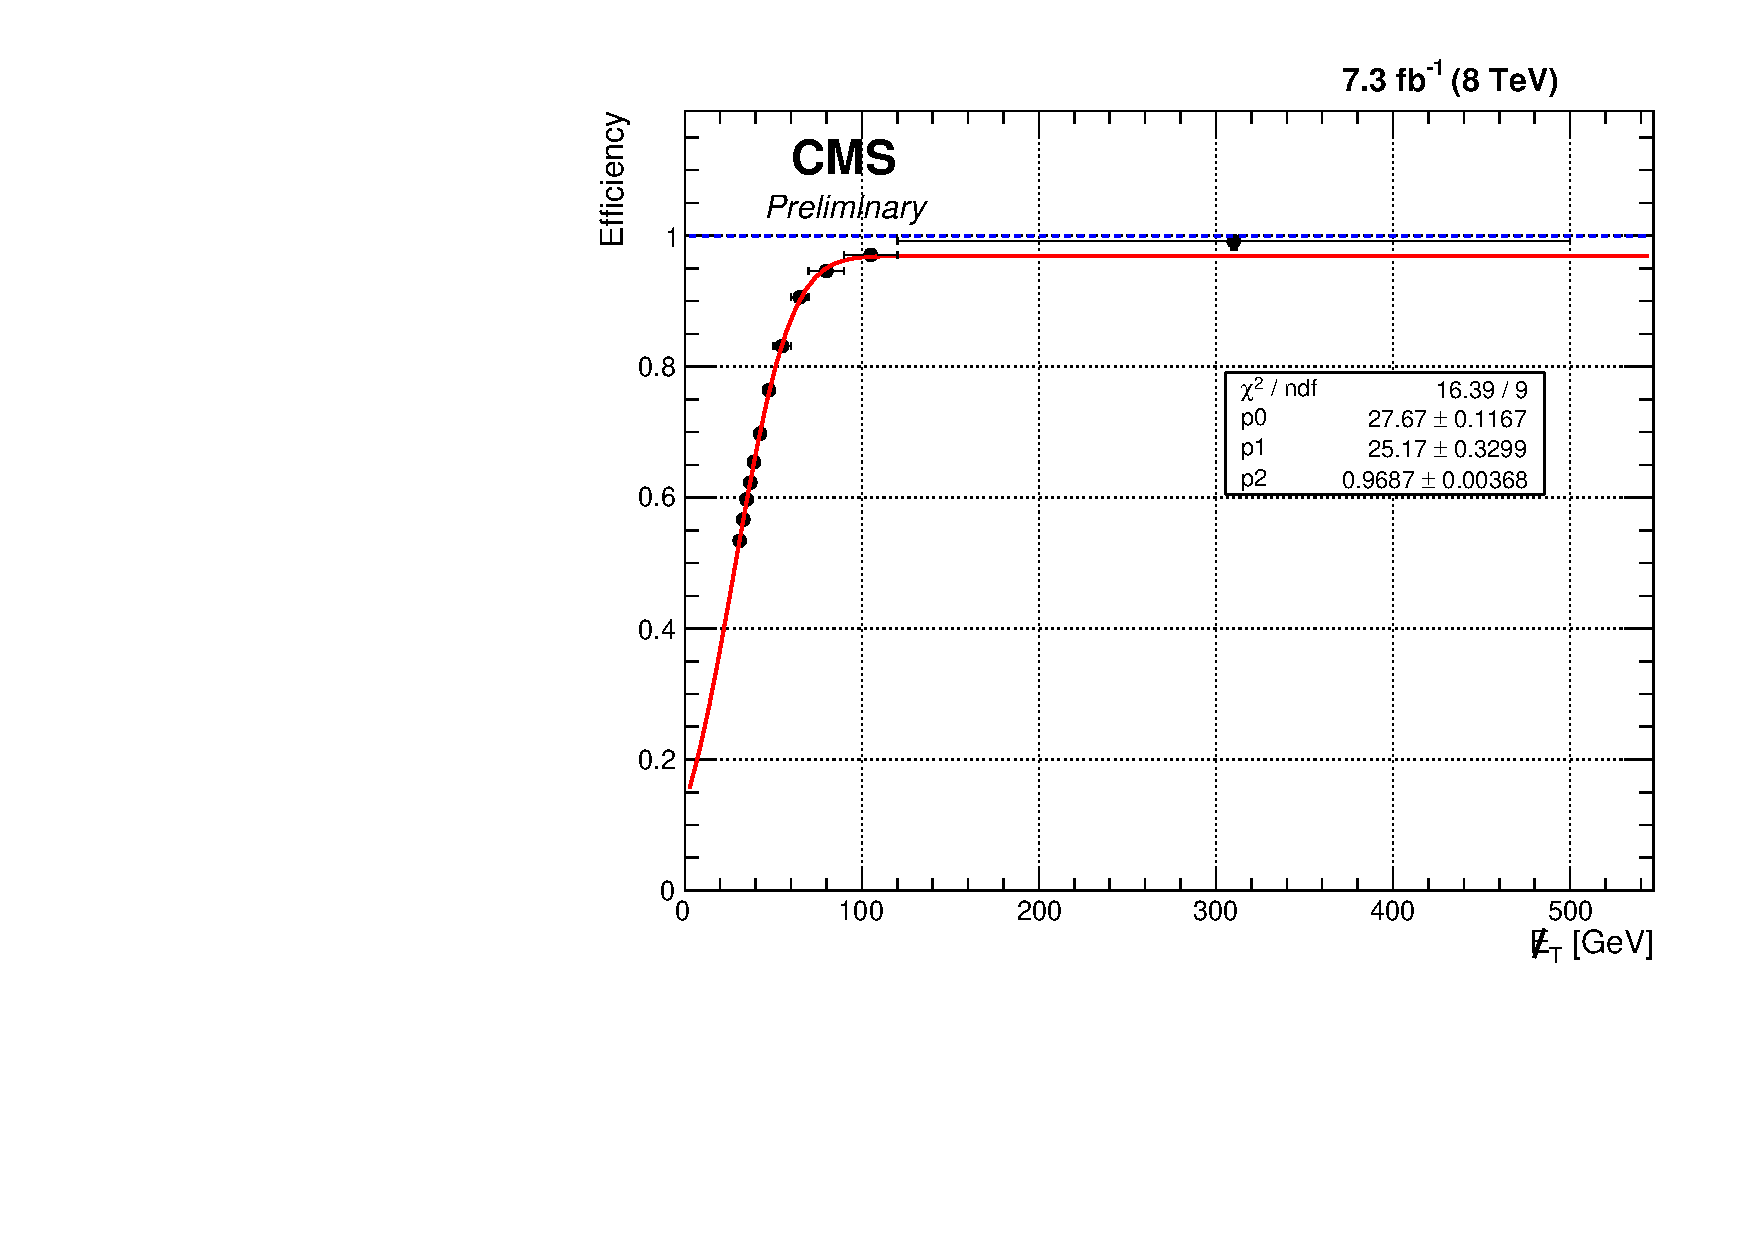
\includegraphics[width=5.3cm,height=5.5cm]{plots/eff_met.pdf}}
%  {\label{fig:effc}\includegraphics[width=5.3cm,height=5.5cm]{plots/bkgeff_mht_Gjet_1400to1800.pdf}}
% \caption{ Efficiency of the new cuts as a function of primary vertices both in signal and background (Photon + Jet for Bins [1400-1800]) predictions. }
% \label{fig:eff}
%\end{figure}   

%The systematic uncertainty introduced by these requirements is assigned using the MET Systematics Tool ~\cite{met}, by shifting jet and photon energy scales up and down, and re-calculating the efficiency. The difference in efficiency is assigned as systematics.
 
%We have also investigated the correlation between the official \met significance method and the method we've developed. Correlation plots for signal ($M_\chi$ = 90 \GeV) and background like events (all $\gamma$ + Jets) can be found in Fig. \ref{fig:correlation}. It was observed that cutting on both values is complementary. Therefore requirements on  both $Prob(\chi^2)$ and \met Significance are applied in this analysis.


%\begin{figure}[!h]
% \centering
%  {\label{fig:corra}\includegraphics[width=5.3cm,height=5.5cm]{analysis_figs/bkg_corr.pdf}}
%  {\label{fig:corrb}\includegraphics[width=5.3cm,height=5.5cm]{analysis_figs/sig_corr.pdf}}
% \caption{ 2D correlation plots for \met Significance and MHT Minimization}
% \label{fig:correlation}
%\end{figure}   

